\documentclass[12pt,a4paper]{book}

\usepackage[table,dvipsnames,svgnames]{xcolor}
\usepackage{listingsutf8}
%\usepackage[utf8]{inputenc}% gestion des accents (source)
\usepackage[T1]{fontenc}% gestion des accents (PDF)
\usepackage{fontspec}
\usepackage[french]{babel}% gestion du français
\usepackage{textcomp}% caractères additionnels
\usepackage{mathtools,amssymb,amsthm}% packages de l'AMS + mathtools
\usepackage{amsmath}
\usepackage{yhmath}
\usepackage{mathpazo}
\usepackage[scaled=0.95]{helvet}
\usepackage{courier}
%\usepackage{fourier}
%\usepackage[scaled=0.95]{helvet}
%\usepackage{courier}
\usepackage{bm}
\usepackage{gensymb}
\usepackage{graphicx}

\usepackage{enumitem}
\usepackage{pifont}

\usepackage{pstricks}
\usepackage{pstricks-add}
\usepackage{pst-eucl}
\usepackage{pgfplots}
\let\clipbox\relax
%\usepackage{pst-plot,pst-text,pst-tree,pstricks-add}
%\usepackage{pst-node} % required package
\usepackage{pst-all}
\usepackage[most,skins,breakable]{tcolorbox}

\usepackage{euscript}





% ############### Nouvelles commandes ###############
% Coloration des labels des points dans pst-eucl
\makeatletter
\define@key[psset]{pst-eucl}{LabelColor}{\def\psk@LabelColor{#1}}
\psset{LabelColor=black}
\def\Pst@WhichLabel#1{{\color{\psk@LabelColor}%
		\ifx\psk@PointName\@default#1\else\psk@PointName\fi}}
\makeatother

% renomme le symbole #2 en #1#2 et invalide le symbole initial #2:
\def\renamesymbol#1#2{
	\expandafter\let\expandafter\newsym\expandafter=\csname#2\endcsname
	\expandafter\global\expandafter\let\csname#1#2\endcsname=\newsym
	\expandafter\global\expandafter\let\csname#2\endcsname=\origsym
}



\usepackage{ProfCollege}
\renamesymbol{Casio}{Calculatrice}
\usepackage[nonshellescape]{ProfLycee}



%\usepackage[left=1.5cm,right=1.5cm,top=2.5cm,bottom=2.5cm]{geometry}
\usepackage[left=13mm,right=13mm,top=18mm,bottom=18mm,footskip=30pt]{geometry}
\setlength{\headheight}{15pt}

\usepackage{titlesec}
\usepackage{pas-math}
\usepackage{longtable}
\usepackage{tikz,tkz-tab}
\usepackage{amsmath}
\usepackage[right]{eurosym}
\usepackage{sectsty}
\usepackage{tipfr}
\usepackage{setspace}

%pour faire les touches de la calculatrices
\usepackage{menukeys}
\renewmenumacro{\menu}{roundedmenus} % default: menus
\renewmenumacro{\directory}{pathswithfolder} % default: paths
\renewmenumacro{\keys}{shadowedroundedkeys} % default: roundedkeys


\usepackage{multicol}
\usepackage{multirow}
\usepackage{systeme}

%% Format des titres de chapitres, paragraphes, ...
\titleformat{\chapter}[frame]
{\color{red!85!white}\normalsize}%
{\filright\sffamily\Large%
	\enspace Chapitre \thechapter\enspace}%
{8pt}
{\color{red!85!white}\rule{0pt}{30pt}\sffamily\Huge\bfseries\filcenter}
%%%%%%%%%%%%%%%%%%%%
\titlespacing{\chapter}{0pc}{0pc}{2pc}
\titlespacing{\subsection}{2pc}{}{}

\titleformat{\subsection}[block]{\hspace{1em}}{\thesubsection}{1em .}{}
\titleformat{\subsubsection}[block]{\hspace{2em}}{\thesubsection}{1em )}{}

\chapterfont{\color{red}{}}
\sectionfont{\color{green!55!black}{}}
\subsectionfont{\color{cyan!65!black}{}}
\subsubsectionfont{\color{violet}{}}
\renewcommand{\thesection}{\color{green!55!black}\Roman{section}.}
\renewcommand{\thesubsection}{\color{cyan!65!black}\arabic{subsection})}
\renewcommand{\thesubsubsection}{\color{violet}\alph{subsubsection})}
\setcounter{secnumdepth}{3}

\titleformat{\subsection}[block]{\hspace{1em}}{\thesubsection}{1em .}{}
\titleformat{\subsubsection}[block]{\hspace{2em}}{\thesubsection}{1em )}{}

\usepackage[column=A]{cellspace}
\setlength{\cellspacebottomlimit}{4pt}
\setlength{\cellspacetoplimit}{4pt}
\setlength{\parindent}{2pt}
\setlength{\tabcolsep}{0.5cm}


%entête et pieds de pages
\usepackage{fancyhdr}
\pagestyle{fancy}
\fancyhf{}
\usepackage{lastpage}
\renewcommand{\chaptermark}[1]{\markboth {Chap. \thechapter~ - ~#1}{}}
\renewcommand\headrulewidth{1pt}
\fancyhead[LO,RE]{1ère G - spécialité maths}
\fancyhead[RO,LE]{\leftmark}
\renewcommand\footrulewidth{1pt}
\fancyfoot[LO,RE]{Année 2025-2026}
\fancyfoot[RO,LE]{\textbf{Page \thepage/\pageref{LastPage}}}

%Mes boites pour les définitions, propriétés, remarques, ...

%Mes boites pour les définitions, propriétés, remarques, ...

\newcommand\titrebox[1]{\textbf{#1}}
\newtcolorbox{definition}{breakable,colback=red!10!white,
	colframe=red!85!white, fonttitle=\bfseries,enhanced,
	attach boxed title to top left={xshift=5mm, yshift=-2mm},boxed title style={size=small,colback=red!10!white,colframe=red!85!white, arc=0.5mm},
	title=\textcolor{red!85!white}{Définition} , arc=3mm}

\newtcolorbox{definitionTitre}[1]{breakable,colback=red!10!white,
	colframe=red!85!white, fonttitle=\bfseries,enhanced,
	attach boxed title to top left={xshift=5mm, yshift=-2mm},boxed title style={size=small,colback=red!10!white,colframe=red!85!white, arc=0.5mm},
	title=\textcolor{red!85!white}{Définition - #1} , arc=3mm}

\newtcolorbox{definitionPerso}[1]{breakable,colback=red!10!white,
	colframe=red!85!white, fonttitle=\bfseries,enhanced,
	attach boxed title to top left={xshift=5mm, yshift=-2mm},boxed title style={size=small,colback=red!10!white,colframe=red!85!white, arc=0.5mm},
	title=\textcolor{red!85!white}{#1} , arc=3mm}

\newtcolorbox{regle}{breakable,colback=red!10!white,
	colframe=red!85!white, fonttitle=\bfseries,enhanced,
	attach boxed title to top left={xshift=5mm, yshift=-2mm},boxed title style={size=small,colback=red!10!white,colframe=red!85!white, arc=0.5mm},
	title=\textcolor{red!85!white}{Règle} , arc=3mm}

\newtcolorbox{regles}{breakable,colback=red!10!white,
	colframe=red!85!white, fonttitle=\bfseries,enhanced,
	attach boxed title to top left={xshift=5mm, yshift=-2mm},boxed title style={size=small,colback=red!10!white,colframe=red!85!white, arc=0.5mm},
	title=\textcolor{red!85!white}{Règles} , arc=3mm}

\newtcolorbox{definitions}{breakable,colback=red!10!white,
	colframe=red!85!white, fonttitle=\bfseries,enhanced,
	attach boxed title to top left={xshift=5mm, yshift=-2mm},boxed title style={size=small,colback=red!10!white,colframe=red!85!white, arc=0.5mm},
	title=\textcolor{red!85!white}{Définitions} , arc=3mm}

\newtcolorbox{propriete}{breakable,colback=red!10!white,
	colframe=red!85!white, fonttitle=\bfseries,enhanced,
	attach boxed title to top left={xshift=5mm, yshift=-2mm},boxed title style={size=small,colback=red!10!white,colframe=red!85!white, arc=0.5mm},
	title=\textcolor{red!85!white}{Propriété} , arc=3mm}

\newtcolorbox{proprieteTitre}[1]{breakable,colback=red!10!white,
	colframe=red!85!white, fonttitle=\bfseries,enhanced,
	attach boxed title to top left={xshift=5mm, yshift=-2mm},boxed title style={size=small,colback=red!10!white,colframe=red!85!white, arc=0.5mm},
	title=\textcolor{red!85!white}{Propriété - #1} , arc=3mm}

\newtcolorbox{proprietes}{breakable,colback=red!10!white,
	colframe=red!85!white, fonttitle=\bfseries,enhanced,
	attach boxed title to top left={xshift=5mm, yshift=-2mm},boxed title style={size=small,colback=red!10!white,colframe=red!85!white, arc=0.5mm},
	title=\textcolor{red!85!white}{Propriétés} , arc=3mm}

\newtcolorbox{theoreme}{breakable,colback=red!10!white,
	colframe=red!85!white, fonttitle=\bfseries,enhanced,
	attach boxed title to top left={xshift=5mm, yshift=-2mm},boxed title style={size=small,colback=red!10!white,colframe=red!85!white, arc=0.5mm},
	title=\textcolor{red!85!white}{Théorème} , arc=3mm}

\newtcolorbox{theoremeTitre}[1]{breakable,colback=red!10!white,
	colframe=red!85!white, fonttitle=\bfseries,enhanced,
	attach boxed title to top left={xshift=5mm, yshift=-2mm},boxed title style={size=small,colback=red!10!white,colframe=red!85!white, arc=0.5mm},
	title=\textcolor{red!85!white}{Théorème - #1} , arc=3mm}

\newtcolorbox{theoremes}{breakable,colback=red!10!white,
	colframe=red!85!white, fonttitle=\bfseries,enhanced,
	attach boxed title to top left={xshift=5mm, yshift=-2mm},boxed title style={size=small,colback=red!10!white,colframe=red!85!white, arc=0.5mm},
	title=\textcolor{red!85!white}{Théorèmes} , arc=3mm}

\newtcolorbox{bexemple}{
	enhanced,
	breakable,
	fonttitle=\bfseries,
	frame empty,
	nobeforeafter,
	borderline west={0.5mm}{0mm}{cyan!75!black},
	title=\textcolor{cyan!75!black}{\faHubspot\:\:Exemple},
	%title after break=Exemple (suite),
	colback=white,
	extras={enhanced, frame empty},
	detach title,before upper={\tcbtitle\ :\quad },
}

\newtcolorbox{bexemples}{
	enhanced,
	breakable,
	fonttitle=\bfseries,
	frame empty,
	nobeforeafter,
	borderline west={0.5mm}{0mm}{cyan!75!black},
	title=\textcolor{cyan!75!black}{\faHubspot\:\:Exemples},
	%title after break=Exemples (suite),
	colback=white,
	extras={enhanced, frame empty},
	detach title,before upper={\tcbtitle\ :\quad },
}

\newtcolorbox{bexemplet}[1]{
	enhanced,
	breakable,
	fonttitle=\bfseries,
	frame empty,
	borderline west={0.5mm}{0mm}{cyan!75!black},
	title=\textcolor{cyan!75!black}{\faHubspot\:\:Exemple - #1},
	colback=white,
	extras={enhanced, frame empty},
	detach title,before upper={\tcbtitle\ :\quad },
}

\newtcolorbox{brmq}{
	enhanced,
	breakable,
	fonttitle=\bfseries,
	frame empty,
	nobeforeafter,
	borderline west={0.5mm}{0mm}{orange!95!white},
	title=\textcolor{orange!85!white}{\faHandPointRight[regular]\:\:Remarque} ,
	colback=white,
	extras={enhanced, frame empty},
	detach title,before upper={\tcbtitle\ \quad },
}

\newtcolorbox{brmqs}{
	enhanced,
	breakable,
	fonttitle=\bfseries,
	frame empty,
	nobeforeafter,
	borderline west={0.5mm}{0mm}{orange!85!white},
	title=\textcolor{orange!85!white}{\faHandPointRight[regular]\:\:Remarques},
	colback=white,
	detach title,before upper={\tcbtitle\ \quad },
	extras={enhanced, frame empty},
}

\newtcolorbox{brmqt}[1]{
	enhanced,
	breakable,
	fonttitle=\bfseries,
	frame empty,
	nobeforeafter,
	borderline west={0.5mm}{0mm}{orange!85!white},
	title=\textcolor{orange!85!white}{\faHandPointRight[regular]\:\:Remarque - #1},
	colback=white,
	extras={enhanced, frame empty},
	detach title,before upper={\tcbtitle\ \quad },
}

\newtcolorbox{consequences}[1]{
	enhanced,
	breakable,
	fonttitle=\bfseries,
	frame empty,
	nobeforeafter,
	borderline west={0.5mm}{0mm}{ProcessBlue},
	title=\textcolor{ProcessBlue}{#1},
	colback=white,
	extras={enhanced, frame empty},
	detach title,before upper={\tcbtitle\ :\quad },
}

\newtcolorbox{bmethode}{
	enhanced,
	breakable,
	fonttitle=\bfseries,
	frame empty,
	nobeforeafter,
	borderline west={0.5mm}{0mm}{blue!75!black},
	title=\textcolor{blue!75!black}{Méthode} ,
	colback=white,
	extras={enhanced, frame empty},
	attach boxed title to top left = {xshift = -3mm},
	boxed title style={size=small,colback=white,colframe=blue!75!black, arc=3mm,
	}
}

\newtcolorbox{bmethodes}{
	enhanced,
	breakable,
	fonttitle=\bfseries,
	frame empty,
	nobeforeafter,
	borderline west={0.5mm}{0mm}{blue!75!black},
	title=\textcolor{blue!75!black}{Méthodes} ,
	colback=white,
	extras={enhanced, frame empty},
	attach boxed title to top left = {xshift = -3mm},
	boxed title style={size=small,colback=blue!75!black,colframe=blue!75!black, arc=3mm,
	}
	boxed title after break style={size=small,colback=white,colframe=blue!75!black, arc=3mm,
	}
}

\newtcolorbox{bmethodet}[1]{
	enhanced,
	breakable,
	fonttitle=\bfseries,
	frame empty,
	nobeforeafter,
	borderline west={0.5mm}{0mm}{blue!75!black},
	title=\textcolor{blue!75!black}{\faTasks\:\:Méthode - #1} ,
	colback=white,
	extras={enhanced, frame empty},
	attach boxed title to top left = {xshift = -3mm},
	boxed title style={size=small,colback=white,colframe=blue!75!black, arc=3mm,
	}
}

\newtcolorbox{bdemo}{
	enhanced,
	breakable,
	fonttitle=\bfseries,
	frame empty,
	nobeforeafter,
	borderline west={0.5mm}{0mm}{violet!65!white},
	title={\faEdit[regular]\:\:Démonstration},
	%title after break=Démonstration (suite),
	colback=white,
	extras={enhanced, frame empty},
	attach boxed title to top left = {xshift = -3mm},
	boxed title style={size=small,colback=violet!65!white,colframe=violet!65!white, arc=3mm,
	}
}

\newtcolorbox{bdemos}{
	enhanced,
	breakable,
	fonttitle=\bfseries,
	frame empty,
	nobeforeafter,
	borderline west={0.5mm}{0mm}{violet!65!white},
	title={\faEdit[regular]\:\:Démonstrations},
	%title after break=Démonstration (suite),
	colback=white,
	extras={enhanced, frame empty},
	attach boxed title to top left = {xshift = -3mm},
	boxed title style={size=small,colback=violet!65!white,colframe=violet!65!white, arc=3mm,
	}
}

\newtcolorbox{bdemot}[1]{
	enhanced,
	breakable,
	fonttitle=\bfseries,
	frame empty,
	nobeforeafter,
	borderline west={0.5mm}{0mm}{violet!65!white},
	title={\faEdit[regular]\:\:Démonstration - #1},
	%title after break=Démonstration (suite),
	colback=white,
	extras={enhanced, frame empty},
	attach boxed title to top left = {xshift = -3mm},
	boxed title style={size=small,colback=violet!65!white,colframe=violet!65!white, arc=3mm,
	}
}

\newtcolorbox{boxPerso}[2]{
	enhanced,
	breakable,
	fonttitle=\bfseries,
	frame empty,
	nobeforeafter,
	borderline west={0.5mm}{0mm}{#2},
	title=#1,
	%title after break=Exemple (suite),
	colback=white,
	extras={enhanced, frame empty},
	detach title,before upper={\tcbtitle\ :\quad },
}


\newcommand*{\Coord}[3]{% 
	\ensuremath{\vv{#1}\, 
		\begin{pmatrix} 
			#2\\ 
			#3 
\end{pmatrix}}}

\newcommand*{\CoordSV}[2]{% 
	\ensuremath{\begin{pmatrix} 
			#1\\ 
			#2 
\end{pmatrix}}}

\newcommand*{\Coordp}[3]{% 
	\ensuremath{\vv{#1}\, 
		\left\lvert 
		\begin{matrix} 
			#2\\ 
			#3 
		\end{matrix}  
		\right.% Ne pas oublier le délimiteur invisible. 
}}


%personnalisation des listes non numérotées pour les différentes boites 
\newlist{itemEx}{itemize}{2}
\setlist[itemEx,1]{label=$\bullet$, font=\color{cyan!75!black}}
\setlist[itemEx,2]{label=$\bullet$, font=\color{cyan!75!black}}

\newlist{enumEx}{enumerate}{2}
\setlist[enumEx,1]{label=\arabic*), font=\bf\color{cyan!75!black}}
\setlist[enumEx,2]{label=\alph*), font=\bf\color{cyan!75!black}}

\newlist{itemMet}{itemize}{2}
\setlist[itemMet,1]{label=$\bullet$, font=\color{blue!75!black}}
\setlist[itemMet,2]{label=$\bullet$, font=\color{blue!75!black}}

\newlist{enumMet}{enumerate}{2}
\setlist[enumMet,1]{label=\arabic*), font=\bf\color{blue!75!black}}
\setlist[enumMet,2]{label=\alph*), font=\bf\color{blue!75!black}}

\newlist{itemDef}{itemize}{2}
\setlist[itemDef,1]{label=$\bullet$, font=\color{ForestGreen}}
\setlist[itemDef,2]{label=$\bullet$, font=\color{ForestGreen}}

\newlist{enumDef}{enumerate}{2}
\setlist[enumDef,1]{label=\arabic*), font=\bf\color{ForestGreen}}
\setlist[enumDef,2]{label=\alph*), font=\bf\color{ForestGreen}}

\newlist{itemProp}{itemize}{2}
\setlist[itemProp,1]{label=$\bullet$, font=\color{red!85!white}}
\setlist[itemProp,2]{label=$\bullet$, font=\color{red!85!white}}

\newlist{enumProp}{enumerate}{2}
\setlist[enumProp,1]{label=\arabic*), font=\bf\color{red!85!white}}
\setlist[enumProp,2]{label=\alph*), font=\bf\color{red!85!white}}

\newlist{itemDem}{itemize}{2}
\setlist[itemDem,1]{label=$\bullet$, font=\color{violet!85!white}}
\setlist[itemDem,2]{label=$\bullet$, font=\color{violet!85!white}}

\newlist{enumDem}{enumerate}{2}
\setlist[enumDem,1]{label=\arabic*), font=\bf\color{violet!85!white}}
\setlist[enumDem,2]{label=\alph*), font=\bf\color{violet!85!white}}

\newlist{itemRem}{itemize}{2}
\setlist[itemRem,1]{label=\ding{43}, font=\color{orange!85!white}}
\setlist[itemRem,2]{label=\ding{43}, font=\color{orange!85!white}}

\newlist{enumRem}{enumerate}{2}
\setlist[enumRem,1]{label=\arabic*), font=\bf\color{orange!85!white}}
\setlist[enumRem,2]{label=\alph*), font=\bf\color{orange!85!white}}

% nouvelle commande pour mettre entre guillemets une expression
\newcommand{\guillemets}[1]{\og \emph{#1} \fg}


\newcommand{\corr}[1]{\fcolorbox{red}{yellow!30}{#1}}

\newtcolorbox{corrBox}{enhanced,breakable,boxrule=1pt,nobeforeafter,boxsep=0pt,left=\fboxsep,right=\fboxsep,colback=yellow!30,colframe=red!75!black}

% commandes pour mettre en couleur (et en gras) dans une expression mathématique.
\newcommand{\mVert}[1]{{\color{green!55!black}\bm{#1}}}
\newcommand{\mVertWB}[1]{{\color{green!55!black}#1}}
\newcommand{\mRouge}[1]{{\color{red!85!white}\bm{#1}}}
\newcommand{\mRougeWB}[1]{{\color{red!85!white}#1}}
\newcommand{\mBleu}[1]{{\color{blue!75!black}\bm{#1}}}
\newcommand{\mBleuWB}[1]{{\color{blue!75!black}#1}}
\newcommand{\mOrange}[1]{{\color{orange!75!white}\bm{#1}}}
\newcommand{\mOrangeWB}[1]{{\color{orange!75!white}#1}}
\newcommand{\mViolet}[1]{{\color{violet!85!white}\bm{#1}}}
\newcommand{\mVioletWB}[1]{{\color{violet!85!white}#1}}

%commandes pour les flèches de distributivité.
\newcommand{\tikzmarkBB}[2][]{ \tikz[remember picture, overlay, baseline=-0.5ex]\node[#1, left](#2){}; }
\newcommand{\flechePropV}[4][]{ \tikz[remember picture, overlay]\draw (#2)edge[bend left=90,min distance=1em, -stealth]node[midway, #1]{#4}(#3); }
\newcommand{\flechePropH}[4][]{ \tikz[remember picture, overlay]\draw (#2)edge[bend left=90, min distance=1em, -stealth]node[midway, #1]{#4}(#3); }
\newcommand{\flechePropHbas}[4][]{ \tikz[remember picture, overlay]\draw (#2)edge[bend left=-90, min distance=1em, -stealth]node[midway, #1]{#4}(#3); }


\lstdefinestyle{algo}{%
	inputencoding=utf8,
	mathescape,
	basicstyle=\footnotesize\ttfamily,
	numberstyle=\scriptsize\ttfamily\color{gray},
	showstringspaces=false,
	tabsize=2,
	numbers=left,
	framexleftmargin=8mm,
	xleftmargin=8mm,
	keepspaces=true,
	frame=lines,
	framerule=1pt,
	rulecolor=\color{green!50!black},
	backgroundcolor=\color{green!5},
	keywords = {Pour, allant, Si, alors, Sinon, Fin},    
	morecomment=[l][commentstyle]{//},
	commentstyle=\color{gray},
	classoffset=0,
	keywordstyle=\color{blue!75},
	classoffset=1,
	morekeywords = {Afficher},
	keywordstyle=\color{green!50!black},
	classoffset=0,
	morestring=[b]",
	stringstyle=\color{red!75},
	literate=
	{é}{{\'e}}{1}%
	{è}{{\`e}}{1}%
	{à}{{\`a}}{1}%
	{â}{{\^a}}{1}%%%
	{ç}{{\c{c}}}{1}%
	{œ}{{\oe}}{1}%
	{ù}{{\`u}}{1}%
	{É}{{\'E}}{1}%
	{È}{{\`E}}{1}%
	{À}{{\`A}}{1}%
	{Ç}{{\c{C}}}{1}%
	{Œ}{{\OE}}{1}%
	{Ê}{{\^E}}{1}%
	{ê}{{\^e}}{1}%
	{î}{{\^i}}{1}%
	{ï}{{\"i}}{1}%%%
	{ô}{{\^o}}{1}%
	{û}{{\^u}}{1}%
	{=}{$\leftarrow$}{1}%
	{==}{$={}$}{1}}


%  --------   Macro pour les exercices et leur numérotation  

\newcounter{exo}

\setcounter{exo}{1}

\newcommand{\exercice}[1]{\vskip 0.2cm\noindent{\bf \ Exercice \theexo {  #1 }}\addtocounter{exo}{1}}

\newcounter{rit}

\setcounter{rit}{1}

\newcommand{\rituel}[1]{\vskip 0.2cm\noindent{ \bf \ \underline{Rit. \therit {  #1 }}}\addtocounter{rit}{1}}

\newcommand{\raisedrule}[2][0em]{\leaders\hbox{\rule[#1]{1pt}{#2}}\hfill}

\newcounter{numexo}

\setcounter{numexo}{1}

\newcommand{\exerciceDS}[1]{\vskip 0.6cm\noindent\rule[+2pt]{1cm}{0.5pt}\ {\large\bf \ Exercice \thenumexo {  #1 }}\raisedrule[+2pt]{0.5pt}\null\addtocounter{numexo}{1}\par\vskip 0,4cm}

\newcommand{\bareme}[1]{\tikz\node[circle,draw,inner sep=1pt,outer sep=1pt, color=red]{\textbf{#1}};}

%  --------   Pour le langage Python

% Default fixed font does not support bold face
\DeclareFixedFont{\ttb}{T1}{txtt}{bx}{n}{12} % for bold
\DeclareFixedFont{\ttm}{T1}{txtt}{m}{n}{12}  % for normal

% Custom colors
\usepackage{color}
\definecolor{deepblue}{rgb}{0,0,0.5}
\definecolor{deepred}{rgb}{0.6,0,0}
\definecolor{deepgreen}{rgb}{0,0.5,0}

\usepackage{listings}

% Python style for highlighting
\newcommand\pythonstyle{\lstset{
		language=Python,
		basicstyle=\ttm,
		otherkeywords={self},             % Add keywords here
		keywordstyle=\ttb\color{deepblue},
		emph={MyClass,__init__},          % Custom highlighting
		emphstyle=\ttb\color{deepred},    % Custom highlighting style
		stringstyle=\color{deepgreen},
		frame=tb,                         % Any extra options here
		showstringspaces=false            % 
}}


% Python environment
\lstnewenvironment{python}[1][]
{
	\pythonstyle
	\lstset{#1}
}
{}

% Python for external files
\newcommand\pythonexternal[2][]{{
		\pythonstyle
		\lstinputlisting[#1]{#2}}}

% Python for inline
\newcommand\pythoninline[1]{{\pythonstyle\lstinline!#1!}}


% \begin{document}
	
	% \section{``In-text'' listing highlighting}
	
	% \begin{python}
		% class MyClass(Yourclass):
		%     def __init__(self, my, yours):
		%         bla = '5 1 2 3 4'
		%         print bla
		% \end{python}
	
	% \section{External listing highlighting}
	
	% \pythonexternal{demo.py}
	
	% \section{Inline highlighting}
	
	% Definition \pythoninline{class MyClass} means \dots
	
	% \end{document}

\definecolor{codegreen}{rgb}{0,0.6,0}
\definecolor{codegray}{rgb}{0.5,0.5,0.5}
\definecolor{codepurple}{rgb}{0.58,0,0.82}
\definecolor{backcolour}{rgb}{0.95,0.95,0.92}

\lstdefinestyle{myStyle}{
	backgroundcolor=\color{backcolour},   
	commentstyle=\color{codegreen},
	keywordstyle=\color{magenta},
	numberstyle=\tiny\color{codegray},
	stringstyle=\color{codepurple},
	basicstyle=\ttfamily\footnotesize,
	breakatwhitespace=false,         
	breaklines=true,                 
	captionpos=b,                    
	keepspaces=true,                 
	numbers=left,                    
	numbersep=5pt,                  
	showspaces=false,                
	showstringspaces=false,
	showtabs=false,                  
	tabsize=2
}

\lstset{style=myStyle}

\newcommand{\normeB}[1]{\left\Vert \vv{#1}\right\Vert}

\newcommand\grasmaths[1]{\symbf{#1}}
\newcommand\sfbmath[1]{\symbf{\symsfup{#1}}}
\definecolor{marron}{rgb}{0.64,0.16,0.16}
\definecolor{titrebleu}{rgb}{0,0,0.6}

\usepackage{tabularx}
\usepackage{wasysym}
% ===========================tableaux de base
\newcolumntype{R}[1]{>{\raggedleft\arraybackslash }b{#1}} 
\newcolumntype{L}[1]{>{\raggedright\arraybackslash }b{#1}}
\newcolumntype{C}[1]{>{\centering\arraybackslash }b{#1}}
\newcolumntype{M}[1]{>{\centering\arraybackslash }m{#1}} %doublecentrée
\renewcommand{\tabularxcolumn}[1]{m{#1}}
\newcolumntype{Y}{>{\centering\arraybackslash }X}

%=============================boîtes de cours
\usepackage{fontawesome5}
\newcommand\fontbox{\sffamily}
%\newcommand\titrebox[1]{\textbf{#1}}
\tcbuselibrary{breakable}
\tcbset{bdefaut/.style={%
		fonttitle=\fontbox,%
		enhanced,breakable,center,boxrule=1.25pt,drop shadow=black!33!white,%
		sharp corners=uphill,arc=12pt,before skip=12pt,after skip=12pt,%
		left=5pt,leftupper=5pt,top=1mm,bottom=1mm,%
		before upper=\leavevmode
	}
}
\NewDocumentCommand\bbnewbox{ m m m m O{#4} !O{} }{%nom + titre + icone + bordure/titre/fondtitre + couleur fond + options
	\DeclareTColorBox{#1}{ O{} }{%
		bdefaut,%
		colframe=#4,coltitle=#4!25!Black,colbacktitle=#4!35,colback=#5!10,%
		title={#3\:\:\titrebox{#2##1}},%
		#6
	}%
}

\bbnewbox{bdefi}{Définition}{\faIcon[regular]{comment-dots}}{ForestGreen}
\bbnewbox{bcor}{Corollaire}{\faIcon[regular]{comment-dots}}{ForestGreen}
\bbnewbox{bdefis}{Définitions}{\faIcon[regular]{comment-dots}}{ForestGreen}
\bbnewbox{bhumour}{Humour}{\faIcon[regular]{laugh-wink}}{Yellow}
%\bbnewbox{bprop}{Propriété}{\faCog}{Salmon}
\bbnewbox{bprop}{Propriété}{\faCog}{red!85!white}
\bbnewbox{bprops}{Propriétés}{\faCog}{Salmon}
\bbnewbox{bcscq}{Conséquence}{\faArrowAltCircleRight[regular]}{Salmon}
\bbnewbox{bthm}{Théorème}{\faBullhorn}{FireBrick}
\bbnewbox{blog}{Logiciel}{\faDev}{CornflowerBlue}[white]
\bbnewbox{bhistoire}{Point histoire}{\faUniversity}{Chocolate}[white]

%\bbnewbox{brmq}{Remarque}{\faHandPointRight[regular]}{MidnightBlue}[white]
\bbnewbox{bexercice}{Exercice}{\faHubspot}{MidnightBlue}
%\bbnewbox{bexemple}{Exemple}{\faHubspot}{MediumTurquoise}
\bbnewbox{bvoc}{Vocabulaire}{\faList*[regular]}{YellowGreen}
\bbnewbox{bnota}{Notation}{\faList*}{YellowGreen}
\bbnewbox{bregle}{Règle}{\faList*}{YellowGreen}
\bbnewbox{bcadre}{Cadre}{\faInfoCircle}{Peru}
\bbnewbox{bidee}{Idée}{\faInfo}{LightBlue}
\bbnewbox{bintro}{Intro}{\faMarker}{LightSalmon}
\bbnewbox{billustr}{Illustration}{\faChartLine}{Crimson}[White]
\bbnewbox{bvideo}{}{\faIcon[regular]{file-video}}{teal}[White]
\bbnewbox{bbilan}{Bilan}{\faForward}{Purple}
%\bbnewbox{bmethode}{Méthode}{\faTasks}{Coral}
%\bbnewbox{bmethode}{Méthode}{\faTasks}{blue!75!black}
\bbnewbox{btuto}{Tuto}{\faTerminal}{Coral}[White]
\bbnewbox{bmanip}{Manipulation}{\faCodeBranch}{DarkCyan}[White]
\bbnewbox{bcalco}{Calculatrice}{\faCalculator}{MediumVioletRed}[White]
\bbnewbox{boutil}{Outil}{\faTools}{DeepSkyBlue}[White]
\bbnewbox{basavoir}{À savoir}{\faHeart}{Red}
\bbnewbox{bbloctd}{TD}{\faHourglassStart}{LightSeaGreen}[White]
\bbnewbox{bblocdm}{À vous de jouer}{\faHourglassStart}{LightSeaGreen}[White]
%\bbnewbox{brappel}{Rappel}{\faHandPointUp[regular]}{LightSalmon}
\bbnewbox{brappel}{Rappel}{\faHandPointUp[regular]}{Peru}
\bbnewbox{bresol}{Résolution}{\faPuzzlePiece}{LightSeaGreen}[White]
\bbnewbox{battention}{Attention}{\faExclamationTriangle}{Red}
\bbnewbox{bcode}{Code}{\faCode}{Crimson}[White]
\bbnewbox{bpython}{Python}{\faPython}{SeaGreen}[White]

\newcommand{\grasInDef}[1]{\textcolor{ForestGreen!55!black}{\textbf{#1}}}
\newcommand{\grasInProp}[1]{\textcolor{red!85!white}{\textbf{#1}}}
\newcommand{\grasInEx}[1]{\textcolor{MediumTurquoise!55!black}{\textbf{#1}}}
\newcommand{\grasInRem}[1]{\textcolor{orange!65!white}{\textbf{#1}}}
\newcommand{\grasInMet}[1]{\textcolor{blue!75!black}{\textbf{#1}}}
\newcommand{\grasInDem}[1]{\textcolor{violet!85!white}{\textbf{#1}}}

%\newtcolorbox{bmethodet}[1][]{%
%	bdefaut,%
%	colframe=blue!75!black,coltitle=white,colbacktitle=blue!65!black,colback=blue!75!black!15!white,
%	title={\faTasks\:\:\titrebox{{Méthode - #1}}}
%}

%outil
\newtcolorbox{boutilcalc}[1][]{%
	bdefaut,%
	colframe=DeepSkyBlue,coltitle=black,colbacktitle=DeepSkyBlue!35,colback=White,
	title=\textcolor{DeepSkyBlue!25!Black}{\faFileVideo[regular]\:\:\titrebox{Tuto#1 Vidéo}}
}

%loglogo
\newtcolorbox{bloglogo}[2][]{%
	bdefaut,%
	colframe=CornflowerBlue,coltitle=black,colbacktitle=CornflowerBlue!35,colback=white,
	title=\textcolor{CornflowerBlue!25!Black}{\faDev\:\:\titrebox{Logiciel#1}},
	overlay={\begin{tcbclipinterior}
			\node[opacity=0.33,rotate=-45] at ($(interior.south east)+(-10pt,10pt)$){\includegraphics[height=24pt]{#2}};
	\end{tcbclipinterior}}
}

%demo
%\newtcolorbox{bdemo}[1][]{%
%	bdefaut,%
%	colframe=Violet,coltitle=black,colbacktitle=Violet!35,colback=Violet!15,
%	title=\textcolor{Violet!25!Black}{\faEdit[regular]\:\:\titrebox{Démonstration#1}},
%	overlay={\begin{tcbclipinterior}%
%			\node[] at ($(interior.south east)+(-10pt,10pt)$){\large\textcolor{Violet}{\textbf{\CheckedBox}}};%
%	\end{tcbclipinterior}}
%}


%\newtcolorbox{bdemo}[1][]{%
%	bdefaut,%
%	colframe=violet!85!white,coltitle=black,colbacktitle=Violet!35,colback=Violet!15,
%	title=\textcolor{Violet!25!Black}{\faEdit[regular]\:\:\titrebox{Démonstration#1}},
%	overlay={\begin{tcbclipinterior}%
%			\node[] at ($(interior.south east)+(-10pt,10pt)$){\large\textcolor{Violet}{\textbf{\CheckedBox}}};%
%	\end{tcbclipinterior}}
%}

%demoblanc
\newtcolorbox{bdemoblanc}[1][]{%
	bdefaut,%
	colframe=Violet,coltitle=black,colbacktitle=Violet!35,colback=White,
	title=\textcolor{Violet!25!Black}{\faEdit[regular]\:\:\titrebox{Démonstration#1}},
	overlay={\begin{tcbclipinterior}%
			\node[] at ($(interior.south east)+(-10pt,10pt)$){\large\textcolor{Violet}{\textbf{\CheckedBox}}};%
	\end{tcbclipinterior}}
}

%algo
\newtcolorbox{balgo}[1][]{%
	bdefaut,%
	colframe=OrangeRed,coltitle=black,colbacktitle=OrangeRed!35,colback=White,
	title=\textcolor{OrangeRed!25!Black}{\faFileCode\:\:\titrebox{Algorithme#1}},
	overlay={\begin{tcbclipinterior}%
			\node[opacity=0.15,rotate=-15] at ($(interior.south east)+(-8pt,12pt)$){\includegraphics[height=24pt]{algorithmvec}};%
	\end{tcbclipinterior}}
}


%aide
\newtcolorbox{baide}{%
	bdefaut,%
	colframe=titrebleu!35,coltitle=titrebleu!50!Black,colbacktitle=titrebleu!15,colback=White,
	title=\textcolor{titrebleu!25!Black}{\faBacon\:\:\titrebox{Niveaux de difficulté}},
	overlay={\begin{tcbclipinterior}%
			\node[opacity=0.33,rotate=45,scale=0.33] at ($(interior.south east)+(-6pt,6pt)$){\textcolor{titrebleu!50!Black}{\footnotesize \bfseries \sffamily \textcopyright{} Dairon11}};%
	\end{tcbclipinterior}}
}

\newtcolorbox{bcalcologo}[2][]{%
	bdefaut,%
	colframe=MediumVioletRed,coltitle=black,colbacktitle=MediumVioletRed!35,colback=White,
	title=\textcolor{MediumVioletRed!25!Black}{\faCalculator\:\:\titrebox{Calculatrice#1}},
	overlay={\begin{tcbclipinterior}%
			\node[opacity=0.33,rotate=-45] at ($(interior.south east)+(-10pt,10pt)$){\includegraphics[height=48pt]{#2}};%
	\end{tcbclipinterior}}
}

\definecolor{orangescratch}{HTML}{F8A31F}
\newtcolorbox{bscratch}[1][]{%
	bdefaut,%
	colframe=orangescratch,coltitle=black,colbacktitle=orangescratch!35,colback=White,
	title=\textcolor{orange!25!Black}{\includegraphics[height=1em]{scratch}\:\:\titrebox{Scratch#1}},
	overlay={\begin{tcbclipinterior}%
			\node[opacity=0.33,rotate=45] at ($(interior.south east)+(-12pt,12pt)$){\includegraphics[height=12pt]{scratchban}};%
	\end{tcbclipinterior}}
}

%reponse
\newtcolorbox{breponse}[1][]{%
	bdefaut,%
	colframe=Thistle,coltitle=black,colbacktitle=Thistle!35,colback=White,
	before upper = \vspace{-0.05cm},
	title=\textcolor{Thistle!25!Black}{\faIcon{pen-alt}\:\:\titrebox{Réponse#1}}
}

\usepackage{dashundergaps}
\newcommand\underdash[1][black]{% <- règle la couleur du texte
	\bgroup
	\ifdim\ULdepth=\maxdimen\settodepth\ULdepth{(j}\advance\ULdepth.4pt\fi
	\markoverwith{\kern0.2em% <- règle l'espacement avant un pointillé
		\vtop{\kern0.5ex% <- règle l'altitude des pointillés
			{\color{black}% <- règle la couleur des pointillés
				\hrule width.4em% <- règle la largeur des pointillés
		}}\kern0.2em% <- règle l'espacement après un pointillé
	}\color{#1}\ULon}

\newcommand\pointille[1][1cm]{\makebox[#1]{\dotfill}}


\usepackage{standalone}
\setlength{\parindent}{0cm}
\setlength{\parskip}{1ex plus 0.5ex minus 0.2ex}
\setcounter{tocdepth}{1}
\newcommand{\hsp}{\hspace{20pt}}
\newcommand{\HRule}{\rule{\linewidth}{0.5mm}}
\newcolumntype{R}[1]{>{\raggedleft\arraybackslash}m{#1}} 
\newcolumntype{L}[1]{>{\raggedright\arraybackslash}m{#1}} 
\newcolumntype{C}[1]{>{\centering\arraybackslash}m{#1}}

\begin{document}
\let\cleardoublepage\clearpage
\graphicspath{{images/}}
\begin{titlepage}
  \begin{sffamily}
  \begin{center}

    % Upper part of the page. The '~' is needed because \\
    % only works if a paragraph has started.
    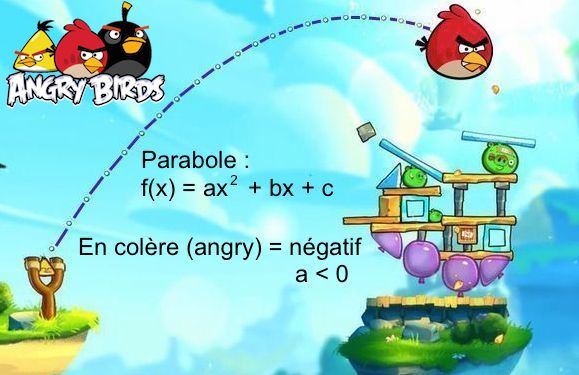
\includegraphics[scale=0.25]{01-01-03}~\\[1.5cm]

    \textsc{\LARGE 1ère spécialité maths}\\[1.5cm]
    
    
\includegraphics[scale=0.9]{logo fond transparent}~\\[1cm]

    %\textsc{\Large Rapport de stage 1A}\\[1.5cm]

    % Title
    \HRule \\[0.4cm]
    { \huge \bfseries Cours de Mathématiques\\[0.4cm] }

    \HRule \\[2cm]
    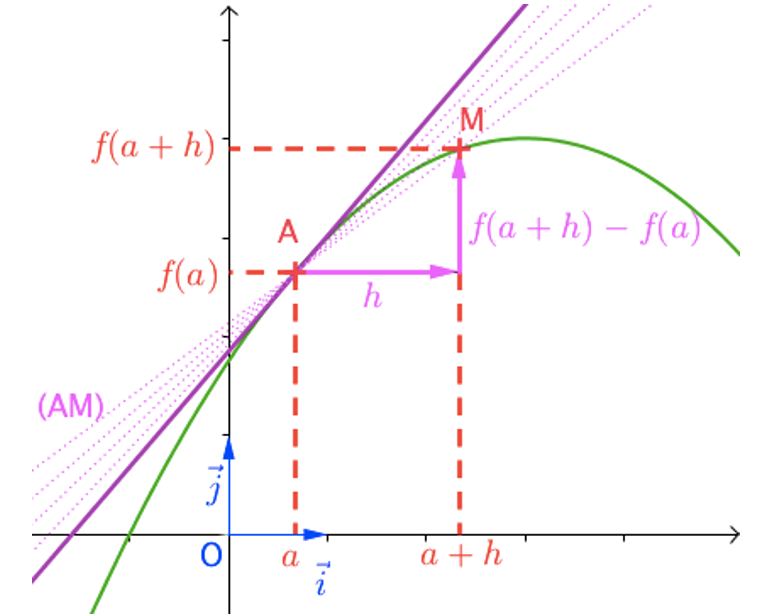
\includegraphics[scale=0.45]{01-05-Img04}
    \\[2cm]

    % Author and supervisor
    \begin{minipage}{0.4\textwidth}
      \begin{flushleft} \large
        Cours de M. Buisson
      \end{flushleft}
    \end{minipage}
    \begin{minipage}{0.45\textwidth}
      \begin{flushright} \large
        Lycée Notre-Dame de Bel Air - Tarare
      \end{flushright}
    \end{minipage}

    \vfill
    
    \vfill

    % Bottom of the page
    {\large Année scolaire 2024-2025}

  \end{center}
  \end{sffamily}
\end{titlepage}

\tableofcontents
\thispagestyle{fancy}

\input{1.01 - Fonctions de référence/1.01.01-Polynome-content}
\chapter{Trigonométrie}
\thispagestyle{fancy}

\vspace{-0.5cm}
\section{Cercle trigonométrique et radian}

\subsection{Le cercle trigonométrique}

    \begin{minipage}{0.65\linewidth}
        \begin{bdefi}
            Sur un cercle, on appelle \grasInDef{sens direct, sens positif ou sens trigonométrique} le sens contraire des aiguilles d'une montre.
        \end{bdefi}
    
        \begin{bdefi}
            Dans le plan muni d'un repère orthonormé \Rij  et orienté dans le sens direct, le \grasInDef{cercle trigonométrique} est le cercle de centre O et de rayon 1.
        \end{bdefi}
    \end{minipage} \hfill
    \begin{minipage}[c]{0.35\linewidth}
        \psset{xunit=2cm,yunit=2cm,algebraic=true,dimen=middle,dotstyle=o,dotsize=5pt 0,linewidth=0.8pt,arrowsize=3pt 2,arrowinset=0.25}
        \begin{pspicture*}(-1.2,-1.2)(1.8,1.5)
        \psaxes[labelFontSize=\scriptstyle,xAxis=true,yAxis=true,labels=none,Dx=1,Dy=1,ticksize=-2pt 0,subticks=1]{->}(0,0)(-1.2,-1.2)(1.8,1.5)
        \pscircle[linewidth=0.8pt,linecolor=ForestGreen](0.,0.){2}
        \parametricplot[linewidth=1.2pt,linecolor=red]{0.2836313716099023}{1.2179063232586265}{1.*1.3698332060350076*cos(t)+0.*1.3698332060350076*sin(t)+0.|0.*1.3698332060350076*cos(t)+1.*1.3698332060350076*sin(t)+0.}
        \rput[tl](1.01,1.1){\footnotesize \red{Sens Direct}}
        \psline[linewidth=1.2pt,linecolor=blue]{->}(0.,0.)(1.,0.)
        \psline[linewidth=1.2pt,linecolor=blue]{->}(0.,0.)(0.,1.)
        \rput[tl](0.41,-0.1){\footnotesize $\blue{\vv{i}}$}
        \rput[tl](-0.17,0.55){\footnotesize $\blue{\vv{j}}$}
        \psline[linewidth=2.pt,linecolor=red](0.4734296463271147,1.2854210914461963)(0.5317198467755907,1.2004882024713655)
        \psline[linewidth=2.pt,linecolor=red](0.4734296463271147,1.2854210914461963)(0.5924995182352584,1.2882810612464408)
        \rput[tl](0.8,0.9){\Large \red{+}}
        \begin{scriptsize}
        %\psdots[dotsize=4pt 0,dotstyle=*,linecolor=darkgray](0.,0.)
        \rput[bl](-0.17737632025386682,-0.1434178664701735){O}
        \end{scriptsize}
        \end{pspicture*}
        %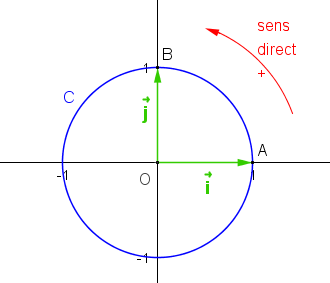
\includegraphics[scale=0.7]{01-02-01.png}
    \end{minipage}
    \vspace{-0.5cm}
    \subsection{Enroulement d'une droite autour du cercle trigonométrique}
    
    \begin{minipage}{0.65\linewidth}
        Dans un repère orthonormé \Rij), on considère le cercle trigonométrique et une droite (AC) tangente au cercle en A et orientée telle que $(A ; \vv{j})$ soit un repère de la droite.\\
        Si l'on \guillemets{enroule} la droite autour du cercle, on associe à tout point $N$ d'abscisse $x$ de la droite orientée un unique point $M$ du cercle.\\
        La longueur de l'arc $\wideparen{AM}$ est ainsi égale à la longueur AN.
    \end{minipage} \hfill
    \begin{minipage}[c]{0.35\linewidth}
        \psset{xunit=1.5cm,yunit=1.5cm,algebraic=true,dimen=middle,dotstyle=o,dotsize=5pt 0,linewidth=0.8pt,arrowsize=3pt 2,arrowinset=0.25}
        \begin{pspicture*}(-1.35,-1.2)(1.35,2.2)
        \psaxes[labelFontSize=\scriptstyle,xAxis=true,yAxis=true,labels=none,Dx=1.,Dy=1.,ticksize=-2pt 0,subticks=2]{->}(0,0)(-1.35,-1.2)(1.35,2.2)
        \pscircle[linewidth=0.8pt,linecolor=ForestGreen](0.,0.){1.5}
        \parametricplot[linewidth=1.2pt,linecolor=red]{2.3320450984702887}{2.872851867759325}{1.*1.2850666792859502*cos(t)+0.*1.2850666792859502*sin(t)+0.|0.*1.2850666792859502*cos(t)+1.*1.2850666792859502*sin(t)+0.}
        \psline[linewidth=0.8pt,linecolor=blue]{->}(0.,0.)(1.,0.)
        \psline[linewidth=0.8pt,linecolor=blue]{->}(0.,0.)(0.,1.)
        \rput[tl](0.41,-0.1){\footnotesize $\blue{\vv{i}}$}
        \rput[tl](-0.17,0.55){\footnotesize $\blue{\vv{j}}$}
        \psline[linewidth=1.2pt,linecolor=red](-1.238940501289754,0.34120786109776535)(-1.1566043604374026,0.4103524734956868)
        \psline[linewidth=1.2pt,linecolor=red](-1.238940501289754,0.34120786109776535)(-1.264657109699034,0.4373656608110946)
        \rput[tl](-1.3,0.8){\Large \red{+}}
        \psline[linewidth=1.2pt,linecolor=red](1.,-1.2)(1.,2.2)
        \parametricplot[linewidth=0.8pt,linestyle=dashed,dash=2pt 2pt]{1.5413461266504365}{2.7472202756000637}{1.*1.5815250404268189*cos(t)+0.*1.5815250404268189*sin(t)+0.9534305034388083|0.*1.5815250404268189*cos(t)+1.*1.5815250404268189*sin(t)+0.2544588540208172}
        \psline[linewidth=0.8pt](-0.5066933483806594,0.862126354258351)(-0.514999515949157,1.0228852089153582)
        \psline[linewidth=0.8pt](-0.5066933483806594,0.862126354258351)(-0.3974463572218636,0.9694519549484067)
        \parametricplot[linewidth=2.pt,linecolor=ForestGreen]{0.0}{2.1021413143570626}{1.*1.*cos(t)+0.*1.*sin(t)+0.|0.*1.*cos(t)+1.*1.*sin(t)+0.}
        \psline[linewidth=1.2pt]{->}(0.,0.)(-0.5066933483806594,0.862126354258351)
        \psline[linewidth=2.pt,linecolor=red](1.,0.)(1.,1.8352981043834493)
        \begin{scriptsize}
        \psdots[dotsize=4pt 0,dotstyle=*,linecolor=darkgray](0.,0.)
        \rput[bl](-0.2798931984945702,-0.22745293391130536){\darkgray{$O$}}
        %\psdots[dotsize=4pt 0,dotstyle=*,linecolor=darkgray](1.,0.)
        \rput[bl](1.0452514998858287,0.08245993909701295){\darkgray{$A$}}
        \psdots[dotstyle=x](-0.5066933483806594,0.862126354258351)
        \rput[bl](-0.75,0.95){$M$}
        \psdots[dotstyle=x](1.,1.8352981043834493)
        \rput[bl](0.6,1.9){N(x)}
        \end{scriptsize}
        \end{pspicture*}
        %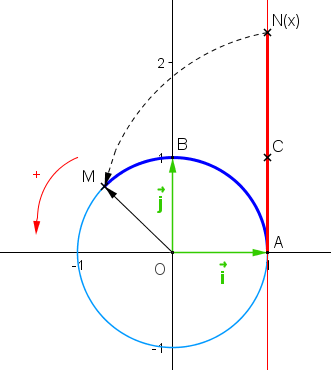
\includegraphics[scale=0.55]{01-02-02.png}
    \end{minipage}
    
    \vspace{-1cm}
    \subsection{Le radian}
    
    La longueur du cercle trigonométrique est égale à $2\pi$.\\
    En effet, son rayon est 1 donc $P = 2\pi R = 2\pi \times 1 = 2\pi$\\
    Ainsi, à un tour complet sur le cercle, on peut faire correspondre le nombre réel $2\pi$.\\
    On définit alors une nouvelle unité d'angle : le radian, tel qu'un tour complet mesure 360\degree ou $2\pi$ radians.

    \begin{bdefi}
        On appelle \grasInDef{radian}, noté rad, la mesure de l'angle au centre qui intercepte un arc de longueur 1 du cercle.
        \begin{center}
        \psset{xunit=0.5cm,yunit=0.5cm,algebraic=true,dimen=middle,dotstyle=o,dotsize=5pt 0,linewidth=2.pt,arrowsize=3pt 2,arrowinset=0.25}
        \begin{pspicture*}(-3.5,-3.5)(3.5,3.5)
        \pscircle[linewidth=0.8pt](0.,0.){1.5}
        \pscustom[linewidth=1.2pt,linecolor=ForestGreen,fillcolor=ForestGreen,fillstyle=solid,opacity=0.1]{
        \parametricplot{0.0}{1.0077885168662493}{0.6*cos(t)+0.|0.6*sin(t)+0.}
        \lineto(0.,0.)\closepath}
        \psline[linewidth=1.2pt,linecolor=red](0.,0.)(3.,0.)
        \parametricplot[linewidth=1.2pt,linecolor=red]{0.0}{1.0077885168662493}{1.*3.*cos(t)+0.*3.*sin(t)+0.|0.*3.*cos(t)+1.*3.*sin(t)+0.}
        \psline[linewidth=1.2pt](0.,0.)(1.6011965208465855,2.5369607213413436)
        \begin{scriptsize}
        \psdots[dotsize=4pt 0,dotstyle=*,linecolor=darkgray](0.,0.)
        \rput[bl](-0.52,-0.42){\darkgray{$O$}}
        \rput[bl](1.48,-0.42){\red{1}}
        \rput[bl](2.74,1.58){\red{1}}
        \rput[bl](0.64,0.2){\textcolor{ForestGreen}{1 rad}}
        \end{scriptsize}
        \end{pspicture*}
        %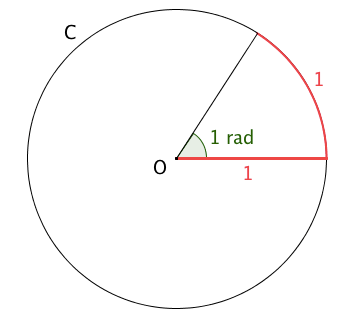
\includegraphics[scale=0.35]{01-02-03.png}
        \end{center}
    \end{bdefi}
    
    \subsection{Correspondance degrés et radians}
    
    Ainsi, à $2\pi$ radians (tour complet), on fait correspondre un angle de $360\degree$.\\
    Par proportionnalité, on obtient les correspondances suivantes :\\
    \ \\
    \begin{tabular}{ | Xc | Xc | Xc | Xc | Xc | Xc | Xc | Xc |}
         \hline			
           \rowcolor{NavyBlue!55!white}Angle en degrée($\degree$)  & 0 & 30 & 45 & 60 & 90 & 180 & 360 \\ \hline
           \rowcolor{NavyBlue!25!white}Angle en radian & $0$ & $\dfrac{\pi}{6}$ & $\dfrac{\pi}{4}$ & $\dfrac{\pi}{3}$ & $\dfrac{\pi}{2}$ & $\pi$ & $2\pi$ \\
         \hline  
    \end{tabular}
    
    \begin{bmethodet}{Passer des degrés aux radians et réciproquement}
        \grasInMet{Enoncé :}
        \begin{enumMet}
            \item Donner la mesure en radians de l'angle $\alpha$ de mesure $33\degree$.
            \item Donner la mesure en degrés de l'angle $\beta$ de mesure $\dfrac{3\pi}{8}$ rad.
        \end{enumMet}
        \grasInMet{Réponse :}\\
            \begin{tabular}{ | Xc | Xc | Xc |}
             \hline			
               $2\pi$  & $\alpha$ & $\dfrac{3\pi}{8}$ \\ \hline
               $360\degree$ & $33\degree$ & $\beta$ \\
             \hline  
            \end{tabular}
        \begin{enumMet}
            \item $\alpha = 33\times \dfrac{2\pi}{360}=\dfrac{11\pi}{60}$
            \item $\beta = \dfrac{3\pi}{8}\times\dfrac{360}{2\pi}=67,5\degree$
        \end{enumMet}
    \end{bmethodet}
    
\section{Mesure d'un angle orienté}

    \subsection{Plusieurs enroulements de la droite}
        \begin{minipage}{0.55\linewidth}
            A plusieurs points de la droite orientée on peut faire correspondre un même point du cercle. La droite orientée peut en effet s'enrouler plusieurs fois autour du cercle dans un sens et dans l'autre.\\
            \begin{bexemples}
            \begin{itemEx}
                \item Ci-contre, les points $N$ et $P$ d'abscisses $\dfrac{3\pi}{4}$ et $-\dfrac{5\pi}{4}$ correspondent tous les deux au point $M$.\\ 
                En effet : $\dfrac{3\pi}{4} -2\pi= -\dfrac{5\pi}{4}$
                \item On pourrait poursuivre le processus dans l'autre sens en effectuant 1, 2, 3, ... tours successifs.\\ 
                % Ainsi, les points d'abscisses $\dfrac{3\pi}{4}$ et $\dfrac{19\pi}{4}$ correspondent au point $M$.\\ 
                % En effet : $\dfrac{3\pi}{4} +4\pi= \dfrac{19\pi}{4}$.
            \end{itemEx}
        \end{bexemples}
        \end{minipage} \hfill
        \begin{minipage}{0.4\linewidth}
            \begin{center}
                \newrgbcolor{qqzzqq}{0. 0.6 0.}
                \newrgbcolor{xfqqff}{0.4980392156862745 0. 1.}
                \psset{xunit=1.0cm,yunit=1.0cm,algebraic=true,dimen=middle,dotstyle=o,dotsize=8pt 0,linewidth=0.8pt,arrowsize=3pt 2,arrowinset=0.25}
                \begin{pspicture*}(-2.,-4.5)(2.5,2.3)
                \psaxes[labelFontSize=\scriptstyle,xAxis=true,yAxis=true,labels=none,Dx=1.,Dy=1.,ticksize=-2pt 0,subticks=2]{->}(0,0)(-2.,-4.5)(2.5,2.3)
                \pspolygon[linewidth=1.2pt,fillcolor=black,fillstyle=solid,opacity=1](-0.5066933483806594,0.862126354258351)(-0.42451275812065586,0.9172810429953469)(-0.5054792770152563,0.957764302442647)
                \pspolygon[linewidth=1.2pt,fillcolor=black,fillstyle=solid,opacity=1](-0.5066933483806594,0.862126354258351)(-0.5521299533927227,0.7798135579819784)(-0.6067341821145836,0.8400182204189017)
                \pscircle[linewidth=0.8pt,linecolor=qqzzqq](0.,0.){1.}
                \parametricplot[linewidth=1.2pt,linecolor=red]{2.3320450984702887}{2.872851867759325}{1.*1.2850666792859502*cos(t)+0.*1.2850666792859502*sin(t)+0.|0.*1.2850666792859502*cos(t)+1.*1.2850666792859502*sin(t)+0.}
                \psline[linewidth=1.pt,linecolor=blue]{->}(0.,0.)(1.,0.)
                \psline[linewidth=1.pt,linecolor=blue]{->}(0.,0.)(0.,1.)
                \rput[tl](0.422451499927241,0.1348897567913225){$\blue{\vec{i}}$}
                \rput[tl](-0.18368461700829827,0.7042903514883441){$\blue{\vec{j}}$}
                \psline[linewidth=1.2pt,linecolor=red](-1.238940501289754,0.34120786109776535)(-1.1566043604374026,0.4103524734956868)
                \psline[linewidth=1.2pt,linecolor=red](-1.238940501289754,0.34120786109776535)(-1.264657109699034,0.4373656608110946)
                \rput[tl](-1.1939114785675304,0.9063357238001903){\red{+}}
                \psline[linewidth=0.8pt](1.,-4.5)(1.,2.3)
                \parametricplot[linewidth=1.2pt,linestyle=dashed,dash=2pt 2pt]{1.5413461266504365}{2.7472202756000637}{1.*1.5815250404268189*cos(t)+0.*1.5815250404268189*sin(t)+0.9534305034388083|0.*1.5815250404268189*cos(t)+1.*1.5815250404268189*sin(t)+0.2544588540208172}
                \parametricplot[linewidth=1.2pt,linecolor=red]{0.0}{2.1021413143570626}{1.*1.*cos(t)+0.*1.*sin(t)+0.|0.*1.*cos(t)+1.*1.*sin(t)+0.}
                \psline[linewidth=1.2pt]{->}(0.,0.)(-0.5066933483806594,0.862126354258351)
                \psline[linewidth=1.2pt,linecolor=red](1.,0.)(1.,1.8352981043834493)
                \psline[linewidth=1.2pt,linecolor=xfqqff](1.,0.)(1.,-3.74336104493671)
                \parametricplot[linewidth=1.2pt,linecolor=xfqqff]{-4.181043992822524}{0.0}{1.*1.*cos(t)+0.*1.*sin(t)+0.|0.*1.*cos(t)+1.*1.*sin(t)+0.}
                \parametricplot[linewidth=1.2pt,linestyle=dashed,dash=2pt 2pt]{2.1610272289783277}{4.754511813416839}{1.*2.5167627116062086*cos(t)+0.*2.5167627116062086*sin(t)+0.8940181721833393|0.*2.5167627116062086*cos(t)+1.*2.5167627116062086*sin(t)+-1.2288307908526448}
                \psline[linewidth=1.2pt](-0.5066933483806594,0.862126354258351)(-0.42451275812065586,0.9172810429953469)
                \psline[linewidth=1.2pt](-0.42451275812065586,0.9172810429953469)(-0.5054792770152563,0.957764302442647)
                \psline[linewidth=1.2pt](-0.5054792770152563,0.957764302442647)(-0.5066933483806594,0.862126354258351)
                \psline[linewidth=1.2pt](-0.5066933483806594,0.862126354258351)(-0.5521299533927227,0.7798135579819784)
                \psline[linewidth=1.2pt](-0.5521299533927227,0.7798135579819784)(-0.6067341821145836,0.8400182204189017)
                \psline[linewidth=1.2pt](-0.6067341821145836,0.8400182204189017)(-0.5066933483806594,0.862126354258351)
                \begin{scriptsize}
                %\psdots[dotsize=1pt 0,dotstyle=*,linecolor=darkgray](0.,0.)
                \rput[bl](-0.47756879491643855,-0.37940755454792274){\darkgray{$O$}}
                %\psdots[dotsize=1pt 0,dotstyle=*,linecolor=darkgray](1.,0.)
                \rput[bl](1.0653231391012978,0.15325751791058126){\darkgray{$A$}}
                \psdots[dotstyle=x](-0.5066933483806594,0.862126354258351)
                \rput[bl](-0.7347174505860613,1.071645573873519){$M$}
                \psdots[dotstyle=x](1.,1.8352981043834493)
                \rput[bl](1.17,1.53){$N\left(\dfrac{3\pi}{4}\right)$}
                \psdots[dotstyle=x](1.,-3.74336104493671)
                \rput[bl](1.0653231391012978,-3.557030228179688){$P\left(-\dfrac{5\pi}{4}\right)$}
                \end{scriptsize}
                \end{pspicture*}
                %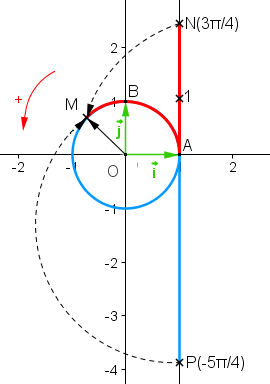
\includegraphics[scale=0.65]{01-02-04.png}
            \end{center}
        \end{minipage}
        
        
        \begin{bmethodet}{Placer un point sur le cercle trigonométrique}
            \grasInMet{Enoncé :}
            \begin{enumMet}
                \item Placer sur le cercle trigonométrique, le point $M$ tel que l'angle $(\vv{i}  ;\vv{OM} )$ mesure $\dfrac{9\pi}{4}$ rad.
                \item Placer sur le cercle trigonométrique, le point $N$ tel que l'angle $(\vv{i}  ;\vv{ON} )$ mesure $\dfrac{8\pi}{3}$ rad.
            \end{enumMet}
            \grasInMet{Réponse :}\\
                \begin{minipage}{0.55\linewidth}
                    \begin{enumMet}
                        \item $\dfrac{9\pi}{4}=\dfrac{8\pi}{4}+\dfrac{\pi}{4}=2\pi +\dfrac{\pi}{4}$.\\
                        Le point $M$ se trouve donc sur le cercle trigonométrique tel que l'angle $(\vv{i}  ;\vv{OM} )$ mesure $\dfrac{\pi}{4}$ rad.
                        \item $\dfrac{8\pi}{6}=\dfrac{6\pi}{3}+\dfrac{2\pi}{3}=2\pi +\dfrac{2\pi}{3}$.\\
                        Le point $N$ se trouve donc sur le cercle trigonométrique tel que l'angle $(\vv{i}  ;\vv{ON} )$ mesure $\dfrac{2\pi}{3}$ rad.
                    \end{enumMet}
                \end{minipage} \hfill
                \begin{minipage}{0.45\linewidth}
                    \begin{center}
                        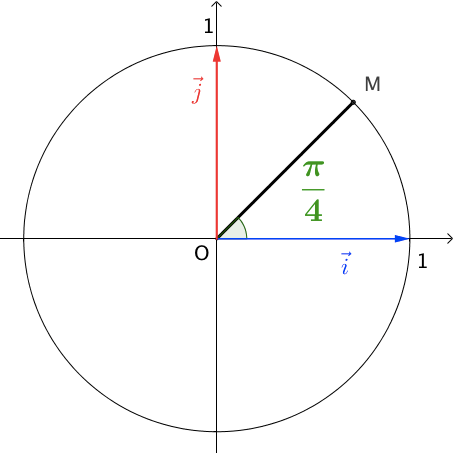
\includegraphics[scale=0.3]{01-02-05.png}
                        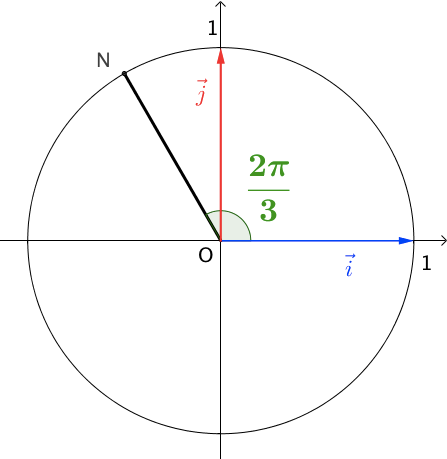
\includegraphics[scale=0.3]{01-02-06.png}
                    \end{center}
                \end{minipage}
        \end{bmethodet}
        
        
        
            
        
    \subsection{Mesure principale d'un angle orienté }
    
        On a vu qu'un angle possède plusieurs mesures.\\
        Si $\theta$ est une mesure de l'angle  $(\vv{i}  ;\vv{OM} )$ alors tout angle de la forme $\theta+k\times2\pi$, avec $k\in \Z$, est une mesure de l'angle $(\vv{i}  ;\vv{OM} )$.\\
        On dit que l'angle $(\vv{i}  ;\vv{OM} )$ est égal à $\theta$ modulo $2\pi$.
        
        \begin{bdefi}
            La \grasInDef{mesure principale d'un angle orienté} est la mesure, qui parmi toutes les autres, se situe dans l'intervalle $\intervOF{-\pi}{\pi}$.
        \end{bdefi}
        
        \begin{bexemple}
            Une mesure d'un angle orienté est $\dfrac{7\pi}{4}$.\\
            D'autres mesures sont : $\dfrac{7\pi}{4}-2\pi$; $\dfrac{7\pi}{4}-4\pi$; $\dfrac{7\pi}{4}-6\pi$; ... soit : $-\dfrac{\pi}{4}$ ; $-\dfrac{9\pi}{4}$ ; $-\dfrac{17\pi}{4}$ ; ...\\
            $-\dfrac{\pi}{4}$ est la mesure principale de cet angle orienté car c'est la seule comprise entre $–\pi$ exclu et $\pi$.
        \end{bexemple}
        
        \begin{bmethodet}{Donner la mesure principale d'un angle}
            \grasInMet{Enoncé :}\\
            Donner la mesure principale de l'angle $\dfrac{27\pi}{4}$.\\ 
            \grasInMet{Réponse :}\\
                On choisit un multiple de 4 proche de 27, soit 28 :\\
                $\dfrac{27\pi}{4}=\dfrac{28\pi}{4}-\dfrac{\pi}{4}=7\pi-\dfrac{\pi}{4}$\\
                Dans  $7\pi$, on fait apparaître un multiple de $2\pi$, soit $6\pi$ :\\
                $\dfrac{27\pi}{4}=6\pi+\pi-\dfrac{\pi}{4}=6\pi+\dfrac{4\pi}{4}-\dfrac{\pi}{4}=6\pi+\dfrac{3\pi}{4}$\\
                $6\pi$ correspond à 3 tours entiers.\\
                $\dfrac{3\pi}{4}$ est bien compris entre $–\pi$ exclu et $\pi$.\\
                La mesure principale de $\dfrac{27\pi}{4}$ est $\dfrac{3\pi}{4}$. 
        \end{bmethodet}
\vspace{-1cm}
\section{Cosinus et sinus d'un angle}
    \subsection{Définitions}
    
        \begin{minipage}{0.55\linewidth}
            Dans le plan muni d'un repère orthonormé \Rij et orienté dans le sens direct, on considère un cercle trigonométrique de centre $O$.\\
            Pour tout nombre réel $x$, considérons le point $N$ de la droite orientée d'abscisse $x$.\\ 
            À ce point, on fait correspondre un point $M$ sur le cercle trigonométrique.\\
            On appelle $H$ et $K$ les pieds respectifs des perpendiculaires à l'axe des abscisses et à l'axe des ordonnées passant par $M$.
        \end{minipage} \hfill
        \begin{minipage}{0.45\linewidth}
            \begin{center}
                \newrgbcolor{xfqqff}{0.4980392156862745 0. 1.}
                \newrgbcolor{qqzzqq}{0. 0.6 0.}
                \psset{xunit=2cm,yunit=2cm,algebraic=true,dimen=middle,dotstyle=o,dotsize=8pt 0,linewidth=0.8pt,arrowsize=3pt 2,arrowinset=0.25}
                \begin{pspicture*}(-1.5,-1.2)(1.5,1.2)
                \psaxes[labelFontSize=\scriptstyle,xAxis=true,yAxis=true,labels=none,Dx=1,Dy=1,ticksize=-2pt 0,subticks=1]{->}(0,0)(-1.5,-1.2)(1.5,1.2)
                \pspolygon[linewidth=1.2pt,linecolor=red,fillcolor=red,fillstyle=solid,opacity=1](0.40977974882738943,0.4381983185914975)(0.41741048167754885,0.4184481865087321)(0.4281832809954209,0.43191418565607215)
                \pscircle[linewidth=0.8pt](0.,0.){2}
                \parametricplot[linewidth=1.2pt,linecolor=red]{2.3320450984702887}{2.872851867759325}{1.*1.2850666792859502*cos(t)+0.*1.2850666792859502*sin(t)+0.|0.*1.2850666792859502*cos(t)+1.*1.2850666792859502*sin(t)+0.}
                \psline[linewidth=1.2pt,linecolor=blue]{->}(0.,0.)(1.,0.)
                \psline[linewidth=1.2pt,linecolor=blue]{->}(0.,0.)(0.,1.)
                \rput[tl](0.7,-0.05){\scriptsize $\blue{\vv{i}}$}
                \rput[tl](-0.2,0.88){\scriptsize $\blue{\vv{j}}$}
                \psline[linewidth=1.2pt,linecolor=red](-1.238940501289754,0.34120786109776535)(-1.1566043604374026,0.4103524734956868)
                \psline[linewidth=1.2pt,linecolor=red](-1.238940501289754,0.34120786109776535)(-1.264657109699034,0.4373656608110946)
                \rput[tl](-1.22,0.74){\red{+}}
                \psline[linewidth=0.8pt](1.,-1.2)(1.,1.2)
                \parametricplot[linewidth=0.8pt,linestyle=dashed,dash=1pt 1pt]{1.7070104914828212}{1.989170336710919}{1.*1.1703098632121625*cos(t)+0.*1.1703098632121625*sin(t)+1.1589202721830498|0.*1.1703098632121625*cos(t)+1.*1.1703098632121625*sin(t)+-0.3393763856576485}
                \parametricplot[linewidth=1.2pt,linecolor=red]{0.0}{0.8183148200277329}{1.*1.*cos(t)+0.*1.*sin(t)+0.|0.*1.*cos(t)+1.*1.*sin(t)+0.}
                \psline[linewidth=1.2pt]{->}(0.,0.)(0.6834523503170895,0.7299951265906138)
                \psline[linewidth=1.2pt,linecolor=red](1.,0.)(1.,0.8200931150283057)
                \parametricplot[linewidth=1.2pt,linecolor=red]{0.0}{0.8188989562169464}{1.*0.6*cos(t)+0.*0.6*sin(t)+0.|0.*0.6*cos(t)+1.*0.6*sin(t)+0.}
                \psline[linewidth=1.2pt,linecolor=red](0.40977974882738943,0.4381983185914975)(0.41741048167754885,0.4184481865087321)
                \psline[linewidth=1.2pt,linecolor=red](0.41741048167754885,0.4184481865087321)(0.4281832809954209,0.43191418565607215)
                \psline[linewidth=1.2pt,linecolor=red](0.4281832809954209,0.43191418565607215)(0.40977974882738943,0.4381983185914975)
                \psline[linewidth=0.8pt,linestyle=dashed,dash=1pt 1pt](0.6834523503170895,0.7299951265906138)(0.,0.7283487195713757)
                \psline[linewidth=0.8pt,linestyle=dashed,dash=1pt 1pt](0.6834523503170895,0.7299951265906138)(0.684411097342735,0.)
                \psline[linewidth=1.2pt,linecolor=xfqqff](0.,0.)(0.,0.7283487195713757)
                \psline[linewidth=1.2pt,linecolor=qqzzqq](0.,0.)(0.684411097342735,0.)
                \begin{scriptsize}
                \psdots[dotsize=2pt 0,dotstyle=*,linecolor=darkgray](0.,0.)
                \rput[bl](-0.15,-0.15){\darkgray{$O$}}
                \psdots[dotsize=2pt 0,dotstyle=*,linecolor=darkgray](1.,0.)
                \rput[bl](1.0170341702650048,0.03160536668364699){\darkgray{$A$}}
                \psdots[dotstyle=x](0.6834523503170895,0.7299951265906138)
                \rput[bl](0.6367693438651923,0.7723295597749434){$M$}
                \psdots[dotstyle=x](1.,0.8200931150283057)
                \rput[bl](1.0170341702650048,0.8594735824915666){N(x)}
                \rput[bl](0.573391872798557,0.26530979124186355){\red{x}}
                \psdots[dotsize=2pt 0,dotstyle=*](0.,0.7283487195713757)
                \rput[bl](0.014877909023832495,0.7683684678332788){$K$}
                \psdots[dotsize=2pt 0,dotstyle=*](0.684411097342735,0.)
                \rput[bl](0.7001468149318277,0.03952755056697636){$H$}
                \rput[bl](-0.4,0.35){\xfqqff{sin(x)}}
                \rput[bl](0.24,-0.15){\qqzzqq{cos(x)}}
                \end{scriptsize}
                \end{pspicture*}
                %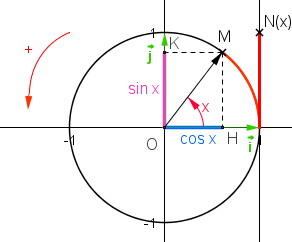
\includegraphics[scale=0.8]{01-02-07.png}
            \end{center}
        \end{minipage}
        
        \begin{bdefis}
            \begin{itemDef}
                \item Le \grasInDef{cosinus} du nombre réel $x$ est l'abscisse de $M$ et on note $\cos x$.
                \item Le \grasInDef{sinus} du nombre réel $x$ est l'ordonnée de $M$ et on note $\sin x$.
            \end{itemDef}
        \end{bdefis}
        
    \subsection{Propriétés}
        \begin{bprops}
            \begin{itemProp}
                \item $-1\leqslant \sin x \leqslant 1$ et $-1\leqslant \cos x \leqslant 1$.
                \item $\cos^2 x + \sin^2 x = 1$.
                \item $\sin(-x)=-\sin x$ et $\cos(-x)=\cos x$
                \item $\cos x= \cos(x+2k\pi)$ où $k$ entier relatif.
                \item $\sin x= \sin(x+2k\pi)$ où $k$ entier relatif.
            \end{itemProp}
        \end{bprops}
        
        \begin{brmq}
            $(\sin x)^2$, par exemple, se note $\sin^2 x$
        \end{brmq}
        
    \subsection{Valeurs remarquables des fonctions sinus et cosinus}
    
        \begin{center}
            \begin{tabular}{ | Xc | Xc | Xc | Xc | Xc | Xc | Xc |}
                 \hline			
                   \rowcolor{NavyBlue!55!white}$x$  & $0$ & $\dfrac{\pi}{6}$ & $\dfrac{\pi}{4}$ & $\dfrac{\pi}{3}$ & $\dfrac{\pi}{2}$ & $\pi$ \\ \hline
                   \rowcolor{NavyBlue!25!white}$\cos x$ & $1$ & $\dfrac{\sqrt 3}{2}$ & $\dfrac{\sqrt 2}{2}$ & $\dfrac{1}{2}$ & $0$ & $-1$ \\ \hline
                   \rowcolor{NavyBlue!25!white}$\sin x$ & $0$ & $\dfrac{1}{2}$ & $\dfrac{\sqrt 2}{2}$ & $\dfrac{\sqrt 3}{2}$ & $1$ & $0$ \\
                 \hline  
            \end{tabular}
        \end{center}
    
    \subsection{Cosinus et sinus d'angles associés}
    
        \begin{bprops}
            Pour tout nombre réel $x$, on a :
            \begin{enumProp}
                \item $\cos(\pi+x)=-\cos(x)$ et $\sin(\pi+x)=-\sin(x)$.
                \item $\cos(\pi-x)=-\cos(x)$ et $\sin(\pi-x)=\sin(x)$.
                \item $\cos(\dfrac{\pi}{2}+x)=-\sin(x)$ et $\sin(\dfrac{\pi}{2}+x)=\cos(x)$.
                \item $\cos(\dfrac{\pi}{2}-x)=\sin(x)$ et $\sin(\dfrac{\pi}{2}-x)=\cos(x)$.
            \end{enumProp}
        \end{bprops}
        
        \begin{bdemo}
            \begin{multicols}{2}
                [
                Par symétries, on démontre les résultats :
                ]
                \begin{enumDem}
                    \item \ \\ 
                    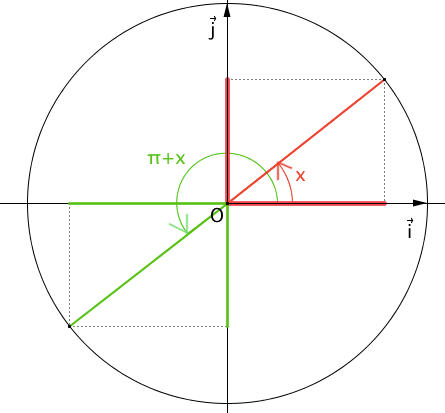
\includegraphics[scale=0.35]{01-02-12.png}
                    \item \ \\ 
                    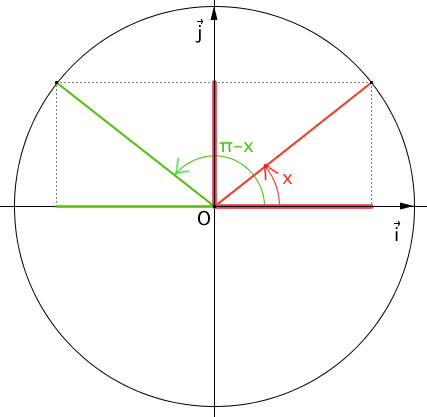
\includegraphics[scale=0.35]{01-02-13.png}
                    \item \ \\ 
                    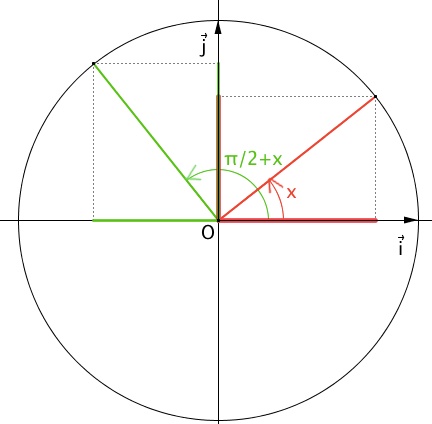
\includegraphics[scale=0.35]{01-02-14.png}
                    \item \ \\ 
                    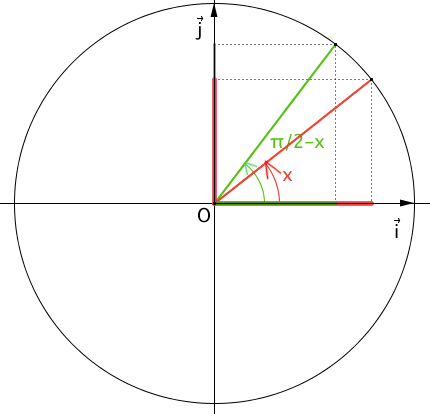
\includegraphics[scale=0.35]{01-02-15.png}
                \end{enumDem}
            \end{multicols}
            
        \end{bdemo}
        
%	\begin{bmethodet}[Résoudre une équation trigonométrique]
%			\grasInMet{Enoncé :}\\
%			\begin{enumMet}
%			\item Résoudre sur $[3\pi;5\pi]$ l'équation $\cos x=\dfrac{\sqrt{3}}{2}$
%			\item Résoudre sur $\left[\dfrac{7\pi}{2};\dfrac{10\pi}{2}\right]$ l'équation $\sin x=-\dfrac{1}{2}$
%			\end{enumMet}
%		\grasInMet{Réponse :}\\
%		\ \\
%		\begin{enumMet}
%		\begin{minipage}{0.65\linewidth}
%			\item On commence par étudier la solution dans l'intervalle\\ $]-\pi;\pi]$ (parmi les mesures principales de l'angle).\\
%			L'équation $\cos x=\dfrac{\sqrt{3}}{2}$ a pour solution :\\
%			$\begin{cases}
%			x_1 &=\dfrac{\pi}{6}\\
%			x_2 &=-\dfrac{\pi}{6}
%			\end{cases}$\\
%			On en déduit les solutions sur \R.\\
%			L'équation $\cos x=\dfrac{\sqrt{3}}{2}$ a pour solution ($k\in \Z$ ) :\\
%			$\begin{cases}
%				x_1 &=\dfrac{\pi}{6}+2k\pi\\
%				x_2 &=-\dfrac{\pi}{6}+2k\pi\
%			\end{cases}$\\
%			On teste différentes valeurs de $k$ pour trouver les valeurs qui appartiennent à l'intervalle souhaité $[3\pi;5\pi]$ (ou $\left[\dfrac{18\pi}{12};\dfrac{30\pi}{6}\right]$)\\
%			$k=1\quad \begin{cases}
%				x_1 &=\dfrac{\pi}{6}+2\pi=\dfrac{13\pi}{6}\notin\left[\dfrac{18\pi}{12};\dfrac{30\pi}{6}\right]\\
%				x_2 &=-\dfrac{\pi}{6}+2\pi=\dfrac{11\pi}{6}\notin\left[\dfrac{18\pi}{12};\dfrac{30\pi}{6}\right]
%			\end{cases}$\\
%			$k=2\quad \begin{cases}
%				x_1 &=\dfrac{\pi}{6}+4\pi=\dfrac{25\pi}{6}\in\left[\dfrac{18\pi}{12};\dfrac{30\pi}{6}\right]\\
%				x_2 &=-\dfrac{\pi}{6}+4\pi=\dfrac{23\pi}{6}\in\left[\dfrac{18\pi}{12};\dfrac{30\pi}{6}\right]
%			\end{cases}$\\
%			$k=3\quad \begin{cases}
%				x_1 &=\dfrac{\pi}{6}+6\pi=\dfrac{37\pi}{6}\notin\left[\dfrac{18\pi}{12};\dfrac{30\pi}{6}\right]\\
%				x_2 &=-\dfrac{\pi}{6}+6\pi=\dfrac{35\pi}{6}\notin\left[\dfrac{18\pi}{12};\dfrac{30\pi}{6}\right]
%			\end{cases}$\\
%			On peut maintenant conclure : $S=\left\{\dfrac{23\pi}{6};\dfrac{25\pi}{6}\right\}$
%		\end{minipage} \hfill
%			\begin{minipage}{0.35\linewidth}
%			\begin{center}
%				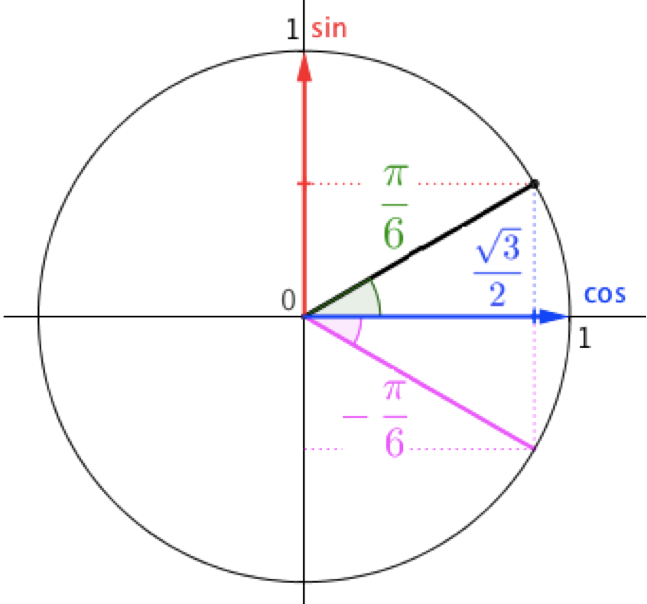
\includegraphics[scale=0.35]{01-02-16.png}
%			\end{center}
%		\end{minipage}
%			\begin{minipage}{0.65\linewidth}
%			\item On commence par étudier la solution dans l'intervalle\\ $]-\pi;\pi]$ (parmi les mesures principales de l'angle).\\
%			L'équation $\sin x=-\dfrac{1}{2}$ a pour solution :\\
%			$\begin{cases}
%			x_1 &=-\dfrac{\pi}{6}\\
%			x_2 &=-\dfrac{5\pi}{6}
%			\end{cases}$\\
%			On en déduit les solutions sur \R.\\
%			L'équation $\cos x=\dfrac{\sqrt{3}}{2}$ a pour solution ($k\in \Z$ ) :\\
%			$\begin{cases}
%				x_1 &=-\dfrac{\pi}{6}+2k\pi\\
%				x_2 &=-\dfrac{5\pi}{6}\pi\
%			\end{cases}$\\
%			On teste différentes valeurs de $k$ pour trouver les valeurs qui appartiennent à l'intervalle souhaité $\left[\dfrac{7\pi}{2};\dfrac{10\pi}{2}\right]$ (ou $\left[\dfrac{21\pi}{6};\dfrac{30\pi}{6}\right]$)\\
%			$k=1\quad \begin{cases}
%				x_1 &=-\dfrac{\pi}{6}+2\pi=\dfrac{11\pi}{6}\notin\left[\dfrac{21\pi}{6};\dfrac{30\pi}{6}\right]\\
%				x_2 &=-\dfrac{5\pi}{6}+2\pi=\dfrac{7\pi}{6}\notin\left[\dfrac{21\pi}{6};\dfrac{30\pi}{6}\right]
%			\end{cases}$\\
%			$k=2\quad \begin{cases}
%				x_1 &=\dfrac{\pi}{6}+4\pi=\dfrac{23\pi}{6}\in\left[\dfrac{21\pi}{6};\dfrac{30\pi}{6}\right]\\
%				x_2 &=-\dfrac{\pi}{6}+4\pi=\dfrac{19\pi}{6}\notin\left[\dfrac{21\pi}{6};\dfrac{30\pi}{6}\right]
%			\end{cases}$\\
%			$k=3\quad \begin{cases}
%				x_1 &=\dfrac{\pi}{6}+6\pi=\dfrac{35\pi}{6}\notin\left[\dfrac{21\pi}{6};\dfrac{30\pi}{6}\right]\\
%				x_2 &=-\dfrac{\pi}{6}+6\pi=\dfrac{31\pi}{6}\notin\left[\dfrac{21\pi}{6};\dfrac{30\pi}{6}\right]
%			\end{cases}$\\
%			On peut maintenant conclure : $S=\left\{\dfrac{23\pi}{6}\right\}$
%			
%			\end{minipage} \hfill
%		\begin{minipage}{0.35\linewidth}
%			\begin{center}
%			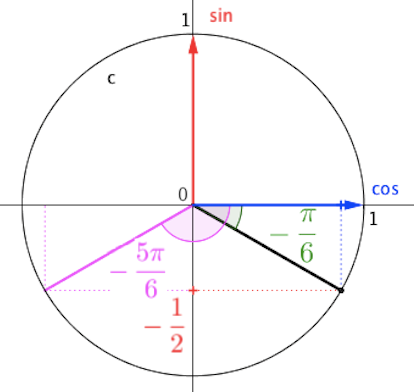
\includegraphics[scale=0.6]{01-02-17.png}
%			\end{center}
%		\end{minipage}
%			\end{enumMet}
%	\end{bmethodet}


\chapter{Équations du second degré}
\thispagestyle{fancy}

\section{Résolution d'une équation du second degré}

\subsection{Résoudre une équation à l'aide du discriminant}

    \begin{bdefi}
        Une \grasInDef{équation du second degré} est une équation de la forme $ax^2+bx+c=0$ où $a$, $b$ et $c$ sont des réels avec $a\neq 0$.\\
        Une solution de cette équation s'appelle une \grasInDef{racine} du trinôme $ax^2+bx+c$.
    \end{bdefi}
    
    \begin{bexemple}
        L'équation $3x^2-6x-2=0$ est une équation du second degré.
    \end{bexemple}
    
    \begin{brmq}
        Résoudre l'équation $3x^2-6x-2=0$ ou trouver les racines du trinôme $3x^2-6x-2$ sont deux énoncés identiques.
    \end{brmq}
        
    \begin{bdefi}
        On appelle \grasInDef{discriminant} du trinôme $ax^2+bx+c$, le nombre réel, noté $\Delta$, égal à $b^2-4ac$.
        $$\Delta = b^2-4ac$$
    \end{bdefi}
        
    \begin{bprop}
        Soit $\Delta$ le discriminant du trinôme $ax^2+bx+c$.\\
        \begin{itemProp}
            \item Si $\Delta < 0$ : L'équation $ax^2+bx+c=0$ n'a pas de solution réelle.
            \item Si $\Delta = 0$ : L'équation $ax^2+bx+c=0$ a une unique solution : $x_0= \dfrac{-b}{2a}$.
            \item Si $\Delta > 0$ : L'équation $ax^2+bx+c=0$ a deux solutions distinctes :\\
            \hspace*{3cm} $x_1= \dfrac{-b-\sqrt{\Delta}}{2a}$ \hspace*{0.5cm} et \hspace*{0.5cm} $x_2= \dfrac{-b+\sqrt{\Delta}}{2a}$
        \end{itemProp}         
    \end{bprop}
        
        
    \begin{bmethodet}{Résoudre une équation du second degré}
        \grasInMet{Enoncé :} Résoudre les équations suivantes : 
        \begin{enumMet}
            \item $2x^2-x-6=0$
            \item $2x^2-3x+\dfrac{9}{8}=0$.
            \item $x^2+3x+10=0$
        \end{enumMet}
        \grasInMet{Réponse :}\\
        \begin{enumMet}
            \item Calculons le discriminant de l'équation $2x^2-x-6=0$ :\\
            $a = 2$, $b = -1$ et $c = -6$ donc $\Delta = b^2-4ac = (-1)^2 - 4 \times 2 \times (-6) = 49$.\\
            Comme $\Delta > 0$, l'équation possède deux solutions distinctes :\\
            \hspace*{2cm} $x_1= \dfrac{-b-\sqrt{\Delta}}{2a}=\dfrac{-(-1)-\sqrt{49}}{2\times2}=-\dfrac{3}{2}$\\
            \hspace*{2cm} $x_2= \dfrac{-b+\sqrt{\Delta}}{2a}=\dfrac{-(-1)+\sqrt{49}}{2\times2}=2$
            \item Calculons le discriminant de l'équation $2x^2-3x+\dfrac{9}{8}=0$ :\\
            $a = 2$, $b = -3$ et $c = \dfrac{9}{8}$ donc $\Delta = b^2-4ac = (-3)^2 - 4 \times 2 \times \dfrac{9}{8} = 0$.\\
            Comme $\Delta = 0$, l'équation possède une solution unique :\\
            \hspace*{2cm} $x_0= -\dfrac{b}{2a}=-\dfrac{-3}{2\times2}=\dfrac{3}{4}$\\
            \item Calculons le discriminant de l'équation $x^2+3x+10=0$ :\\
            $a = 1$, $b = 3$ et $c = 10$ donc $\Delta = b^2-4ac = 3^2 - 4 \times 1 \times 10 = -31$.\\
            Comme $\Delta < 0$, l'équation ne possède pas de solution réelle.
        \end{enumMet}
    \end{bmethodet}
    
\subsection{Résoudre une équation à l'aide de la somme et du produit des racines}
    
    \begin{bprop}
        La somme $S$ et le produit $P$ des racines d'un polynôme du second degré de la forme $ax^2+bx+c$ sont donnés par : $S=- \dfrac{b}{a}$  et $P= \dfrac{c}{a}$. 
    \end{bprop}
    
    \begin{bdemo}
        \begin{itemDem}
            \item $S=x_1+x_2=\dfrac{-b-\sqrt{\Delta}}{2a}+\dfrac{-b+\sqrt{\Delta}}{2a}=\dfrac{-b-\sqrt{\Delta}-b+\sqrt{\Delta}}{2a}=\dfrac{-2b}{2a}=- \dfrac{b}{a}$
            \item $P=x_1\times x_2=\dfrac{-b-\sqrt{\Delta}}{2a}\times \dfrac{-b+\sqrt{\Delta}}{2a}=\dfrac{(-b-\sqrt{\Delta})\times(-b+\sqrt{\Delta})}{4a^2}=\dfrac{b^2-\Delta}{4a^2}=\dfrac{b^2-b^2+4ac}{4a^2}=\dfrac{c}{a}$
        \end{itemDem}
    \end{bdemo}
    
    \begin{bmethodet}{utiliser somme et produit pour trouver les 2 racines}
        \grasInMet{Enoncé :}\\
        Trouver les 2 racines du polynôme suivant : $2x^2+3x-5$\\
        \grasInMet{Réponse :}\\
        On a une solution évidente ($x_1=1$). Or la somme des 2 racines vaut $S=- \dfrac{b}{a}=-\dfrac{3}{2}$. Donc:\\
        $x_1+x_2=-\dfrac{3}{2} \iff 1+x_2=-\dfrac{3}{2} \iff x_2=-\dfrac{3}{2}-1=-\dfrac{5}{2}$
    \end{bmethodet}

	\begin{brmq}
		Quant on a des équations du second degré avec $a=1$ (donc du type $x^2+\ldots=0$) on retrouve directement la somme et le produit car l'équation s'écrit $x^2-Sx+P=0$.
	\end{brmq}
        
    
\section{Factorisation d'un trinôme}

    \begin{bprop}
        Soit $f$ une fonction polynôme de degré 2 définie sur \R  par $f(x)=ax^2+bx+c$.
        \begin{itemProp}
            \item Si $\Delta = 0$ : Pour tout réel $x$, on a : $f(x)=a(x-x_0 )^2$ avec $x_0$ racine unique du trinôme.
            \item Si $\Delta > 0$ : Pour tout réel $x$, on a : $f(x)=a(x-x_1 )(x-x_2 )$ avec $x_1$ et $x_2$ les 2 racines du trinôme..
        \end{itemProp}
    \end{bprop}
    
    \begin{brmq}
        Si $\Delta < 0$, il n'existe pas de forme factorisée de $f$.
    \end{brmq}
    
    \begin{bmethodet}{Factoriser un trinôme}
        \grasInMet{Enoncé :} Factoriser les trinômes suivants
        \begin{enumMet}
            \item $4x^2+19x-5$
            \item $9x^2-6x+1$.
        \end{enumMet}
        \grasInMet{Réponse :}
        \begin{enumMet}
            \item On cherche les racines du trinôme $4x^2+19x-5$:\\
            Calcul du discriminant : $\Delta = 19^2 - 4 \times 4 \times (-5) = 441$\\
            Les racines sont : $x_1= \dfrac{-19-\sqrt{441}}{2\times4} = \mVert{-5}$  et  $x_2= \dfrac{-19+\sqrt{441}}{2\times4}  = \mVert{\dfrac{1}{4}}$\\
            On a donc :\\
            $\mRouge{4}x^2+19x-5=\mRouge{4}\left(x-(\mVert{-5})\right)\left(x-\mVert{\dfrac{1}{4}}\right)=(x+5)(4x-1)$
            \item On cherche les racines du trinôme $9x^2-6x+1$ :\\
            Calcul du discriminant : $\Delta = (-6)^2 – 4 \times 9 \times 1 = 0$\\
            La racine (double) est : $x_0=- \dfrac{-6}{2\times 9} = \mVert{\dfrac{1}{3}}$\\   
            On a donc :\\
            $\mRouge{9}x^2-6x+1=\mRouge{9} \left( x-\mVert{\dfrac{1}{3}} \right) ^2$
        \end{enumMet}
    \end{bmethodet}
    
    \begin{brmq}
        On peut vérifier le résultat à l'aide de la calculatrice. En traçant la courbe représentative de la fonction, on peut vérifier les racines à l'aide des points d'intersection de la courbe et de l'axe des abscisses. Ainsi en traçant les courbes précédentes, nous obtenons les courbes suivantes:
        \begin{multicols}{2}
            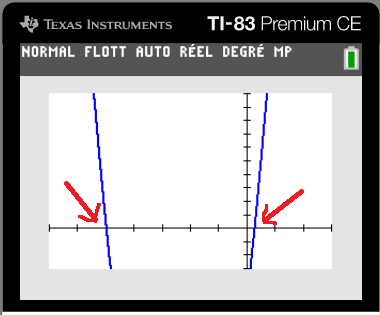
\includegraphics[scale=0.85]{01-03-01}
            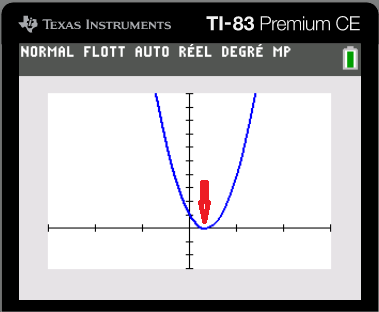
\includegraphics[scale=0.85]{01-03-02}
        \end{multicols}
    \end{brmq}
    
\section{signe d'un trinôme}

    \begin{bintro}
        Pour une fonction polynôme de degré 2 définie par $f(x)=ax^2+bx+c$ :
        \begin{itemRem}
            \item si $a > 0$, sa représentation graphique est une parabole tournée vers le haut.
            \item si $a < 0$, sa représentation graphique est une parabole tournée vers le bas
        \end{itemRem}
    \end{bintro}
    
    \begin{bprop}
        Soit $f$ une fonction polynôme de degré 2 définie sur \R par $f(x)=ax^2+bx+c$:
        \begin{itemProp}
            \item si $\Delta < 0$:\\
            \begin{minipage}[b]{0.5\linewidth}
                \begin{tikzpicture}
                   \tkzTabInit{$x$ / 1 , $f(x)$ / 1}{$-\infty$, $+\infty$}
                   \tkzTabLine{, \text{signe de } a, }
                \end{tikzpicture}
            \end{minipage}
            \begin{minipage}[b]{0.48\linewidth}
                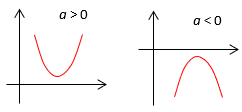
\includegraphics[scale=0.85]{01-03-03}      
            \end{minipage}
            \item si $\Delta = 0$:\\
            \begin{minipage}[b]{0.6\linewidth}
                \begin{tikzpicture}
                   \tkzTabInit{$x$ / 1 , $f(x)$ / 1}{$-\infty$, $x_0$, $+\infty$}
                   \tkzTabLine{, \text{signe de } a, z, \text{signe de } a, }
                \end{tikzpicture}
            \end{minipage}
            \begin{minipage}[b]{0.38\linewidth}
                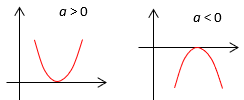
\includegraphics[scale=0.85]{01-03-04}      
            \end{minipage}
            \item si $\Delta > 0$:\\
            \begin{minipage}[b]{0.67\linewidth}
                \begin{tikzpicture}
                   \tkzTabInit[lgt = 1.2, espcl = 2.8, deltacl = 0.5]{$x$ / 1 , $f(x)$ / 1}{$-\infty$, $x_1$,$x_2$, $+\infty$}
                   \tkzTabLine{, \text{signe de } a, z, \text{signe de } -a,z, \text{signe de } a,}
                \end{tikzpicture}
            \end{minipage}
            \begin{minipage}[b]{0.31\linewidth}
                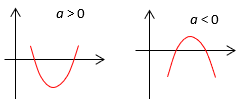
\includegraphics[scale=0.85]{01-03-05}      
            \end{minipage}
        \end{itemProp}
    \end{bprop}
    
    \begin{bmethodet}{Résoudre une inéquation du second degré}
        \grasInMet{Enoncé :} Résoudre l'inéquation : $x^2+3x-5<-x+2$\\
        \ \\
        \grasInMet{Réponse :}\\
            \emph{On commence par rassembler tous les termes dans le membre de gauche afin de pouvoir étudier les signes des trinômes.}\\
            $x^2+3x-5<-x+2$ équivaut à $x^2+4x-7<0$.\\
            Le discriminant de $x^2+4x-7$ est $\Delta = 42 - 4 \times 1 \times (-7) = 44$ et ses racines sont :\\
            $x_1= \dfrac{-4-\sqrt{44}}{2\times1}=-2-\sqrt{11}$ et $x_2= \dfrac{-4+\sqrt{44}}{2\times1}=-2+\sqrt{11}$\\
            On obtient le tableau de signes :\\
            \begin{tikzpicture}
               \tkzTabInit{$x$ / 1 , $f(x)$ / 1}{$-\infty$,$-2-\sqrt{11}$, $-2+\sqrt{11}$, $+\infty$}
               \tkzTabLine{, +, z,- , z, +, }
            \end{tikzpicture}\\
            L'ensemble des solutions de l'inéquation $x^2+3x-5<-x+2$  est donc $\intervOO{-2-\sqrt{11}}{-2+\sqrt{11}}$.
    \end{bmethodet}
    
    \begin{brmq}
        Comme précédement, on peut vérifier le résultat à l'aide de la calculatrice.\\
            \begin{center}
                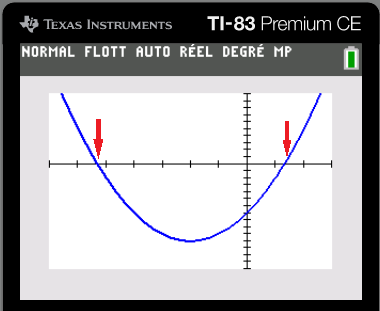
\includegraphics[scale=0.85]{01-03-06}
            \end{center}
    \end{brmq}



\chapter{Vecteurs - partie 1}
\thispagestyle{fancy}

\section{Définitions et propriété}

\subsection{Norme d'un vecteur}

    \begin{bdefi}
        Soit un vecteur $\vv{u}$ et deux points $A$ et $B$ tels que $\vv{u}=\vv{AB}$.\\
        La norme du vecteur $\vv{u}$, notée $\normeB{u}$ est la distance AB.	
    \end{bdefi}
    
\subsection{Produit scalaire}
    \begin{bdefi}
        \begin{minipage}[b]{0.65\linewidth}
            Soit $\vv{u}$ et $\vv{v}$ deux vecteurs du plan.\\
            On appelle \grasInDef{produit scalaire} de $\vv{u}$ par $\vv{v}$, noté $\vv{u}\cdot \vv{v}$, le nombre réel défini par :\\
            \begin{itemDef}
                \item $\vv{u}\cdot \vv{v} =0$, si l'un des deux vecteurs $\vv{u}$ et $\vv{v}$ est nul.
                \item $\vv{u}\cdot \vv{v} =\normeB{u}\times\normeB{v}\times\cos{(\vv{u};\vv{v})}$
            \end{itemDef}
        \end{minipage}\hfill
        \begin{minipage}[b]{0.3\linewidth}
        \begin{center}
            \newrgbcolor{qqwuqq}{0. 0.39215686274509803 0.}
            \psset{xunit=1cm,yunit=1cm,algebraic=true,dimen=middle,dotstyle=o,dotsize=5pt 0,linewidth=1.6pt,arrowsize=3pt 2,arrowinset=0.25}
            \begin{pspicture*}(1.3,0.8)(8.3,4.6)
            \psline[linewidth=1.2pt]{->}(2.,2.)(6.,2.)
            \psline[linewidth=1.2pt]{->}(2.,2.)(4.,4.)
            \rput[tl](3.7,1.8){\Large $\vv u$}
            \rput[tl](2.5,3.6){\Large $\vv v$}
            \pscustom[linewidth=1.2pt,linecolor=qqwuqq]{
\parametricplot{0.0}{0.78}{0.68*cos(t)+2.|0.68*sin(t)+2.}
\lineto(2.,2.)\closepath}
            \begin{scriptsize}
            \psdots[dotsize=5pt 0,dotstyle=*](2.,2.)
            \rput[bl](1.3,2.0){\Large $A$}
            \psdots[dotsize=5pt 0,dotstyle=*](6.,2.)
            \rput[bl](6.2,2.0){\Large $B$}
            \psdots[dotsize=5pt 0,dotstyle=*](4.,4.)
            \rput[bl](4.2,4.0){\Large $C$}
            \end{scriptsize}
            \end{pspicture*}
        \end{center}
        \end{minipage}
    \end{bdefi}
    
    \begin{brmqs}
        \begin{itemRem}
            \item $\vv{u}\cdot \vv{v}$ se lit $\vv{u}$ scalaire $\vv{v}$
            \item 	Si $\vv{AB}$ et $\vv{AC}$ sont deux représentants des vecteurs non nuls $\vv{u}$ et $\vv{v}$ alors :\\
            $\vv{u}\cdot \vv{v} = \vv{AB}\cdot \vv{AC} = \normeB{AB}\times\normeB{AC}\times\cos{(\widehat{BAC})}$
            \item 	\grasInRem{Attention} : Le produit scalaire de deux vecteurs est un nombre réel. Écrire par exemple $\vv{u}\cdot \vv{v}=\vv{0}$ est une maladresse à éviter !
        \end{itemRem}
    \end{brmqs}
    
    \begin{bmethodet}{calculer un produit scalaire}
        \grasInMet{Enoncé :} Calculer : $\vv{AB}\cdot \vv{AC}$ sachant que $AB=5$, $AC=4\sqrt{2}$ et $(\vv{AB},\vv{AC})=\dfrac{\pi}{4}$\\
        \ \\
        \grasInMet{Réponse :}\\
        $\vv{AB}\cdot \vv{AC}= \normeB{AB}\times\normeB{AC}\times\cos{(\vv{AB},\vv{AC})}=5\times 4\sqrt{2} \times \cos{\left(\dfrac{\pi}{4}\right)}=20\sqrt{2}\times\dfrac{\sqrt{2}}{2}=20$
        
    \end{bmethodet}
    
    \begin{bmethodet}{Calculer un produit scalaire à l'aide du cosinus}
        \grasInMet{Enoncé :} \\
        Soit un triangle équilatéral ABC de côté $a$. Calculer, en fonction de a, le produit scalaire $\vv{A B} \cdot \vv{A C}$.
        \begin{center}
            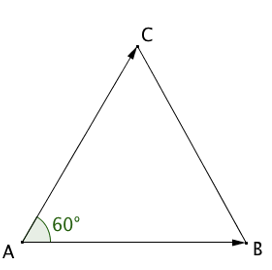
\includegraphics[scale=0.8]{1.04.IMG-01}
        \end{center}

        \ \\
        \grasInMet{Réponse :}\\
        $$
        \begin{array}{l}
        \vv{A B} \cdot \vv{A C}=\|\vv{A B}\| \times\|\vv{A C}\| \times \cos \widehat{B A C} \\
        =a \times a \times \cos 60^{\circ} \\
        =a^{2} \times 0,5 \\
        =\dfrac{a^{2}}{2}
        \end{array}
        $$
        
    \end{bmethodet}
    
    \subsection{Propriété de symétrie du produit scalaire}
    
    \begin{bprop}
        Pour tout vecteur $\vv{u}$ et $\vv{v}$, on a : $\vv{u}\cdot \vv{v}= \vv{v}\cdot \vv{u}$ 
    \end{bprop}
    
    \begin{bdemo}
        On suppose que $\vec{u}$ et $\vec{v}$ sont non nuls (démonstration évidente dans la cas contraire).\\
        $\vec{u} . \vec{v}=\|\vec{u}\| \times\|\vec{v}\| \times \cos (\vec{u} ; \vec{v})$\\
        $=\|\vec{v}\| \times\|\vec{u}\| \times \cos (\vec{u} ; \vec{v})$\\
        $=\|\vec{v}\| \times\|\vec{u}\| \times \cos (-(\vec{v} ; \vec{u}))$\\
        $=\|\vec{v}\| \times\|\vec{u}\| \times \cos (\vec{v} ; \vec{u})$
        $=\vec{v} \cdot \vec{u}$\\
    \end{bdemo}
    
    \subsection{opérations sur les produits scalaires}
    
    \begin{bprop}
        Pour tout vecteur $\vv{u}$,$\vv{v}$ et $\vv{w}$, on a :
        \begin{enumProp}
            \item $\vv{u} \cdot (\vv{v}+\vv{w})=\vv{u} \cdot \vv{v}+\vv{u} \cdot \vv{w}$
            \item $\vv{u} \cdot (k \vv{v})=k \vv{u} \cdot \vv{v}$, avec $k$ un nombre réel.
        \end{enumProp}
    \end{bprop}

    \subsection{Identités remarquables}
    
    \begin{bprop}
        Pour tout vecteur $\vv{u}$ et $\vv{v}$, on a :
        \begin{enumProp}
            \item $\left(\vv{u}+\vv{v}\right)^2=\vv{u}^2 +2\vv{u} \cdot \vv{v}+\vv{v}^2$
            \item $\left(\vv{u}-\vv{v}\right)^2=\vv{u}^2 -2\vv{u} \cdot \vv{v}+\vv{v}^2$
            \item $\left(\vv{u}+\vv{v}\right)\left(\vv{u}-\vv{v}\right)=\vv{u}^2-\vv{v}^2$
        \end{enumProp}
    \end{bprop}
    
    \begin{bdemot}{2ème formule : }
    	
        \begin{align*}
            (\vec{u}-\vec{v})^{2}& =(\vec{u}-\vec{v})(\vec{u}-\vec{v}) \\
            &=\vec{u} \cdot \vec{u}-\vec{u} \cdot \vec{v}-\vec{v} \cdot \vec{u}+\vec{v} \cdot \vec{v} \\
            &=\vec{u}^{2}-2 \vec{u} \cdot \vec{v}+\vec{v}^{2}
        \end{align*}
    \end{bdemot}
    
       \section{Produit scalaire et orthogonalité}
    
    \subsection{Vecteurs orthogonaux}
    
    \begin{bprop}
        Les vecteurs $\vec{u}$ et $\vec{v}$ sont orthogonaux si et seulement si $\vec{u} \cdot \vec{v}=0$.
    \end{bprop}
    
    \begin{bdemo}
        Si l'un des vecteurs est nul, la démonstration est évidente.\\
        Supposons le contraire.\\
        \begin{align*}
            \vec{u} \cdot \vec{v}=0 & \Leftrightarrow\|\vec{u}\| \times\|\vec{v}\| \times \cos (\vec{u} ; \vec{v})=0\\
            &\Leftrightarrow \cos (\vec{u} ; \vec{v})=0\\
            &\Leftrightarrow \text{Les vecteurs\ }\vec{u}\text{\ et\ }  \vec{v}\text{\  sont orthogonaux.}
        \end{align*}
    \end{bdemo}
    
    \subsection{Projection orthogonale}
    
    \begin{bdefi}
        Soit une droite d et un point M du plan.\\
        Le \grasInDef{projeté orthogonal} du point M sur la droite d est le point d'intersection H de la droite d avec la perpendiculaire à d passant par M.
        \begin{center}
            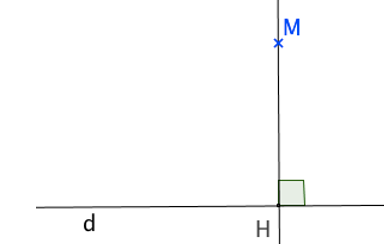
\includegraphics[scale=0.8]{1.04.IMG-04}
        \end{center}
    \end{bdefi}
    
    \begin{bprop}
        Soit $\vec{u}$ et $\vec{v}$ deux vecteurs non nuls du plan tels que $\vec{u}=\vv{O A}$ et $\vec{v}=\vv{O B}$.\\
        H est le projeté orthogonal du point $B$ sur la droite (OA). On a $: \vec{u} . \vec{v}=\vv{O A} \cdot \vv{O B}=\vv{O A} \cdot \vv{O H}$
        \begin{center}
            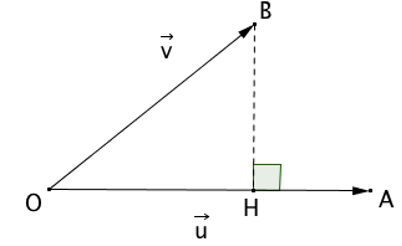
\includegraphics[scale=0.6]{1.04.IMG-06}
        \end{center}
    \end{bprop}
    
    \begin{bdemo}
        $\vv{O A} \cdot \vv{O B}=\vv{O A} \cdot(\vv{O H}+\vv{H B})$\\
$=\vv{O A} \cdot \vv{O H}+\vv{O A} \cdot \vv{H B}$\\
$=\vv{O A} \cdot \vv{O H}$\\
\ \\
En effet, les vecteurs $\vv{O A}$ et $\vv{H B}$ sont orthogonaux donc $\vv{O A} \cdot \vv{H B}=0 .$
    \end{bdemo}
    
    \begin{bmethodet}{Calculer un produit scalaire par projection}
        \grasInMet{Enoncé :}\\
        Soit un carré ABCD de côté $c$. Calculer, en fonction de $c,$ les produits scalaires:
        \begin{center}
            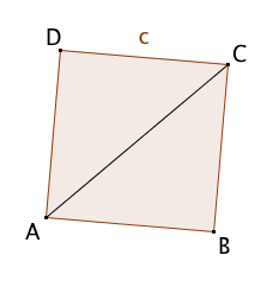
\includegraphics[scale=0.8]{1.04.IMG-07}
        \end{center}
        \begin{multicols}{3}
            \begin{enumMet}
                \item $\vv{A B} \cdot \vv{A C}$
                \item $\vv{A B} \cdot \vv{A D}$
                \item $\vv{A D} \cdot \vv{C B}$
            \end{enumMet}
        \end{multicols}
        
        \grasInMet{Réponse :}\\
        \begin{enumMet}
            \item Par projection, on a :
$\vv{A B} \cdot \vv{A C}=\vv{A B} \cdot \vv{A B}=\|\vv{A B}\|^{2}=c^{2}$
            \item $\vv{A B} \cdot \vv{A D}=0$ car les vecteurs $\vv{A B}$ et $\vv{A D}$ sont orthogonaux.
            \item $\vv{A D} \cdot \vv{C B}=\vv{A D} \cdot \vv{D A}=-\|\vv{A D}\|^{2}=-c^{2}$
        \end{enumMet}
        
    \end{bmethodet}
    
%    \subsection{Transformation de l'expression $\protect\vv{MA}\cdot\protect\vv{MB}$}
%    
%    \begin{propriete}
%        L'ensemble des points $\mathrm{M}$ vérifiant l'égalité $\vv{M A} . \vv{M B}=0$ est le cercle de diamètre [AB].
%    \end{propriete}
%    
%    \begin{demonstration}
%        \begin{center}
%            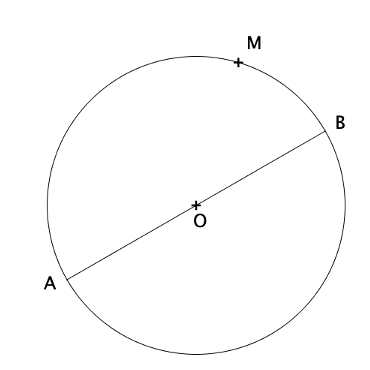
\includegraphics[scale=0.8]{1.04.IMG-08}
%        \end{center}
%        Soit O le milieu du segment [AB]. On a \\
%        $\vv{MA}\cdot \vv{MB}=0$\\
%        $\Leftrightarrow(\vv{M O}+\vv{O A}) \cdot(\vv{M O}+\vv{O B})=0$\\
%        Comme $\mathrm{O}$ est le milieu de $[\mathrm{AB}],$ on $\mathrm{a}: \vv{O B}=-\vv{O A}$ Soit:\\
%        $(M O+\vv{O A}) \cdot(\vv{M O}-\vv{O A})=0$\\
%        $\Leftrightarrow \vv{M O}^{2}-\vv{O A}^{2}=0 \quad \operatorname{car}(\vec{u}+\vec{v}) \cdot(\vec{u}-\vec{v})=\vec{u}^{2}-\vec{v}^{2}$\\
%        $\Leftrightarrow M O^{2}-O A^{2}=0$\\
%        Soit : $M O^{2}=O A^{2}$ soit encore $M O=O A$. M appartient donc au cercle de centre O et de rayon OA, c'est-à-dire le cercle de diamètre [AB].
%    \end{demonstration}
%    
%    \begin{propriete}
%        Un point M, distinct de A et B, appartient au cercle de diamètre [AB] si et seulement si le triangle ABM est rectangle en M.
%    \end{propriete}
%    
%    \begin{remarque}
%        Justification: $\vv{M A} \cdot \vv{M B}=0$ si et seulement si les vecteurs $\vv{M A}$ et $\vv{M B}$ sont orthogonaux.
%        \begin{center}
%            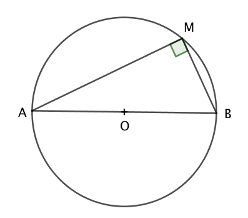
\includegraphics[scale=1]{1.04.IMG-09}
%        \end{center}
%    \end{remarque}
    
    \section{Produit scalaire dans un repère orthonormé}
    
    Le plan est muni d'un repère orthonormé \Rij
    
    \begin{bprop}
        Soit $\vec{u}$ et $\vec{v}$ deux vecteurs de coordonnées respectives $\Coord{u}{x}{y}$ et $\Coord{v}{x'}{y'}$. On a: $\vec{u} \cdot \vec{v}=x x^{\prime}+y y^{\prime}$
    \end{bprop}
    
    \begin{bdemo}
        \begin{align*}
            \vec{u} \cdot \vec{v}&=(x \vec{\imath}+y \vec{\jmath})\left(x^{\prime} \vec{\imath}+y^{\prime} \vec{\jmath}\right)\\
            &=x x^{\prime} \vec{\imath} \cdot \vec{\imath}+x y^{\prime} \vec{\imath} \cdot \vec{\jmath}+y x^{\prime} \vec{\jmath} \cdot \vec{\imath}+y y^{\prime} \vec{\jmath} \cdot \vec{\jmath}\\
            &=x x^{\prime}\|\vec{\imath}\|^{2}+x y^{\prime} \vec{\imath} \cdot \vec{\jmath}+y x^{\prime} \vec{\jmath} \cdot \vec{\imath}+y y^{\prime}\|\vec{j}\|^{2}\\
            &=x x^{\prime}+y y^{\prime}
        \end{align*}
        car $\|\vec{\imath}\|=\|\vec{j}\|=1$, le repère étant normé, et $\vec{\imath} \cdot \vec{\jmath}=\vec{\jmath} \cdot \vec{\imath}=0$, le repère étant orthogonal.
    \end{bdemo}
    
    \begin{bmethodet}{Calculer un produit scalaire à l'aide des coordonnées}
        \grasInMet{Enoncé :}\\
        Soit $\Coord{u}{5}{-4}$ et $\Coord{v}{-3}{7}$ deux vecteurs.\\
        Calculer $\vec{u} \cdot \vec{v}$
        \ \\
        \grasInMet{Réponse :}\\
        $\vec{u} \cdot \vec{v}=5 \times(-3)+(-4) \times 7=-15-28=-43$
    \end{bmethodet}


    \begin{bmethodet}{Déterminer un angle à l'aide du produit scalaire}
        \grasInMet{Enoncé :}\\
        Calculer la mesure de l'angle $(\vv{A B} ; \vv{C D})$ en lisant les coordonnées des points $\mathrm{A}, \mathrm{B}, \mathrm{C}$ et $\mathrm{D}$ dans le repère.\\
        \begin{center}
            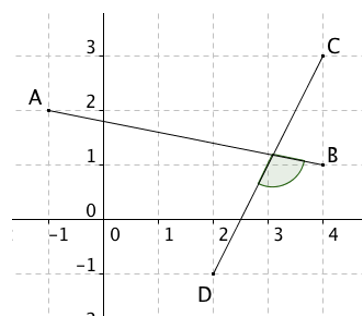
\includegraphics[scale=0.8]{1.04.IMG-10}
        \end{center}
        \ \\
        \grasInMet{Réponse :}\\
        On a :\\
    $\vv{A B} \cdot \vv{C D}=\|\vv{A B}\| \times\|\vv{C D}\| \times \cos (\vv{A B} ; \vv{C D})$\\
    $=\sqrt{(4-(-1))^{2}+(2-1)^{2}} \times \sqrt{(4-2)^{2}+(3-(-1))^{2}} \times \cos (\vv{A B} ; \vv{C D})$\\
    $=\sqrt{520} \times \cos (\vv{A B} ; \vv{C D})$\\
    $=2 \sqrt{130} \times \cos (\vv{A B} ; \vv{C D})$\\
    \ \\
    On a également $: \vv{A B}(5 ;-1)$ et $\vv{C D}(-2 ;-4),$ donc $\vv{A B} \cdot \vv{C D}=5 \times(-2)+(-1) \times(-4)=-6$\\
    On a ainsi $: 2 \sqrt{130} \times \cos (\vv{A B} ; \vv{C D})=-6$\\
    Et donc $: \cos (\vv{A B} ; \vv{C D})=-\frac{6}{2 \sqrt{130}}=-\frac{3}{\sqrt{130}}$\\
    Et $:(\vv{A B} ; \vv{C D}) \approx 105,3^{\circ}$\\
    \end{bmethodet}
    
    % \section{Produit scalaire et norme}
    
    % \subsection{Propriétés}

    % Soit un vecteur $\vec{u},$ on a :
    % $\vec{u} \cdot \vec{u}=\|\vec{u}\| \times\|\vec{u}\| \times \cos (\vec{u} ; \vec{u})=\|\vec{u}\|^{2} \times \cos 0=\|\vec{u}\|^{2}$\\
    % et\\
    % $\vec{u}\cdot \vec{u}=\vec{u}^{2}$\\
    % On a ainsi $: \vec{u}^{2}=\vec{u} \cdot \vec{u}=\|\vec{u}\|^{2}$
    
    % \begin{propriete}
    %     Propriété : Soit $\vec{u}$ et $\vec{v}$ deux vecteurs. On a :
    %     \begin{itemDef}
    %         \item $\vec{u} \cdot \vec{v}=\dfrac{1}{2}\left(\|\vec{u}\|^{2}+\|\vec{u}\|^{2}-\|\vec{u}-\vec{v}\|^{2}\right)$
    %         \item $\vec{u} \cdot \vec{v}=\dfrac{1}{2}\left(\|\vec{u}+\vec{v}\|^{2}-\|\vec{u}\|^{2}-\|\vec{v}\|^{2}\right)$
    %         \item $\vec{u} \cdot \vec{v}=\dfrac{1}{4}\left(\|\vec{u}+\vec{v}\|^{2}-\|\vec{u}-\vec{v}\|^{2}\right)$
    %     \end{itemDef}
    % \end{propriete}
    
    % \begin{demonstrationTitre}{Démonstration de la première formule}
    %     \begin{align*}
    %         \|\vec{u}-\vec{v}\|^{2}&=(\vec{u}-\vec{v})^{2} \\
    %         &=\vec{u}^{2}-2 \vec{u} \cdot \vec{v}+\vec{v}^{2} \\
    %         &=\|\vec{u}\|^{2}-2 \vec{u} \cdot \vec{v}+\|\vec{v}\|^{2}
    %     \end{align*}
    %     Donc $\vec{u} \cdot \vec{v}=\dfrac{1}{2}\left(\|\vec{u}\|^{2}+\|\vec{u}\|^{2}-\|\vec{u}-\vec{v}\|^{2}\right)$
    % \end{demonstrationTitre}

    % \begin{propriete}
    %     Soit $A, B$ et $C$ trois points du plan. On a :
    %     $\vv{A B} \cdot \vv{A C}=\dfrac{1}{2}\left(A B^{2}+A C^{2}-B C^{2}\right)$
    % \end{propriete}
    
    % \begin{demonstration}
    %     \begin{align*}
    %         \vv{A B} \cdot \vv{A C}&=\dfrac{1}{2}\left(\|\vv{A B}\|^{2}+\|\vv{A C}\|^{2}-\|\vv{A B}-\vv{A C}\|^{2}\right) \\
    %         &=\dfrac{1}{2}\left(A B^{2}+A C^{2}-\|\vv{C B}\|^{2}\right) \\
    %         &=\dfrac{1}{2}\left(A B^{2}+A C^{2}-B C^{2}\right)
    %     \end{align*}
    % \end{demonstration}
    
    % \begin{exemple}
    %     Si $\mathrm{AB}=6, \mathrm{AC}=5$ et $\mathrm{CB}=4$ alors:
    %     $$
    %     \vv{A B} \cdot \vv{A C}=\frac{1}{2}\left(A B^{2}+A C^{2}-C B^{2}\right)=\frac{1}{2}\left(6^{2}+5^{2}-4^{2}\right)=\frac{1}{2}(36+25-16)=\frac{45}{2}
    %     $$
    % \end{exemple}
    
    % \begin{methodeTitre}{Calculer un produit scalaire à l'aide des normes}
    %     \grasInMet{Enoncé :}\\
    %     On considère la figure ci-dessous, calculer le produit scalaire $\vv{C G} \cdot \vv{C F}$
    %     \begin{center}
    %         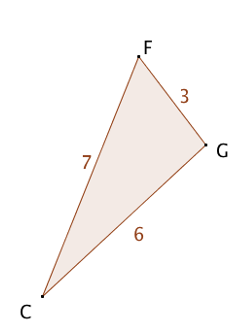
\includegraphics[scale=0.8]{1.04.IMG-02}
    %     \end{center}
    %     \ \\
    %     \grasInMet{Réponse :}\\
    %     $\vv{C G} \cdot \vv{C F}=\frac{1}{2}\left(C G^{2}+C F^{2}-G F^{2}\right)$\\
    %     $=\dfrac{1}{2}\left(6^{2}+7^{2}-3^{2}\right)$\\
    %     $=38$
    % \end{methodeTitre}
    
    % \subsection{Théorème d'Al Kashi}
    
    % \begin{theoreme}
    %     Dans un triangle $\mathrm{ABC},$ on a, avec les notations de la figure :
    %     $$
    %     a^{2}=b^{2}+c^{2}-2 b c \cos \hat{A}
    %     $$
    %     \begin{center}
    %         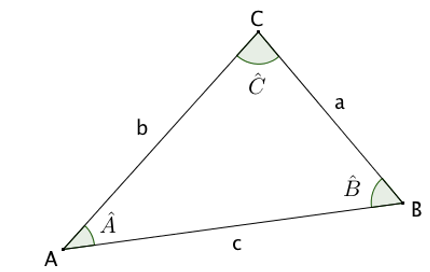
\includegraphics[scale=0.8]{1.04.IMG-03}
    %     \end{center}
    % \end{theoreme}
    
    % \begin{demonstration}
    %     $\vv{A B} \cdot \vv{A C}=A B \times A C \times \cos \hat{A}=b c \cos \hat{A}$\\
    %     et\\
    %     $\vv{A B} \cdot \vv{A C}=\frac{1}{2}\left(A B^{2}+A C^{2}-B C^{2}\right)=\frac{1}{2}\left(b^{2}+c^{2}-a^{2}\right)$\\
    %     Donc $: \frac{1}{2}\left(b^{2}+c^{2}-a^{2}\right)=b c \cos \hat{A}$\\
    %     Soit $: b^{2}+c^{2}-a^{2}=2 b c \cos \hat{A}$\\
    %     Soit encore $: a^{2}=b^{2}+c^{2}-2 b c \cos \hat{A}$\\
    % \end{demonstration}
    
    % \begin{methodeTitre}{Calculer un produit scalaire à l'aide des normes}
    %     \grasInMet{Enoncé :}\\
    %     On considère la figure ci-dessous, calculer la mesure de l'angle $\widehat{B A C}$ au degré près.
    %     \begin{center}
    %         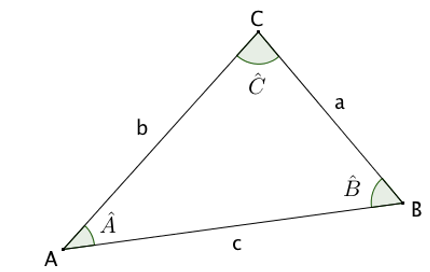
\includegraphics[scale=0.8]{1.04.IMG-03}
    %     \end{center}
    %     \ \\
    %     \grasInMet{Réponse :}\\
    %     D'après le théorème d'Al Kashi, on a :\\
    %     $C B^{2}=A B^{2}+A C^{2}-2 \times A B \times A C \times \cos \widehat{B A C}$\\
    %     $4^{2}=6^{2}+5^{2}-2 \times 6 \times 5 \times \cos \widehat{B A C}$\\
    %     $16=36+25-60 \cos \widehat{B A C}$\\
    %     $60 \cos \widehat{B A C}=36+25-16$\\
    %     $60 \cos \widehat{B A C}=45$\\
    %     $\cos \widehat{B A C}=\dfrac{45}{60}$\\
    %     $\cos \widehat{B A C}=\dfrac{3}{4}$\\
    %     $\widehat{B A C} \approx 41^{\circ}$
    % \end{methodeTitre}
    
    % \section{Vecteur Normal}
    
    % \subsection{définition et propriétés}
    
    % \begin{definition}
    %     Un \grasInDef{vecteur normal} à une droite $d$ quelconque du plan est un vecteur non nul et orthogonal à un vecteur directeur de $d$.
    % \end{definition}
    
    % \begin{propriete}
    %     Deux droites du plan sont perpendiculaires si et seulement si un vecteur normal de l'une est orthogonal à un vecteur normal de l'autre.
    % \end{propriete}
    
    % \begin{demonstration}
    %     On suppose que $d$ et $d^{\prime}$ sont perpendiculaires. Si $\vec{u}$ est un vecteur directeur de $d$ et $\vec{v}$ de $d^{\prime},$ alors $\vec{u}$ et $\vec{v}$ sont orthogonaux. $\vec{v}$ étant normal à $d$ et $\vec{u}$ à $d^{\prime},$ la propriété est vérifiée.\\
    %     Réciproquement, si $\vec{u},$ vecteur normal à $d,$ est orthogonal à $\vec{v},$ vecteur normal à $d^{\prime},$ alors $\vec{v}$ est un vecteur directeur de $d$ et $\vec{u}$ de $d^{\prime} .$ Ayant des vecteurs directeurs orthogonaux, d et $d^{\prime}$ sont perpendiculaires.
    % \end{demonstration}
    
    % \begin{methode}
    %     \grasInMet{Enoncé:}\\
    %     Soit $d$ une droite de vecteur directeur $\Coord{u}{3}{5}$.
    %     \begin{enumMet}
    %         \item Déterminer une condition sur les coordonnées d'un vecteur $\vv{n}$ non nul pour qu'il soit normal à $d$.
    %         \item Le vecteur $\Coord{v}{-10}{6}$ est-il un vecteur normal à $d$?
    %     \end{enumMet}
        
    %     \grasInMet{Réponse:}\\
    %     \begin{enumMet}
    %         \item Si $\Coord{n}{x}{y}$ est un vecteur normal à $d$, alors il est orthogonal à $\vv{u}$.\\
    %         Donc $\vv{u} \cdot \vv{n}=3 x+5 y=0$ soit $y=-\dfrac{3}{5} x$.\\
    %         Les coordonnées de $\vv{n}$ sont donc de la forme $\CoordSV{x}{-\dfrac{3}{5}x}$ avec $x \in \R$.
    %         \item On calcule le produit scalaire $\vv{u}\cdot\vv{v}$\\
    %         $\vv{u}\cdot\vv{v}=3\times(-10)+5\times6=-30+30=0$\\
    %         le vecteur $\vv{v}$ est orthogonal au vecteur directeur $\vv{u}$ de la droite $d$, donc $\vv{v}$ est un vecteur normal à $d$. 
    %     \end{enumMet}
    % \end{methode}
    
    % \subsection{Équations cartésiennes et vecteur normal}
    
    % \begin{proprieteTitre}{Rappel : équations cartésiennes}
    %     Toute droite $D$ admet une équation de la forme $a x+b y+c=0$ avec $(a ; b) \neq(0 ; 0) .$ Un \grasInDef{vecteur directeur} de $D$ est $\Coord{u}{-b}{a}$ \\
    %     Cette équation est appelée \grasInDef{équation cartésienne} de la droite $D$.
    % \end{proprieteTitre}
        
    % \begin{propriete}
    %     Soient $a, b$ et $c$ trois réels tels que $a$ et $b$ ne sont pas simultanément nuls.\\
    %     La droite d'équation cartésienne $a x+b y+c=0$ admet pour \grasInDef{vecteur normal} le vecteur $\Coord{n}{a}{b}$.\\
    %     \ \\
    %     Réciproquement, toute droite ayant pour \grasInDef{vecteur normal} le vecteur non nul $\Coord{n}{a}{b}$ admet une équation cartésienne de la forme $a x+b y+c=0$.
    % \end{propriete}
        
    % \begin{exemple}
    %     La droite d'équation cartésienne $3 x-4 y+5=0$ admet pour vecteur normal le vecteur $\Coord{n}{3}{-4}$  et pour vecteur directeur le vecteur $\Coord{u}{4}{3}$.\\
    %     On a bien $\vv{n} \cdot \vv{u}=0$
    % \end{exemple}
    
    % \begin{methode}
    %     \grasInMet{Enoncé:}\\
    %     Dans un repère orthonormé, déterminer, de deux façons différentes, une équation cartésienne de la droite $d$ passant par le point $\mathrm{A}(5 ;-1)$ et de vecteur normal $\Coord{n}{2}{-3}$.
        
    %     \grasInMet{Réponse:}\\
    %     \begin{enumMet}
    %         \item 1. On lit sur le vecteur normal que $a=2$ et $b=-3$.
    %         Donc une équation de $d$ est de la forme $2 x-3 y+c=0$. $\mathrm{A}(5 ;-1) \in d$ donc $2 \times 5-3 \times(-1)+c=0$ et donc $c=-13$.\\
    %         Ainsi, une équation de la droite $d$ est $2 x-3 y-13=0$.
    %         \item Soit $\mathrm{M}(x ;y)$ appartenant à $d .$ Alors $\vv{\mathrm{AM}}$ est un vecteur directeur de $d$ et est orthogonal au vecteur $\vv{n}$.\\
    %         $\vv{\mathrm{AM}} \cdot \vv{n}=0 \iff \CoordSV{x-5}{y+1} \cdot \CoordSV{2}{-3}=0 \iff 2(x-5)-3(y+1)=0 \iff 2 x-3 y-13=0$\\
    %         Donc une équation de la droite $d$ est $2 x-3 y-13=0$
    %     \end{enumMet}
    % \end{methode}


\graphicspath{{./1.05 - Fonction sinus et cosinus/images/}}
\chapter{Fonction sinus et cosinus}
\thispagestyle{fancy}

\vspace{-0.5cm}

	\section{Résoudre une équation trigonométrique}
	
		\begin{bmethodet}{Résoudre une équation trigonométrique}
			\grasInMet{Enoncé :}\\
			Résoudre sur $[3\pi;5\pi]$ l'équation $\cos x=\dfrac{\sqrt{3}}{2}$
			\grasInMet{Réponse :}\\
			\ \\
			\begin{minipage}{0.65\linewidth}
				On commence par étudier la solution dans l'intervalle\\ $]-\pi;\pi]$ (parmi les mesures principales de l'angle).\\
				L'équation $\cos x=\dfrac{\sqrt{3}}{2}$ a pour solution :\\
				$\begin{cases}
					x_1 &=\dfrac{\pi}{6}\\
					x_2 &=-\dfrac{\pi}{6}
					\end{cases}$\\
				On en déduit les solutions sur \R.\\
				L'équation $\cos x=\dfrac{\sqrt{3}}{2}$ a pour solution ($k\in \Z$ ) :\\
				$\begin{cases}
						x_1 &=\dfrac{\pi}{6}+2k\pi\\
						x_2 &=-\dfrac{\pi}{6}+2k\pi\
					\end{cases}$\\
				On teste différentes valeurs de $k$ pour trouver les valeurs qui appartiennent à l'intervalle souhaité $[3\pi;5\pi]$ (ou $\left[\dfrac{18\pi}{12};\dfrac{30\pi}{6}\right]$)\\
				$k=1\quad \begin{cases}
						x_1 &=\dfrac{\pi}{6}+2\pi=\dfrac{13\pi}{6}\notin\left[\dfrac{18\pi}{12};\dfrac{30\pi}{6}\right]\\
						x_2 &=-\dfrac{\pi}{6}+2\pi=\dfrac{11\pi}{6}\notin\left[\dfrac{18\pi}{12};\dfrac{30\pi}{6}\right]
					\end{cases}$\\
				$k=2\quad \begin{cases}
						x_1 &=\dfrac{\pi}{6}+4\pi=\dfrac{25\pi}{6}\in\left[\dfrac{18\pi}{12};\dfrac{30\pi}{6}\right]\\
						x_2 &=-\dfrac{\pi}{6}+4\pi=\dfrac{23\pi}{6}\in\left[\dfrac{18\pi}{12};\dfrac{30\pi}{6}\right]
					\end{cases}$\\
				$k=3\quad \begin{cases}
						x_1 &=\dfrac{\pi}{6}+6\pi=\dfrac{37\pi}{6}\notin\left[\dfrac{18\pi}{12};\dfrac{30\pi}{6}\right]\\
						x_2 &=-\dfrac{\pi}{6}+6\pi=\dfrac{35\pi}{6}\notin\left[\dfrac{18\pi}{12};\dfrac{30\pi}{6}\right]
					\end{cases}$\\
				On peut maintenant conclure : $S=\left\{\dfrac{23\pi}{6};\dfrac{25\pi}{6}\right\}$
				\end{minipage} \hfill
				\begin{minipage}{0.35\linewidth}
					\begin{center}
							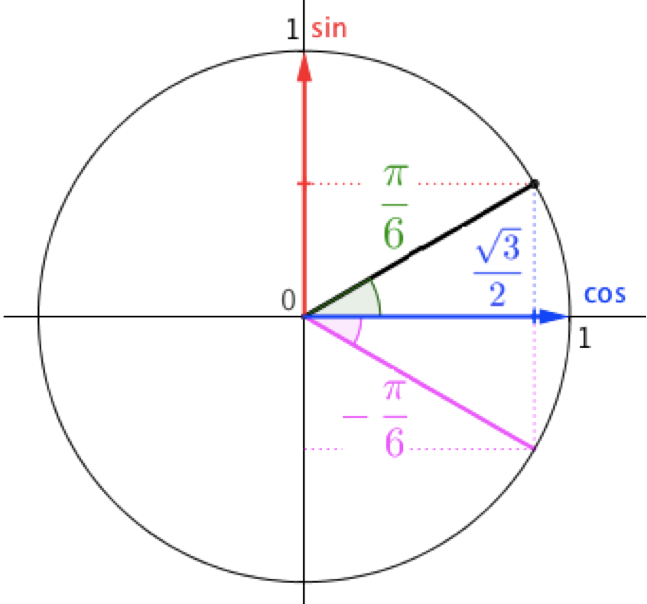
\includegraphics[scale=0.35]{01-02-16}
						\end{center}
				\end{minipage}
				
			\end{bmethodet}

%     \section{Représentations graphiques}
%     \begin{center}
%         \includegraphics[scale=0.4]{../images/01-02-18.png}\\
%         Fonction cosinus
%     \end{center}
%     \begin{center}
%         \includegraphics[scale=0.4]{../images/01-02-19.png}\\
%         Fonction sinus
%     \end{center}
%    
%     \section{Périodicité}
%    
%     On a vu que :  $\cos x=\cos(x+2k\pi)$ où $k$ entier relatif et  $\sin x=\sin(x+2k\pi)$ où $k$ entier relatif.
%    
%     \begin{bprop}
%         On dit que les fonctions cosinus et sinus sont \grasInDef{périodiques de période $2\pi$}.
%     \end{bprop}
%    
%     \begin{bcscq}
%         Pour tracer la courbe représentative de la fonction cosinus ou de la fonction sinus, il suffit de la tracer sur un intervalle de longueur $2\pi$ et de la compléter par translation.
%     \end{bcscq}
%    
%     \section{Parité}
%    
%     On a vu que :  $\cos(-x)=\cos(x)$ et  $\sin(-x)=-\sin x$.
%    
%     \begin{bprop}
%         On dit que la fonctions \grasInDef{cosinus est paire} et que la fonction \grasInDef{sinus est impaire}.
%     \end{bprop}
%    
%     \begin{bcscq}
%         - Dans un repère orthogonal, la courbe représentative de la fonction cosinus est symétrique par rapport à l'axe des ordonnées.\\
%         - Dans un repère orthogonal, la courbe représentative de la fonction sinus est symétrique par rapport à l'origine.
%     \end{bcscq}
%    
%     \section{Variations des fonctions cosinus et sinus}
%    
%         \begin{multicols}{2}
%             \begin{tikzpicture}
%                 \tkzTabInit{$x$ / 1 , $\sin(x)$ / 1.5}{$0$, $\dfrac{\pi}{2}$, $\pi$}
%                 \tkzTabVar{-/ 0, +/ 1, -/ 0}
%             \end{tikzpicture}
%            
%             \begin{tikzpicture}
%                 \tkzTabInit{$x$ /1, $\cos(x)$ /1.5} {$0$ , $\pi$}
%                 \tkzTabVar{+/ 1, -/ -1}
%             \end{tikzpicture}
%         \end{multicols}
     
%     \section{Fonctions cosinus et sinus}
     
     \section{Définitions et représentations graphiques}
     \begin{bdefis}
     	\begin{itemDef}
     		\item La fonction cosinus est la fonction définie sur $\mathbb{R}$ qui, à tout réel $x$, associe $\cos (x)$.
     		\item La fonction sinus, est la fonction définie sur $\mathbb{R}$ qui, à tout réel $x$, associe $\sin (x)$.
     	\end{itemDef}
     
     	
     \end{bdefis}
 
 	\begin{minipage}[c]{0.45\linewidth}
 		\begin{center}
 			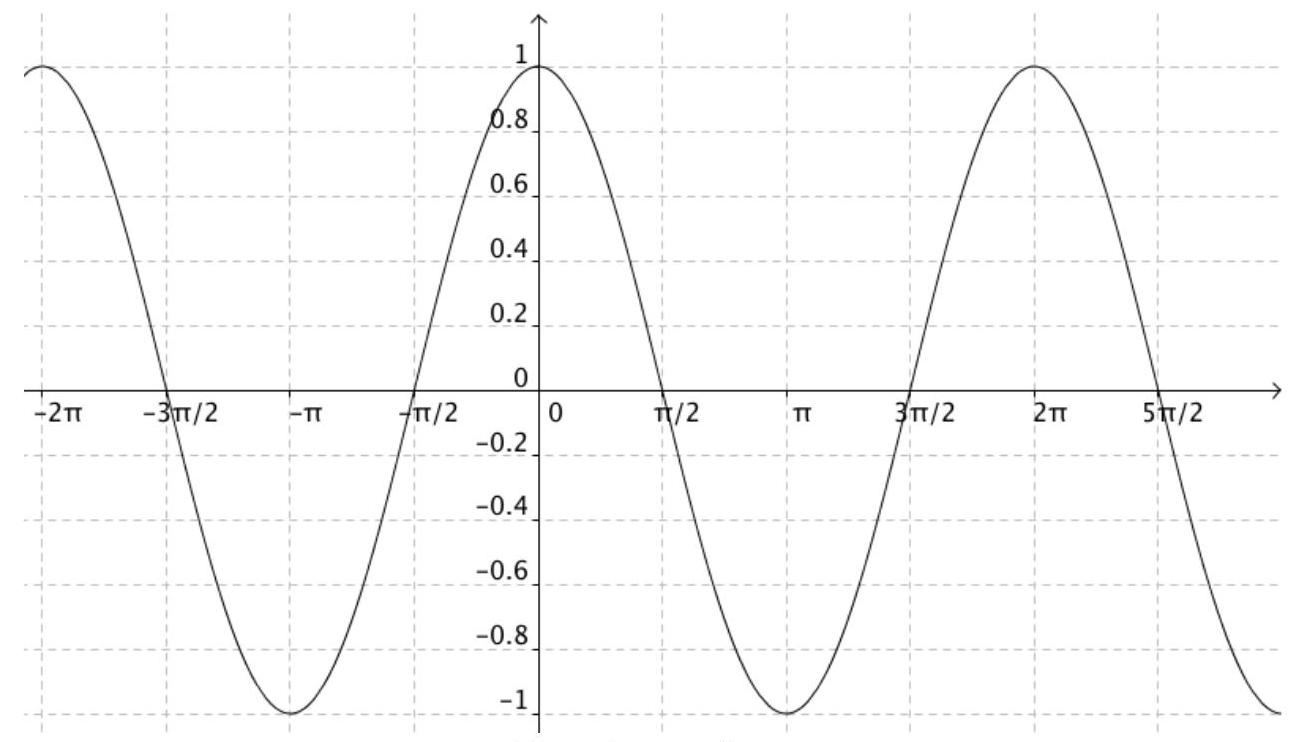
\includegraphics[scale=0.15]{2024_01_04_295cf56f03985ebac5b3g-06(1)}
 		\end{center}
 		
 		Fonction cosinus
 	\end{minipage} \hfill
 	\begin{minipage}[c]{0.45\linewidth}
 		\begin{center}
 			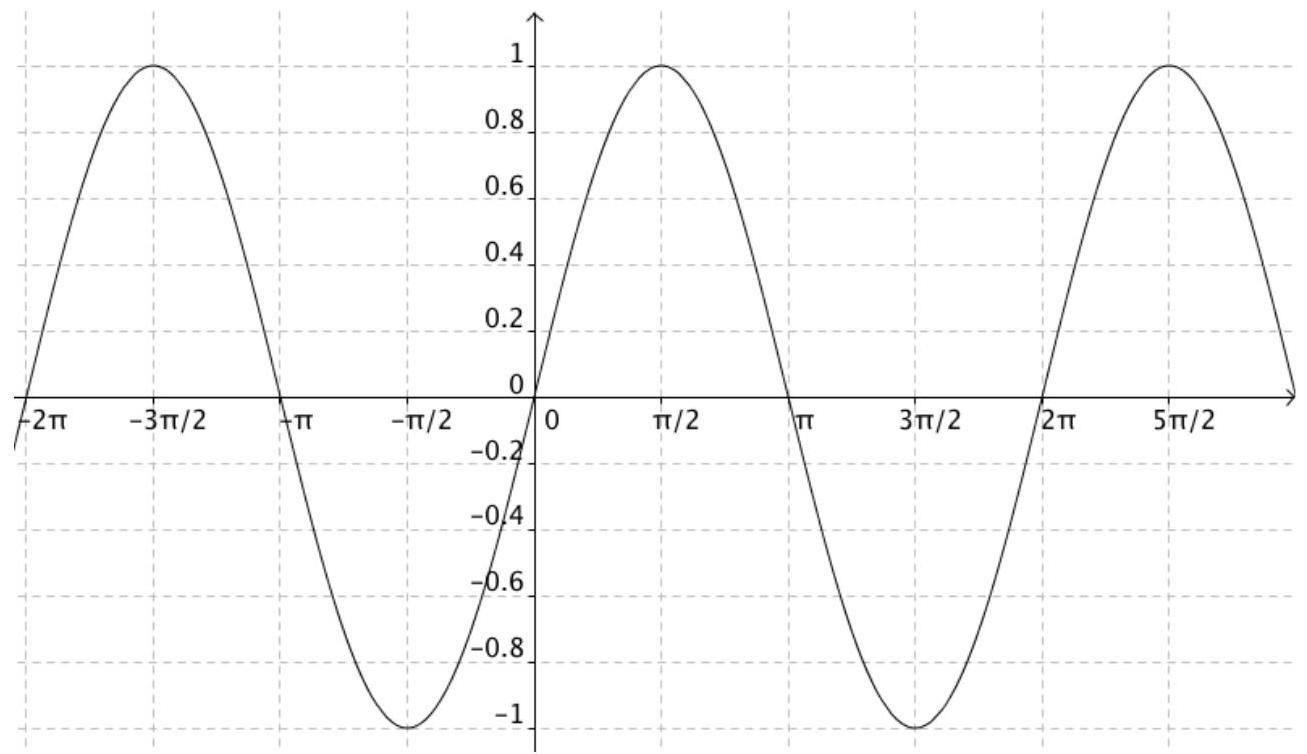
\includegraphics[scale=0.15]{2024_01_04_295cf56f03985ebac5b3g-06}
 		\end{center}
 		
 		Fonction sinus
 	\end{minipage}
     
     
     
     
     
     \section{Périodicité}
     
     \begin{bprops}
     	\begin{itemProp}
     		\item $\cos (x)=\cos (x+2 k \pi)$ où $k$ entier relatif.
     		\item $\sin (x)=\sin (x+2 k \pi)$ où $k$ entier relatif.
     	\end{itemProp}
     \end{bprops}
     
     \begin{bdemo}
     	Aux points de la droite orientée d'abscisses $x$ et $x+2 k \pi$ ont fait correspondre le même point du cercle trigonométrique.
     \end{bdemo}
 
 	\begin{brmq}
 		On dit que les fonctions cosinus et sinus sont périodiques de période $2 \pi$.
 		
 		Cela signifie qu'on retrouve le même morceau de courbe sur chaque intervalle de longueur $2 \pi$.
 	\end{brmq}
     
     \subsection{Fonction cosinus}
     \begin{center}
     	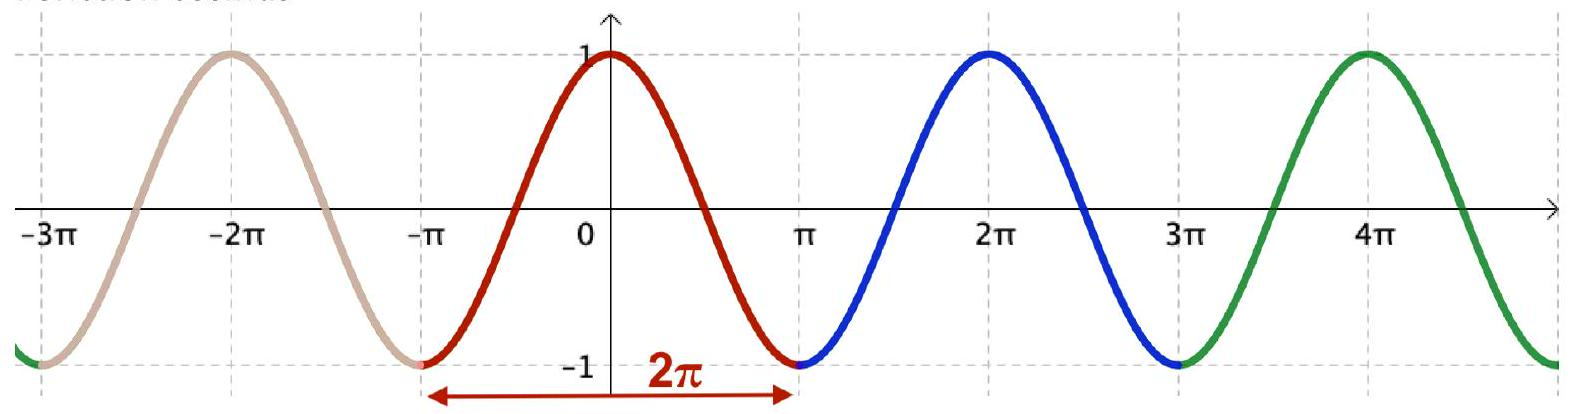
\includegraphics[scale=0.2]{2024_01_04_295cf56f03985ebac5b3g-07(2)}
     \end{center}
     
    
     \subsection{ Fonction sinus}
     \begin{center}
     	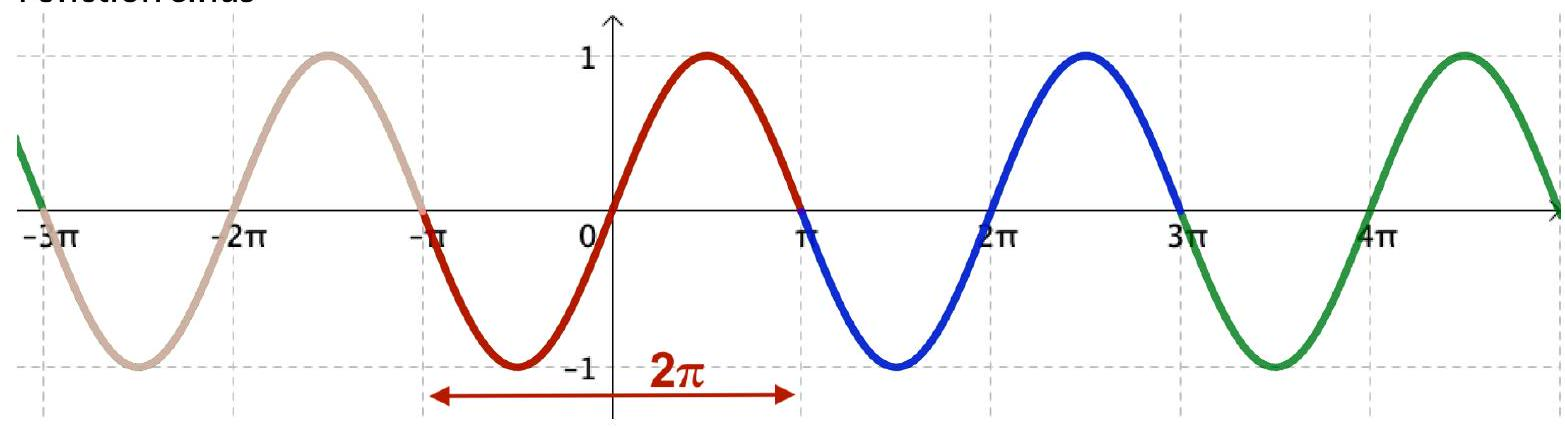
\includegraphics[scale=0.2]{2024_01_04_295cf56f03985ebac5b3g-07(1)}
     \end{center}
 
 	\section{Parité}
     
     \begin{bdefis}
     	\begin{itemDef}
     		\item Une fonction dont la courbe est symétrique par rapport à l'axe des ordonnées est une fonction paire.
     		\item Une fonction dont la courbe est symétrique par rapport à l'origine du repère est une fonction impaire.
     	\end{itemDef}	
     \end{bdefis}
     	
     
    \begin{brmqs}
    	\begin{itemRem}
    		\item Pour une fonction paire, on a : $f(-x)=f(x)$.
    		\item Pour une fonction impaire, on a : $f(-x)=-f(x)$.
    	\end{itemRem}
    	Ce sont ces résultats qu'il faudra vérifier pour prouver qu'une fonction est paire ou impaire.	
    \end{brmqs}
    
     
     
     \begin{bprops}
     	\begin{itemProp}
     		\item La fonction cosinus est paire et on a : $\cos (-x)=\cos (x)$
     		\item La fonction sinus est impaire et on a : $\sin (-x)=-\sin (x)$
     	\end{itemProp}	
     \end{bprops}
     
     \begin{bdemo}
     	Les angles de mesures $x$ et $-x$ sont symétriques par rapport à l'axe des abscisses donc :
     	
     	$\sin (-x)=-\sin x$ et $\cos (-x)=\cos x$.
     	
     	\begin{center}
     		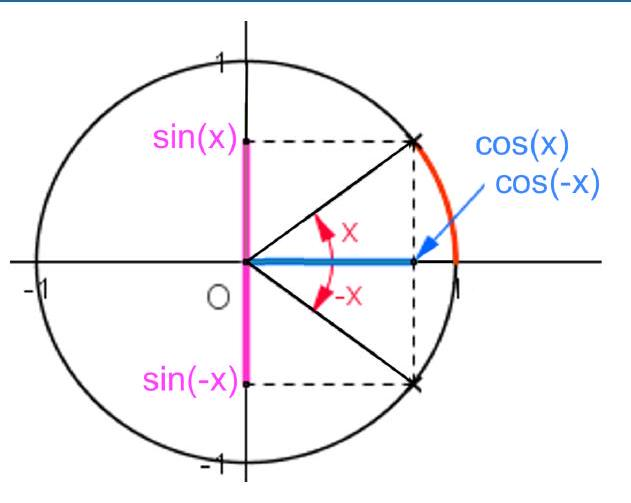
\includegraphics[scale=0.2]{2024_01_04_295cf56f03985ebac5b3g-07}
     	\end{center}
     \end{bdemo}
     
     \begin{brmqs}
     	\begin{itemRem}
     		\item La courbe de la fonction cosinus est symétrique par rapport à l'axe des ordonnées.
     		\item La courbe de la fonction sinus est symétrique par rapport à l'origine.
     	\end{itemRem}
     \end{brmqs}
 
 	\section{Méthodes}
     
     \begin{bmethodet}{Reconnaître graphiquement la parité et la périodicité d'une fonction}
     	\grasInMet{Enoncé:}\\
     	Déterminer graphiquement la parité et la périodicité des fonctions $f, g$ et $h$ représentées ci-dessous :
     	\begin{center}
     		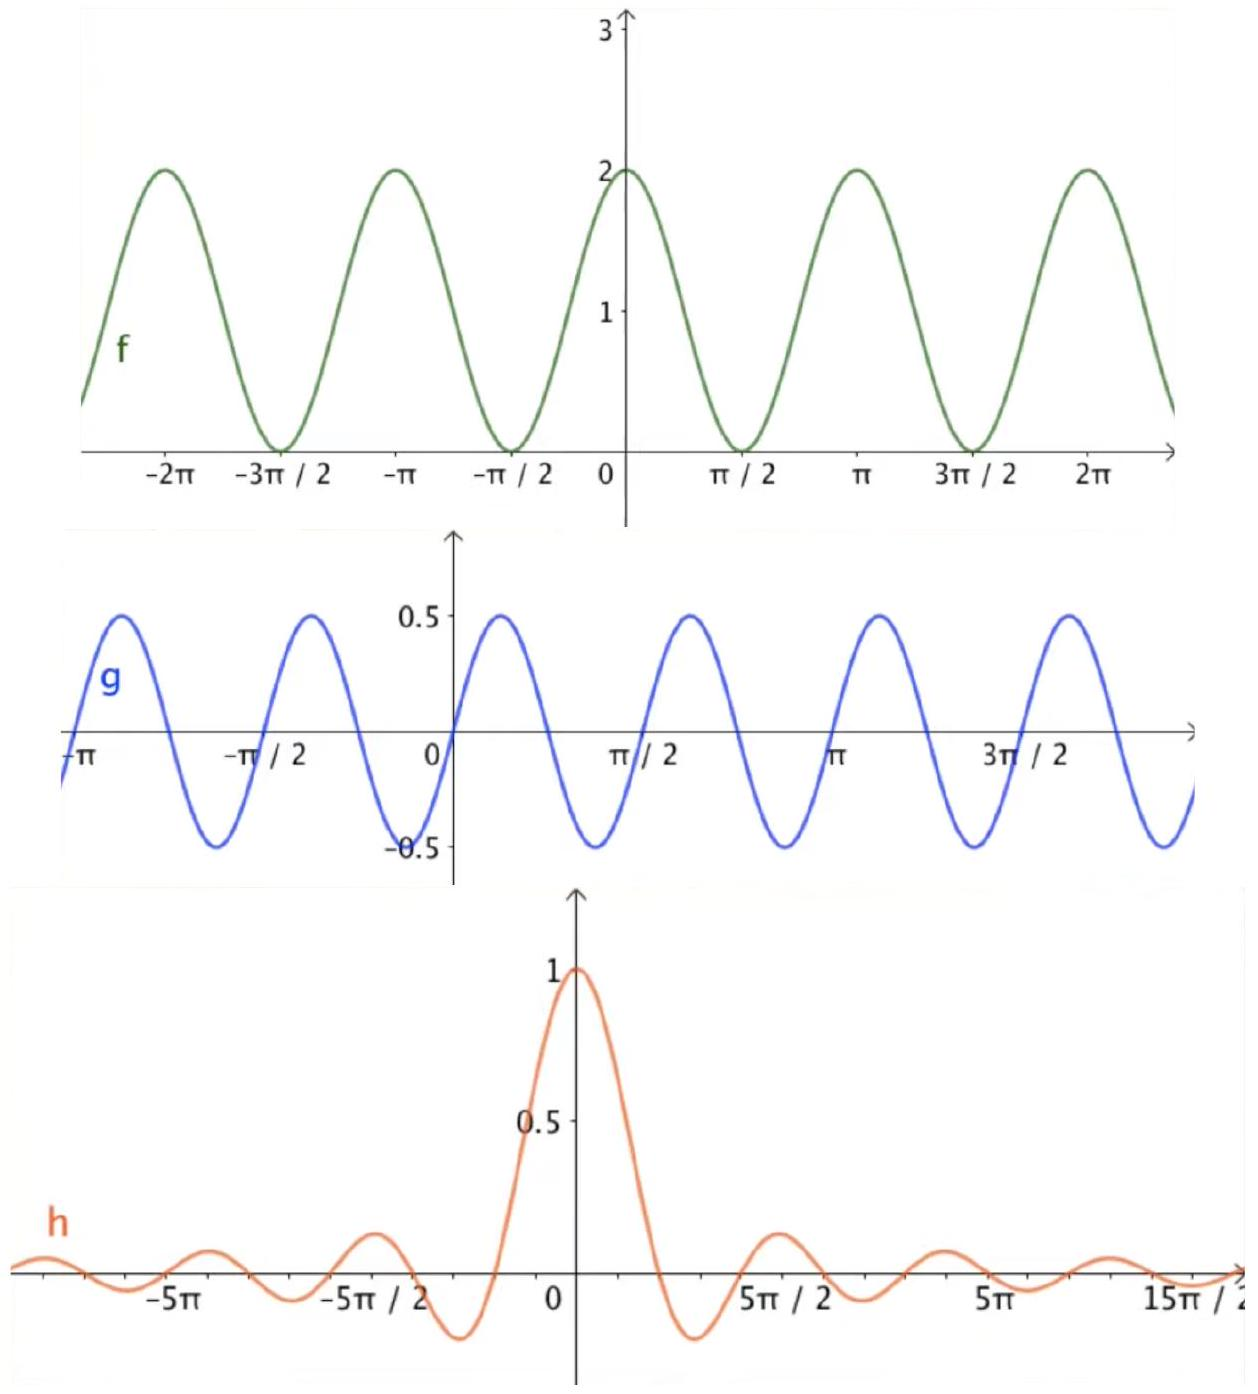
\includegraphics[scale=0.2]{2024_01_04_295cf56f03985ebac5b3g-08}
     	\end{center}
     	\grasInMet{Corrigé:}\\
     	\grasInMet{- FONCTION $\boldsymbol{f}$ :}\\
     	La fonction $f$ est paire car sa courbe est symétrique par rapport à l'axe des ordonnées.
     	\begin{center}
     		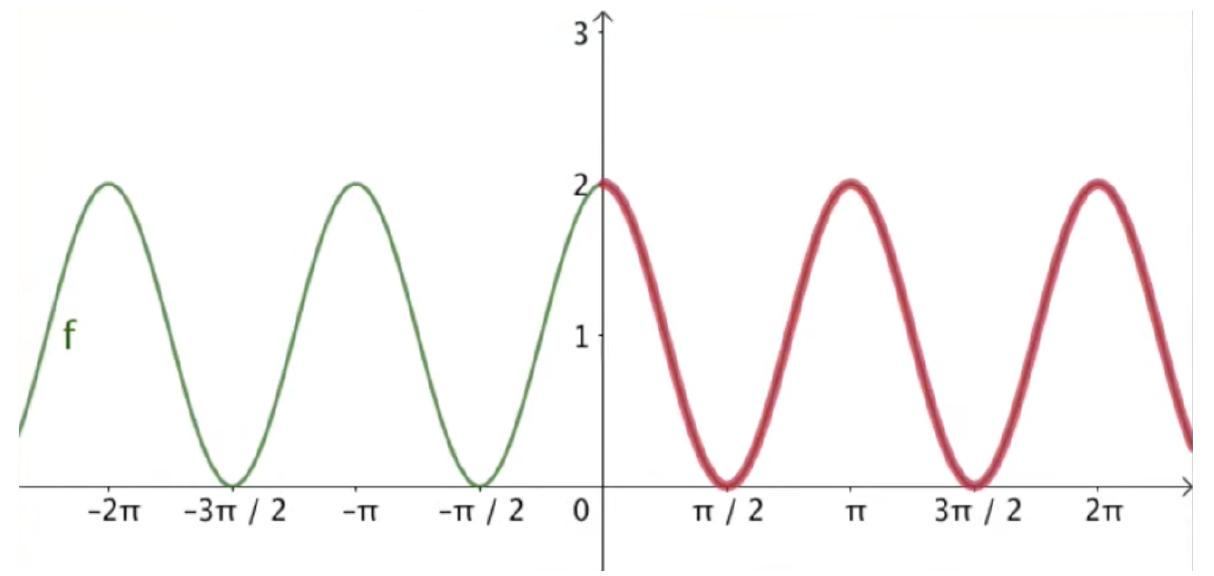
\includegraphics[scale=0.15]{2024_01_04_295cf56f03985ebac5b3g-09(2)}
     	\end{center}
     	La fonction $f$ est périodique de période $\pi$ car on retrouve le même morceau de courbe sur chaque intervalle de longueur $\pi$.
     	\begin{center}
     		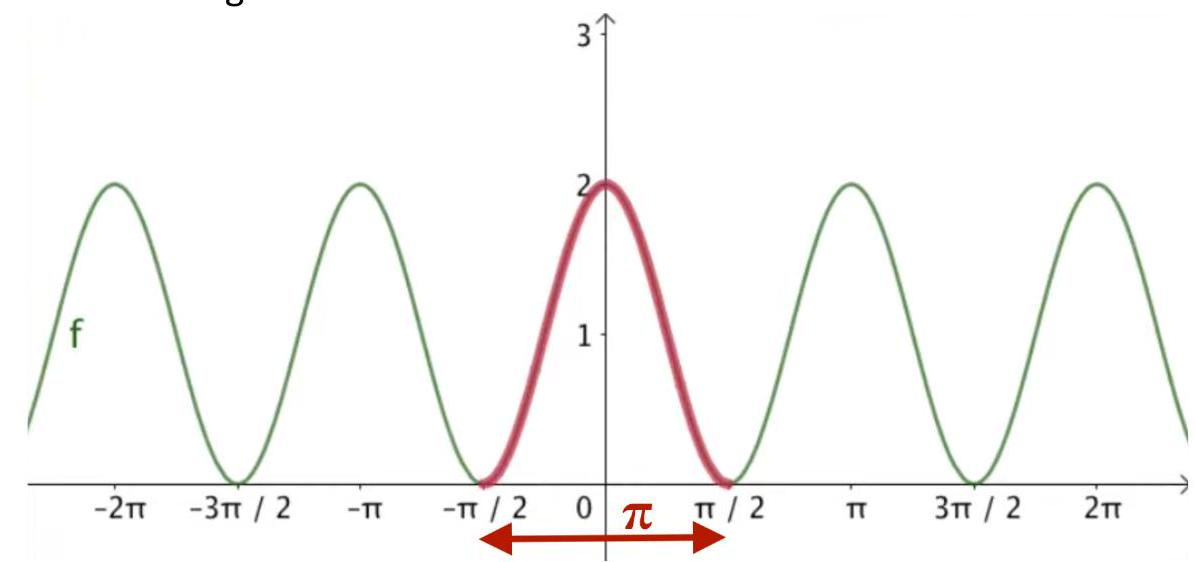
\includegraphics[scale=0.15]{2024_01_04_295cf56f03985ebac5b3g-09(3)}
     	\end{center}
     	\grasInMet{- FONCTION $g$ :}\\
     	La fonction $g$ est impaire car sa courbe est symétrique par rapport à l'origine.
     	\begin{center}
     		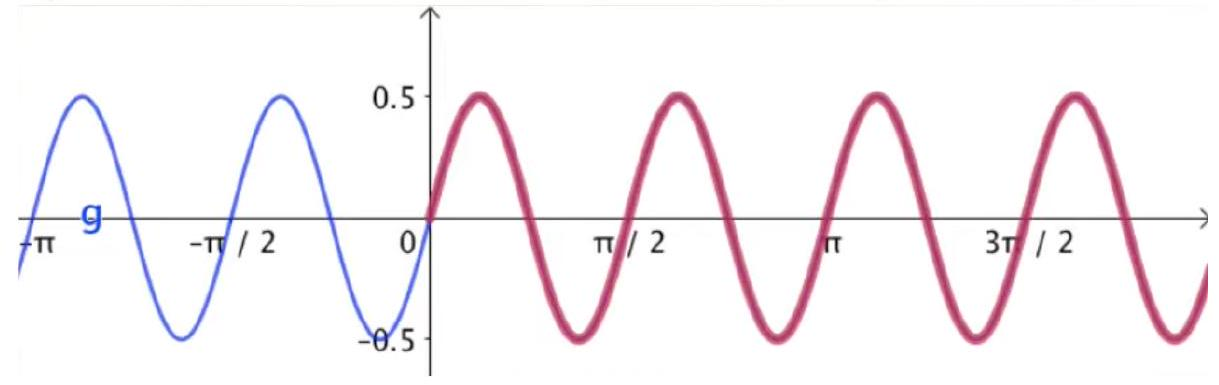
\includegraphics[scale=0.15]{2024_01_04_295cf56f03985ebac5b3g-09(1)}
     	\end{center}
     	La fonction $g$ est périodique de période $\frac{\pi}{2}$ car on retrouve le même morceau de courbe sur chaque intervalle de longueur $\frac{\pi}{2}$.
     	\begin{center}
     		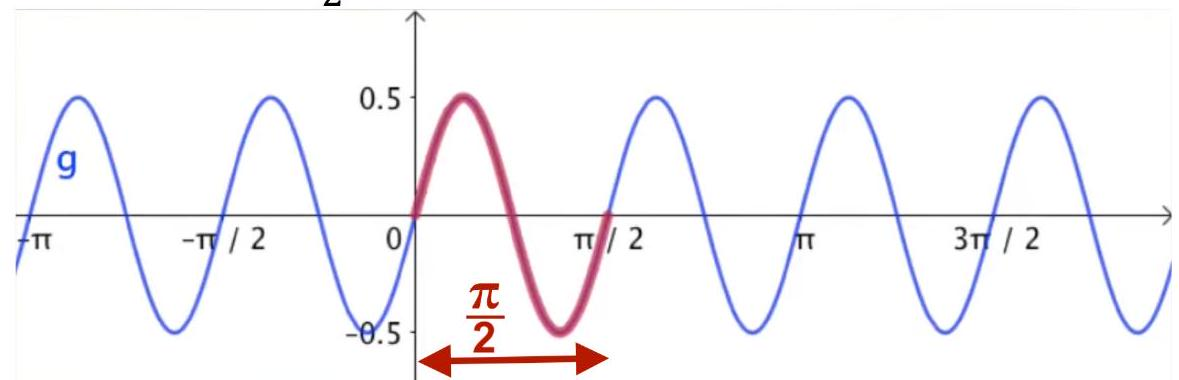
\includegraphics[scale=0.15]{2024_01_04_295cf56f03985ebac5b3g-09}
     	\end{center}
     	\grasInMet{- FONCTION $h$ :}\\
     	La fonction $h$ est paire car sa courbe est symétrique par rapport à l'axe des ordonnées.
     	\begin{center}
     		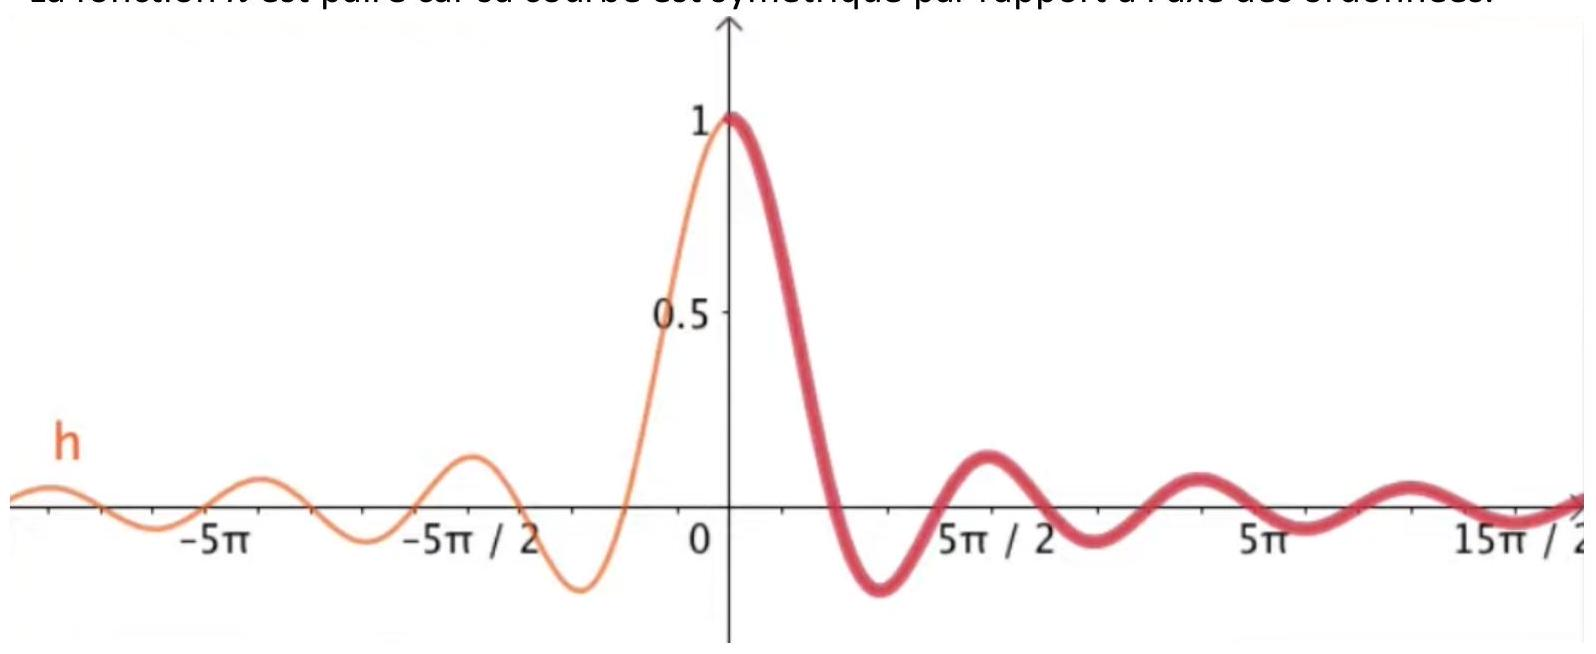
\includegraphics[scale=0.15]{2024_01_04_295cf56f03985ebac5b3g-10(1)}
     	\end{center}
     	La fonction $h$ n'est pas périodique, on ne retrouve pas le même morceau de courbe sur différents intervalles.
    \end{bmethodet}

	\begin{bmethodet}{Étudier la parité d'une fonction trigonométrique}
		\grasInMet{Enoncé:}\\
		Démontrer que la fonction $f$ définie sur $\mathbb{R} \operatorname{par} f(x)=\sin (x)-\sin (2 x)$ est impaire.\\
		\grasInMet{Corrigé:}\\
		On a :
		
		$f(-x)=\sin (-x)-\sin (-2 x)=-\sin (x)+\sin (2 x)=-(\sin (x)-\sin (2 x))=-f(x)$. La fonction $f$ est donc impaire.
		
		Sa représentation graphique est symétrique par rapport à l'origine du repère.
	\end{bmethodet}

	\begin{bmethodet}{Compléter un graphique par parité et périodicité}
		\grasInMet{Enoncé:}\\
		Soit $f$ une fonction impaire et périodique de période $\pi$. Compléter sa représentation graphique sur l'intervalle $\left[-\frac{3 \pi}{2} ; \frac{3 \pi}{2}\right]$.
		
		\begin{center}
			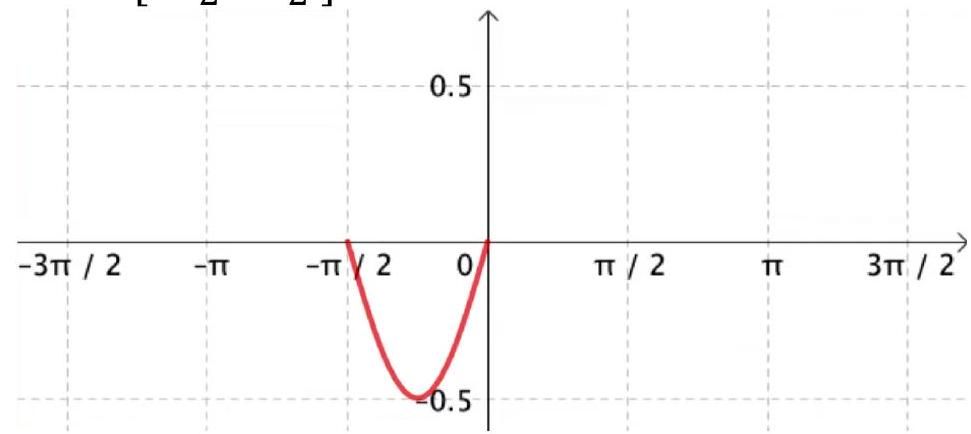
\includegraphics[scale=0.2]{2024_01_04_295cf56f03985ebac5b3g-10}
		\end{center}
		\grasInMet{Corrigé:}\\
		$1^{\text {ère }}$ étape : La fonction est impaire. Sa courbe représentative est symétrique par rapport à l'origine du repère.
		
		On complète donc par symétrie centrale.
		
		\begin{center}
			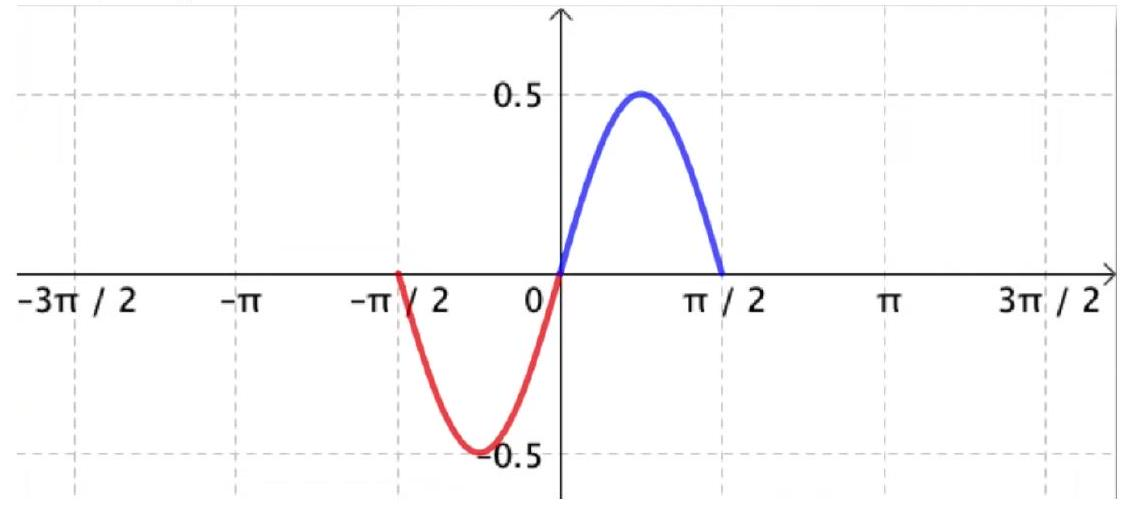
\includegraphics[scale=0.2]{2024_01_04_295cf56f03985ebac5b3g-11(1)}
		\end{center}
		
		$2^{\mathrm{e}}$ étape : La fonction est périodique de période $\pi$. On retrouve le même morceau de courbe sur chaque intervalle de longueur $\pi$.
		
		Le morceau déjà tracé a pour longueur $\pi$, on le reproduit à gauche et à droite.
		
		\begin{center}
			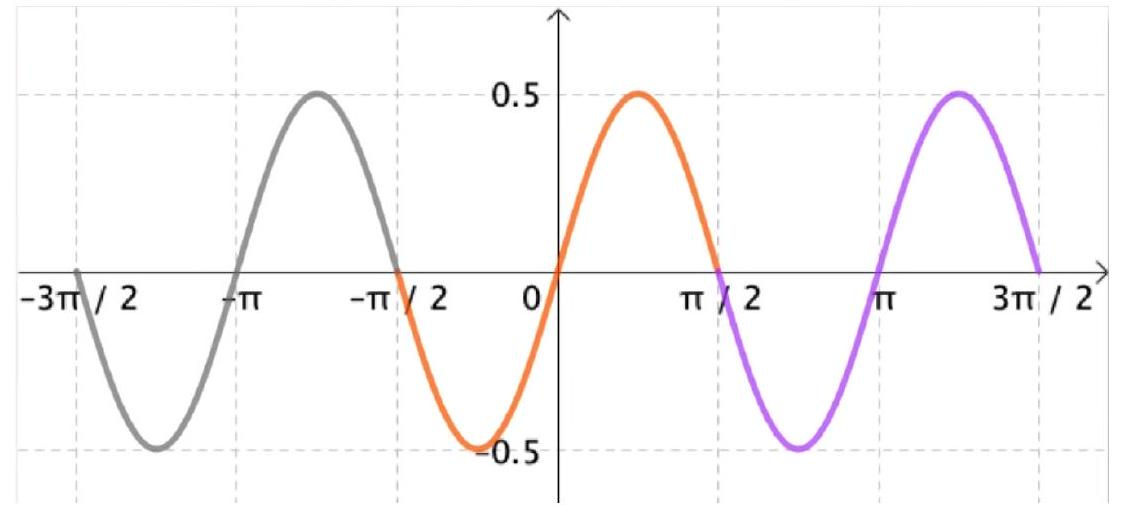
\includegraphics[scale=0.2]{2024_01_04_295cf56f03985ebac5b3g-11}
		\end{center}
	\end{bmethodet}


\graphicspath{{images/}}
\chapter{Fonctions de référence}
\thispagestyle{fancy}

\graphicspath{{images/}}

\section{Fonction carré}
    \subsection{définition}
    \begin{bdefi}
        La fonction carré $f$ est définie sur \R par $f(x)=x^2$.
    \end{bdefi}
    
    \subsection{Représentation graphique}
    
    \begin{minipage}{0.5\linewidth}
        \begin{tabular}{ | Xc | Xc | Xc | Xc | Xc | Xc |}
         \hline			
           $x$  & $-2$ & $-1$ & $0$ & $1$ & $2$\\ \hline
           $f(x)$ & $4$ & $1$ & $0$ & $1$ & $4$ \\
         \hline  
        \end{tabular}
    \end{minipage}\hfill
    \begin{minipage}{0.45\linewidth}
        \begin{center}
            \newrgbcolor{xdxdff}{0.49019607843137253 0.49019607843137253 1.}
            \newrgbcolor{ududff}{0.30196078431372547 0.30196078431372547 1.}
            \newrgbcolor{qqwuqq}{0. 0.39215686274509803 0.}
            \newrgbcolor{xfqqff}{0.4980392156862745 0. 1.}
            \psset{xunit=1.2cm,yunit=1.2cm,algebraic=true,dimen=middle,dotstyle=o,dotsize=5pt 0,linewidth=2.pt,arrowsize=2pt 2,arrowinset=0.25}
            \begin{pspicture*}(-2.5,-0.8)(2.5,5.8)
            \psgrid[xunit=1.2cm,yunit=1.2cm,subgriddiv=0,gridcolor=lightgray,gridlabels=0pt](-3,-1)(3,6)
            \psaxes[linewidth=0.6pt,labelFontSize=\scriptstyle,xAxis=true,yAxis=true,Dx=1.,Dy=1.,ticksize=-2pt 0,subticks=1]{->}(0,0)(-2.5,-0.8)(2.5,5.8)
            \psplot[linewidth=1.2pt,linecolor=qqwuqq,plotpoints=600]{-3}{3}{x^2}
            \psline[linewidth=1.2pt,linecolor=blue]{->}(0.,0.)(1.,0.)
            \psline[linewidth=1.2pt,linecolor=blue]{->}(0.,0.)(0.,1.)
            \psdots[dotstyle=x,linecolor=blue](-2.,4)
            \psdots[dotstyle=x,linecolor=blue](-1.,1.)
            \psdots[dotstyle=x,linecolor=blue](-0.5,0.25)
            \psdots[dotstyle=x,linecolor=blue](0.5,0.25)
            \psdots[dotstyle=x,linecolor=blue](1.,1.)
            \psdots[dotstyle=x,linecolor=blue](2.,4.)
            \begin{scriptsize}
            \rput[bl](0.34,-0.54){\textcolor{blue}{$\vv{i}$}}
            \rput[bl](-0.4,0.2){\textcolor{blue}{$\vv{j}$}}
            \end{scriptsize}
            \end{pspicture*}
        \end{center}
    \end{minipage}
    
    \begin{brmqs}
        \begin{itemRem}
            \item Le tableau de valeurs n'est pas un tableau de proportionnalité. La fonction carré n'est donc pas une fonction linéaire.
            \item 	Dans un repère $(O, I, J)$, la courbe d'équation $y=x^2$ de la fonction carré est appelée une \grasInRem{parabole} de sommet O.
            \item 	Dans un repère orthogonal, la courbe d'équation $y=x^2$ de la fonction carré est symétrique par rapport à l'axe des ordonnées. La fonction carré est donc une \grasInRem{fonction paire}.
        \end{itemRem}
    \end{brmqs}
    
    \subsection{Variations de la fonction carré}
    
    \begin{bprop}
        La fonction carré $f$ est décroissante sur l'intervalle $\intervOF{-\infty}{0}$ et croissante sur l'intervalle $\intervFO{0}{+\infty}$.
    \end{bprop}
    
    % \begin{demonstration}
    %     On pose : $f(x)=x^2$.\\
	   % Soit $a$ et $b$ deux nombres réels quelconques positifs tels que $a<b$.\\
    %     $f(b)-f(a)=b^2-a^2=(b-a)(b+a)$\\
    %     Or $b-a>0$, $a\geq 0$ et $b \geq 0$ donc $f(b)-f(a)\geq 0$ ce qui prouve que $f$ est croissante sur l'intervalle $\intervFO{0}{+\infty}$.\\
    %     \ \\
    % 	La décroissance sur l'intervalle $\intervOF{-\infty}{0}$ est prouvée de manière analogue en choisissant $a$ et $b$ deux nombres réels quelconques négatifs tels que $a<b$.
    % \end{demonstration}

\section{Fonction racine carrée}
    \subsection{définition}
    \begin{bdefi}
        La fonction racine carrée est la fonction $f$ définie sur $\intervFO{0}{+\infty}$ par $f(x)=\sqrt{x}$.
    \end{bdefi}
    
    \subsection{Représentation graphique}
    
    \begin{center}
            \newrgbcolor{qqwuqq}{0. 0.39215686274509803 0.}
            \psset{xunit=1.3cm,yunit=1.3cm,algebraic=true,dimen=middle,dotstyle=o,dotsize=5pt 0,linewidth=2.pt,arrowsize=2pt 2,arrowinset=0.25}
            \begin{pspicture*}(-0.5,-0.8)(9.5,3.5)
            \psgrid[xunit=1.3cm,yunit=1.3cm,subgriddiv=0,gridcolor=lightgray,gridlabels=0pt](-1,-1)(10,4)
            \psaxes[linewidth=0.6pt,labelFontSize=\scriptstyle,xAxis=true,yAxis=true,Dx=1.,Dy=1.,ticksize=-2pt 0,subticks=1]{->}(0,0)(-0.5,-0.8)(9.5,3.5)
            \psplot[linewidth=1.2pt,linecolor=qqwuqq,plotpoints=600]{0}{10}{sqrt(x)}
            \psline[linewidth=1.2pt,linecolor=blue]{->}(0.,0.)(1.,0.)
            \psline[linewidth=1.2pt,linecolor=blue]{->}(0.,0.)(0.,1.)
            \begin{scriptsize}
            \rput[bl](0.34,-0.54){\textcolor{blue}{$\vv{i}$}}
            \rput[bl](-0.4,0.2){\textcolor{blue}{$\vv{j}$}}
            \end{scriptsize}
            \end{pspicture*}
    \end{center}
    
    
    \begin{brmq}
        La fonction racine carrée n'est pas définie pour des valeurs négatives.
    \end{brmq}
    
    \subsection{Variations de la fonction racine carrée}
    
    \begin{bprop}
        La fonction racine carrée est strictement croissante sur l'intervalle $\intervFO{0}{+\infty}$.
    \end{bprop}
    
    \begin{bdemo}
        On pose : $f(x)=\sqrt{x}$.\\
        Soit $a$ et $b$ deux nombres réels positifs tels que $a < b$.\\
        $f(b)-f(a)=\sqrt{b}-\sqrt{a}=  \dfrac{(\sqrt{b}-\sqrt{a})(\sqrt{b}+\sqrt{a})}{\sqrt{b}+\sqrt{a}}=\dfrac{\sqrt{b}^2-\sqrt{a}^2}{\sqrt{b}+\sqrt{a}} = \dfrac{b-a}{\sqrt{b}+\sqrt{a}}$.\\
        Or $\sqrt{b}+\sqrt{a}  > 0$ et $b - a > 0$. Donc $f(b)-f(a)>0$
        Donc $f(a)<f(b)$.\\
        Ce qui prouve que $f$ est croissante sur l'intervalle $\intervFO{0}{+\infty}$.
    \end{bdemo}
    
\section{Fonction inverse}
    \subsection{définition}
    \begin{bdefi}
        La fonction inverse $f$ est définie sur $\R\textbackslash\{0\}$ par $f(x)= \dfrac{1}{x}$.
    \end{bdefi}
    
    \begin{brmqs}
        \begin{itemRem}
            \item $\R\textbackslash\{0\}$ désigne l'ensemble des nombres réels sauf 0, c'est-à-dire 
            $\intervOO{-\infty}{0}\  \cup \  \intervOO{0}{+\infty}$. On peut aussi noter cet ensemble $\R^*$.
            \item La fonction inverse n'est pas définie en 0.
        \end{itemRem}
    \end{brmqs}
    
    \subsection{Représentation graphique}
    
    \setlength{\tabcolsep}{0.25cm}
    \begin{minipage}{0.4\linewidth}
        \begin{tabular}{ | Xc | Xc | Xc | Xc | Xc | Xc | Xc |}
         \hline			
           $x$  & $-2$ & $-1$ & $0,25$ & $1$ & $2$ & $3$\\ \hline
           $f(x)$ & $-0,5$ & $-1$ & $4$ & $1$ & $0,5$ & $\dfrac{1}{3}$ \\
         \hline  
        \end{tabular}
    \end{minipage}\hfill
    \begin{minipage}{0.55\linewidth}
        \begin{center}
            \newrgbcolor{xdxdff}{0.49019607843137253 0.49019607843137253 1.}
            \newrgbcolor{ududff}{0.30196078431372547 0.30196078431372547 1.}
            \newrgbcolor{qqwuqq}{0. 0.39215686274509803 0.}
            \newrgbcolor{xfqqff}{0.4980392156862745 0. 1.}
            \psset{xunit=0.9cm,yunit=0.9cm,algebraic=true,dimen=middle,dotstyle=o,dotsize=5pt 0,linewidth=2.pt,arrowsize=2pt 2,arrowinset=0.25}
            \begin{pspicture*}(-3.9,-3.2)(4.3,4.2)
            \psgrid[xunit=0.9cm,yunit=0.9cm,subgriddiv=0,gridcolor=lightgray,gridlabels=0pt](-4,-4)(5,5)
            \psaxes[linewidth=0.6pt,labelFontSize=\scriptstyle,xAxis=true,yAxis=true,Dx=1.,Dy=1.,ticksize=-2pt 0,subticks=1]{->}(0,0)(-3.9,-3.2)(4.3,4.2)
            \psplot[linewidth=1.2pt,linecolor=qqwuqq,plotpoints=600]{-4}{-0.01}{1/x}
            \psplot[linewidth=1.2pt,linecolor=qqwuqq,plotpoints=600]{0.01}{5}{1/x}
            \psline[linewidth=1.2pt,linecolor=blue]{->}(0.,0.)(1.,0.)
            \psline[linewidth=1.2pt,linecolor=blue]{->}(0.,0.)(0.,1.)
            \psdots[dotstyle=x,linecolor=blue](-3.,-0.3333)
            \psdots[dotstyle=x,linecolor=blue](-2.,-0.5)
            \psdots[dotstyle=x,linecolor=blue](-1.,-1.)
            \psdots[dotstyle=x,linecolor=blue](0.25,4.)
            \psdots[dotstyle=x,linecolor=blue](1.,1.)
            \psdots[dotstyle=x,linecolor=blue](2.,0.5)
            \psdots[dotstyle=x,linecolor=blue](3.,0.3333)
            \psdots[dotstyle=x,linecolor=blue](4.,0.25)
            \begin{scriptsize}
            \rput[bl](0.34,-0.54){\textcolor{blue}{$\vv{i}$}}
            \rput[bl](-0.4,0.2){\textcolor{blue}{$\vv{j}$}}
            \end{scriptsize}
            \end{pspicture*}
        \end{center}
    \end{minipage}
    
    \begin{brmqs}
        \begin{itemRem}
            \item Dans un repère $(O, I, J)$, la courbe d'équation $y= \dfrac{1}{x}$  de la fonction inverse est une \grasInRem{hyperbole} de centre O.
            \item 	La courbe d'équation $y= \dfrac{1}{x}$ de la fonction inverse est symétrique par rapport à l'origine. La fonction inverse est donc une \grasInRem{fonction impaire}.
        \end{itemRem}
    \end{brmqs}
    
    \subsection{Variations de la fonction inverse}
    
    \begin{bprop}
        La fonction inverse est décroissante sur l'intervalle $\intervOO{-\infty}{0}$  et décroissante sur l'intervalle $\intervOO{0}{+\infty}$.
    \end{bprop}
    
    \begin{brmq}
        La variation d'une fonction ne peut s'étudier que sur un intervalle. \\
        On ne peut donc pas évoquer de décroissance sur $\intervOO{-\infty}{0}\  \cup \  \intervOO{0}{+\infty}$ qui n'est pas un intervalle mais conclure de manière séparée que la fonction inverse est décroissante sur l'intervalle $\intervOO{-\infty}{0}$ et décroissante sur l'intervalle $\intervOO{0}{+\infty}$.
    \end{brmq}
    
    % \begin{demonstration}
    %     On pose : $f(x)= \dfrac{1}{x}$.\\
    %     Soit $a$ et $b$ deux nombres réels strictement positifs avec $a < b$.\\ 
    %     $f(b)-f(a)= \dfrac{1}{b} - \dfrac{1}{a} = \dfrac{a-b}{ab}$.\\
    %     Or $a > 0$, $b  > 0$ et $a – b < 0$. Donc $f(b)-f(a)\leq 0$.\\
    %     $f$ est ainsi décroissante sur l'intervalle $\intervOO{0}{+\infty}$.\\
    %     \ \\
    %     La décroissance sur l'intervalle $\intervOO{-\infty}{0}$  est prouvée de manière analogue.
    % \end{demonstration}
    
\section{Fonction cube}
    \subsection{définition}
    \begin{bdefi}
        La fonction cube est la fonction $f$ définie sur \R par $f(x)=x^3$.
    \end{bdefi}
    
    \subsection{Représentation graphique}
    
    \begin{center}
        \newrgbcolor{xdxdff}{0.49019607843137253 0.49019607843137253 1.}
        \newrgbcolor{ududff}{0.30196078431372547 0.30196078431372547 1.}
        \newrgbcolor{qqwuqq}{0. 0.39215686274509803 0.}
        \newrgbcolor{xfqqff}{0.4980392156862745 0. 1.}
        \psset{xunit=1.2cm,yunit=1.2cm,algebraic=true,dimen=middle,dotstyle=o,dotsize=5pt 0,linewidth=2.pt,arrowsize=2pt 2,arrowinset=0.25}
        \begin{pspicture*}(-2.5,-3.2)(2.5,3.2)
        \psgrid[xunit=1.2cm,yunit=1.2cm,subgriddiv=0,gridcolor=lightgray,gridlabels=0pt](-3,-4)(3,4)
        %\psgrid[gridwidth=0.1pt,gridcolor=lightgray,gridlabels=0](0,0)(-4.,-2.)(4.5,5.5)
        \psaxes[linewidth=0.6pt,labelFontSize=\scriptstyle,xAxis=true,yAxis=true,Dx=1.,Dy=1.,ticksize=-2pt 0,subticks=1]{->}(0,0)(-2.5,-3.2)(2.5,3.2)
        \psplot[linewidth=1.2pt,linecolor=qqwuqq,plotpoints=600]{-3}{3}{x^(3.0)}
        \psline[linewidth=1.2pt,linecolor=blue]{->}(0.,0.)(1.,0.)
        \psline[linewidth=1.2pt,linecolor=blue]{->}(0.,0.)(0.,1.)
        \begin{scriptsize}
        \rput[bl](0.34,-0.54){\textcolor{blue}{$\vv{i}$}}
        \rput[bl](-0.4,0.2){\textcolor{blue}{$\vv{j}$}}
        \end{scriptsize}
        \end{pspicture*}
    \end{center}
    
    \begin{brmq}
        Dans un repère orthogonal, la courbe d'équation $y=x^3$ de la fonction cube est symétrique par rapport au centre du repère. La fonction cube est donc une \grasInRem{fonction impaire}.
    \end{brmq}
    
    \subsection{Variations de la fonction cube}
    
    \begin{bprop}
        La fonction cube est strictement croissante sur \R.
    \end{bprop}
    
    Cette propriété est admise.
\chapter{Dérivation}
\thispagestyle{fancy}

\section{Limite en zéro d'une fonction}

\begin{bexemples}
    \begin{enumEx}
        \item Soit la fonction $f$ définie sur $\left]-\infty ; 0\right[\cup\left] 0 ;+\infty\right[ $ par $f(x)=\dfrac{(x+1)^{2}-1}{x}$. \\
        L'image de 0 par la fonction $f$ n'existe pas. On s'intéresse cependant aux valeurs de $f(x)$ lorsque $x$ se rapproche de $0$.
        \begin{center}
            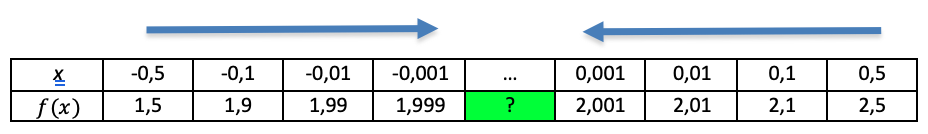
\includegraphics[scale=1]{01-05-Img01}
        \end{center}
        On constate que $f(x)$ se rapproche de 2 lorsque $x$ se rapproche de 0 . On dit que la limite de $f$ lorsque $x$ tend vers 0 est égale à 2 et on note : $\lim \limits_{x \rightarrow 0} f(x)=2$.
        \item Soit la fonction $g$ définie sur $]-\infty ; 0[\cup] 0 ;+\infty[$ par $g(x)=\dfrac{1}{x^{2}}$.\\
        A l'aide de la calculatrice, on constate que $g(x)$ devient de plus en plus grand lorsque $x$ se rapproche de 0
        On dit que la limite de $g$ lorsque $x$ tend vers 0 est égale à $+\infty$ et on note :
        $\lim \limits_{x \rightarrow 0} g(x)=+\infty$
    \end{enumEx}
\end{bexemples}

\begin{bdefi}
    On dit que $f(x)$ a pour limite $L$ lorsque $x$ tend vers 0 si les valeurs de $f(x)$ peuvent être aussi proche de $L$ que l'on veut pourvu que $x$ soit suffisamment proche de 0 . \\
    On note $: \lim \limits_{x \rightarrow 0} f(x)=L$ et on lit : La limite de $f(x)$ lorsque $x$ tend vers 0 est égale à $L$.
\end{bdefi}

\section{Nombre dérivé}

\subsection{Rappel : Pente d'une droite}

Soit une fonction $f$ définie sur un intervalle I. Soit deux réels $a$ et $b$ appartenant à I tels que $a<b$. Soit $\mathrm{A}$ et $\mathrm{B}$ deux points de la courbe représentative de $f$ d'abscisses respectives $a$ et $b$. La pente (ou le coefficient directeur) de la droite (AB) est égal à : $\dfrac{f(b)-f(a)}{b-a}$.

\begin{center}
    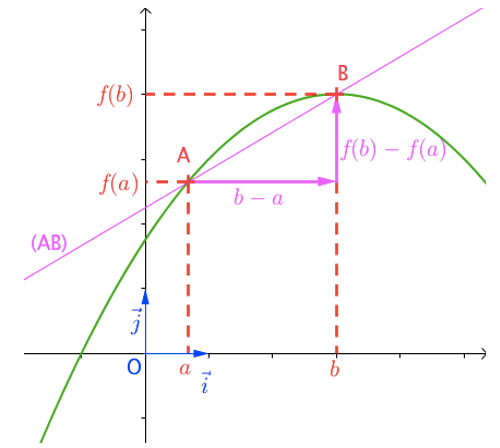
\includegraphics[scale=0.8]{01-05-Img02}
\end{center}

\subsection{Fonction dérivable}

\begin{multicols}{2}

Soit une fonction $f$ définie sur un intervalle $I .$ Soit un réel $a$ appartenant à I.\\
\ \\
Soit A et M deux points de la courbe représentative de $f$ d'abscisses respectives $a$ et $a+h,$ avec $h \neq 0$
La pente de la droite (AM) est égale à :
$\dfrac{f(a+h)-f(a)}{a+h-a}=\dfrac{f(a+h)-f(a)}{h}$.\\

Lorsque le point $M$ se rapproche du point $A$, la pente de la droite (AM) est égale à la limite de $\dfrac{f(a+h)-f(a)}{h}$ lorsque $h$ tend vers 0.\\
Cette pente s'appelle le nombre dérivé de $f$ en $a$ et se note $f^{\prime}(a)$.

\columnbreak

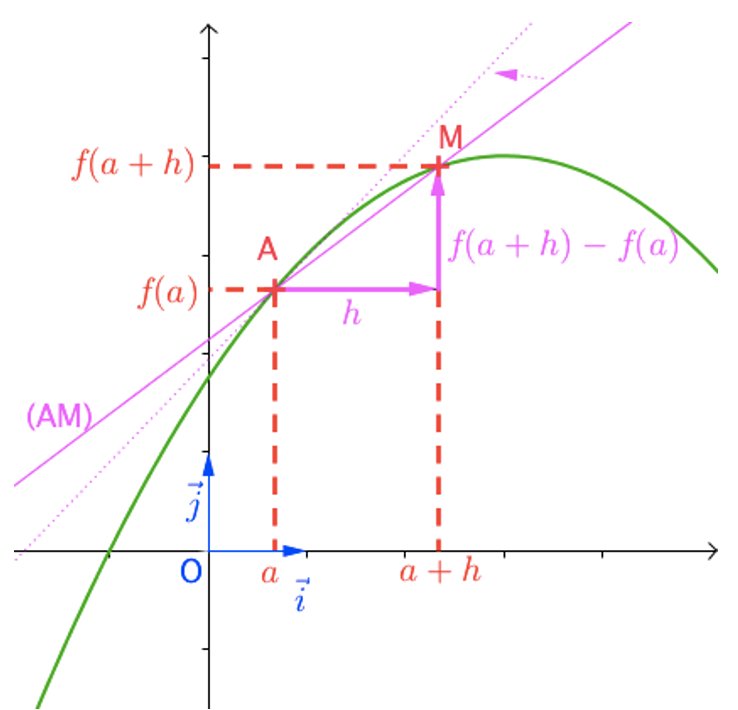
\includegraphics[scale=0.6]{01-05-Img03}

\end{multicols}

\begin{definition}
On dit que la fonction $f$ est dérivable en $a$ s'il existe un nombre réel $L$, tel que :
$$
\lim _{h \rightarrow 0} \frac{f(a+h)-f(a)}{h}=L
$$
L est appelé le nombre dérivé de $f$ en $a$ et se note $f^{\prime}(a)$.
\end{definition}

\subsection{Démontrer qu'une fonction est dérivable}

\begin{bmethode}
    Soit la fonction trinôme $f$ définie sur $\mathbb{R}$ par $f(x)=x^{2}+2x-3$
    Démontrer que $f$ est dérivable en $x=2$.
    On commence par calculer $\dfrac{f(2+h)-f(2)}{h}$ pour $h \neq 0$\\
    
    $\begin{aligned}
        \frac{f(2+h)-f(2)}{h}&=\frac{(2+h)^{2}+2(2+h)-3-2^{2}-2 \times 2+3}{h} \\
        &=\frac{4+4 h+h^{2}+4+2 h-8}{h} \\
        &=\frac{6 h+h^{2}}{h} \\
        &=\frac{h(6+h)}{h} \\
        &=6+h
    \end{aligned}$
    
    Donc $: \lim \limits_{h \rightarrow 0} \dfrac{f(2+h)-f(2)}{h}=\lim \limits_{h \rightarrow 0} 6+h=6$.\\
    On en déduit que $f$ est dérivable en $x=2$. Le nombre dérivé de $f$ en 2 vaut 6 et on note $: f^{\prime}(2)=6$.
\end{bmethode}

\section{Tangente à une courbe}

\subsection{Définition}

\begin{multicols}{2}
Soit une fonction $f$ définie sur un intervalle I et dérivable en un nombre réel $a$ appartenant à I.\\
$f^{\prime}(a)$ est le nombre dérivé de $f$ en $a$.\\
A est un point d'abscisse $a$ appartenant à la courbe représentative $C_{f}$ de $f$.

\begin{bdefi}
    La tangente à la courbe $C_{f}$ au point $\mathrm{A}$ est la droite passant par $\mathrm{A}$ de pente le nombre dérivé $f^{\prime}(a)$.
\end{bdefi}

\columnbreak

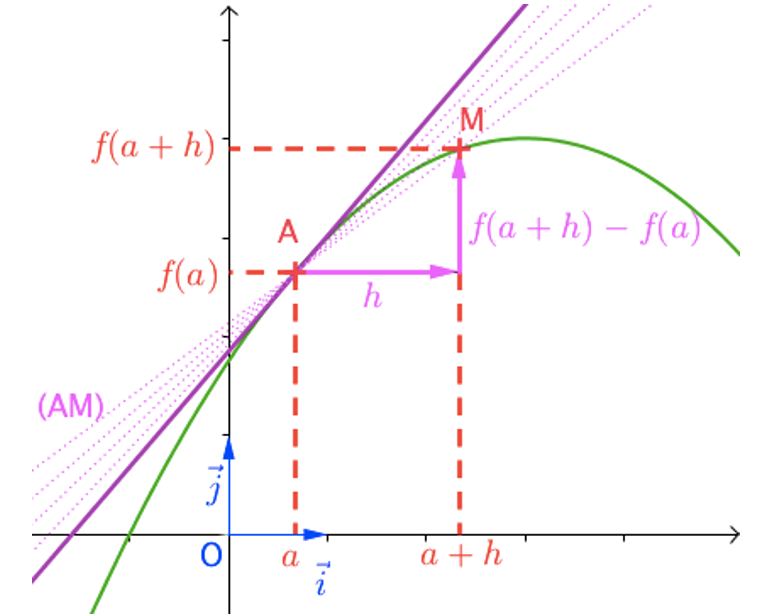
\includegraphics[scale=0.55]{01-05-Img04}
\end{multicols}

\subsection{Déterminer le coefficient directeur d'une tangente à une courbe}

\begin{bmethode}
    On considère la fonction trinôme $f$ définie sur $\mathbb{R}$ par $f(x)=x^{2}+2 x-3$ dont la dérivabilité en 2 a été étudiée plus haut.\\
    Déterminer la pente de la tangente à la courbe représentative de $f$ au point $\mathrm{A}$ de la courbe d'abscisse $2$.\\
    On a vu que le nombre dérivé de $f$ en 2 vaut 6 . Ainsi la tangente à la courbe représentative de $f$ au point $A$ de la courbe d'abscisse 2 est la droite passant par $\mathrm{A}$ et de pente (coefficient directeur) 6.
    \begin{center}
        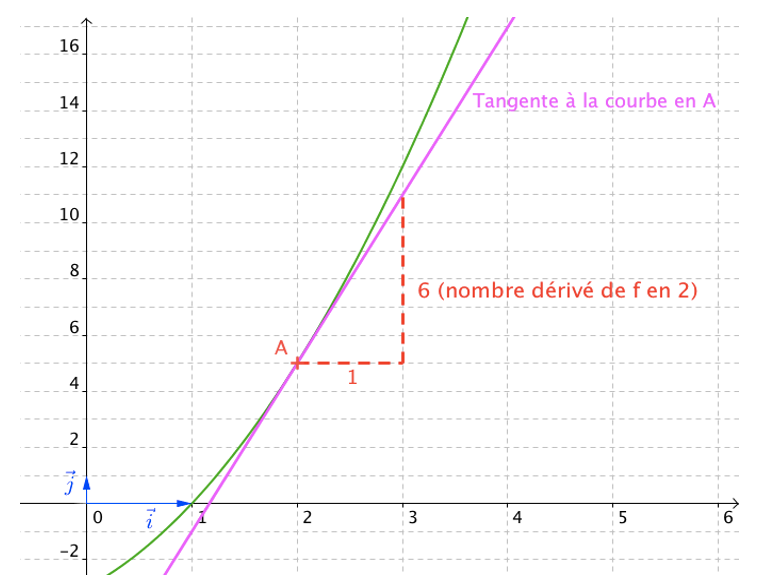
\includegraphics[scale=0.85]{01-05-Img05}
    \end{center}
\end{bmethode}

\subsection{Relation entre tangente et nombre dérivée}

\begin{bprop}
Une équation de la tangente à la courbe $C_{f}$ en A est :
$$
y=f^{\prime}(a)(x-a)+f(a)
$$
\end{bprop}

\begin{bdemo}
    La tangente a pour pente $f^{\prime}(a)$ donc son équation est de la forme $: y=f^{\prime}(a) x+b$ où $b$ est l'ordonnée à l'origine.\\
    \ \\
    Déterminons $b$ :\\
    La tangente passe par le point $\mathrm{A}(a ; f(a)),$ donc:\\
    $f(a)=f^{\prime}(a) \times a+b$ soit $: b=f(a)-f^{\prime}(a) \times a$\\
    On en déduit que l'équation de la tangente peut s'écrire :\\
    $y=f^{\prime}(a) x+f(a)-f^{\prime}(a) \times a$\\
    $y=f^{\prime}(a)(x-a)+f(a)$\\
\end{bdemo}

\subsection{Déterminer une équation d'une tangente à une courbe}

\begin{bmethode}
    On considère la fonction trinôme $f$ définie sur $\mathbb{R}$ par $f(x)=x^{2}+2 x-3$.\\ Déterminer une équation de tangente à la courbe représentative de $f$ au point $\mathrm{A}$ de la courbe d'abscisse 2 .\\
    On a vu plus haut que la pente de la tangente est égal à 6 . Donc son équation est de la forme $: y=6(x-2)+f(2),$ soit :\\
    $y=6(x-2)+2^{2}+2 \times 2-3$\\
    $y=6 x-7$\\
    Une équation de tangente à la courbe représentative de $f$ au point $\mathrm{A}$ de la courbe d'abscisse 2 est $y=6 x-7$.
\end{bmethode}

\section{Dérivées des fonctions usuelles}

\subsection{Exemple (démonstration au programme)}
\begin{bdemo}
    Soit la fonction $f$ définie sur \R par $f(x)=x^2$.\\ 
    Démontrons que pour tout x réel, on a:\\
    $f'(x)=2x$.


Calculons le nombre dérivé de la fonction $f$ en un nombre réel quelconque $a$. 
\[ \text{Pour }h\neq0:\frac{f(a+h)-f(a)}{h}=\frac{(a+h)^2-a^2}{h}=\frac{a^2+2ah+h^2-a^2}{h}=\frac{h(2a+h)}{h}=2a+h\]
\[ \text{Or }:\lim\limits_{h \rightarrow 0} \frac{f(a+h)-f(a)}{h} = \lim\limits_{h \rightarrow 0} 2a+h=2a\]

Pour tout nombre $a$, on associe le nombre dérivé de la fonction $f$ égal à $2a$.
On a donc défini sur \R une fonction, notée $f'$ dont l'expression est $f'(x)=2x$.
Cette fonction s'appelle la fonction dérivée de $f$.
\end{bdemo}

\begin{bdefi}
    Soit $f$ une fonction définie sur un intervalle I.
    On dit que $f$ est dérivable sur I si elle est dérivable en tout réel $x$ de I.
    Dans ce cas, la fonction qui à tout réel $x$ de I associe le nombre dérivé de $f$ en $x$ est appelée fonction dérivée de $f$ et se note $f'$.
\end{bdefi}

\subsection{Formules de dérivation des fonctions usuelles}

% \begin{center}
%     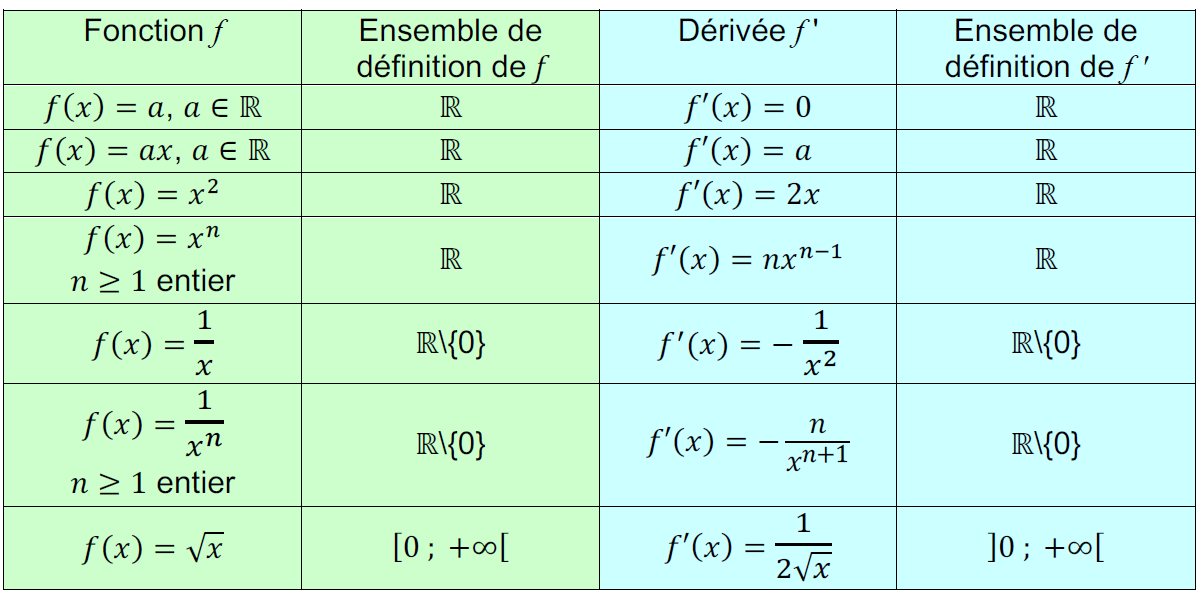
\includegraphics[scale=0.5]{01-06-01}
% \end{center}

\setlength{\arrayrulewidth}{1pt}
\renewcommand{\arraystretch}{1.9}
    \begin{tabular}{| >{\columncolor{green!25!white}}C{4cm} | >{\columncolor{green!25!white}}C{3cm} | >{\columncolor{cyan!25!white}}C{4cm} | >{\columncolor{cyan!25!white}}C{3cm} |}
\hline Fonction $f$ & Ensemble de\newline définition de $f$ & Dérivée $f^{\prime}$ & Ensemble de\newline définition de $f^{\prime}$ \\
\hline$f(x)=a$, $a \in \mathbb{R}$ & $\mathbb{R}$ & $f^{\prime}(x)=0$ & $\mathbb{R}$ \\
\hline$f(x)=a x$, $a \in \mathbb{R}$ & $\mathbb{R}$ & $f^{\prime}(x)=a$ & $\mathbb{R}$ \\
\hline$f(x)=x^{2}$ & $\mathbb{R}$ & $f^{\prime}(x)=2 x$ & $\mathbb{R}$ \\
\hline$f(x)=x^{n}$\newline $n \geqslant 1$ entier & $\mathbb{R}$ & $f^{\prime}(x)=n x^{n-1}$ & $\mathbb{R}$ \\
\hline$f(x)=\dfrac{1}{x}$ & $\mathbb{R} \backslash\{0\}$ & $f^{\prime}(x)=-\dfrac{1}{x^{2}}$ & $\mathbb{R} \backslash\{0\}$\rule[-7pt]{0pt}{30pt} \\
\hline$f(x)=\dfrac{1}{x^{n}}$\newline$n \geqslant 1$ entier & $\mathbb{R} \backslash\{0\}$ & $f^{\prime}(x)=-\dfrac{n}{x^{n+1}}$ & $\mathbb{R} \backslash\{0\}$ \\
\hline$f(x)=\sqrt{x}$ & {$[0 ;+\infty[$} & $f^{\prime}(x)=\dfrac{1}{2 \sqrt{x}}$ & ] $0 ;+\infty[$ \\
\hline
\end{tabular}

\begin{bexemples}
\begin{enumEx}
    \item Soit la fonction $f$ définie sur \R par $f(x)=x^4$ alors $f$ est dérivable sur \R et on a pour tout $x$ de \R, $f'(x)=4x^3$.
    \item Soit la fonction $f$ définie sur $\R \backslash \lbrace 0 \rbrace$ par $f(x)=\dfrac{1}{x^5}$ alors $f$ est dérivable sur $]-\infty ; 0[$ et sur $]0 ; +\infty[$ et on a pour tout $x$ de $\R \backslash \lbrace 0 \rbrace$, $f'(x)=-\dfrac{5}{x^6}$.
\end{enumEx}
\end{bexemples}

\subsection{Démonstration au programme pour la fonction inverse}

\begin{bdemo}
    Soit la fonction $f$ définie sur $\R \backslash \lbrace 0 \rbrace$ par $f(x)= \frac{1}{x}$. Démontrons que pour tout $x$ de $\R \backslash \lbrace 0 \rbrace$, on a : $f'(x)= -\frac{1}{x^2}$.\\
    Pour $h\neq0$ et $a\neq0$:\\
    \[ \frac{f(a+h)-f(a)}{h}=\frac{\frac{1}{a+h}-\frac{1}{a}}{h}=\frac{\frac{a-a-h}{a(a+h)}}{h}=\frac{\frac{-h}{a(a+h)}}{h}=-\frac{1}{a(a+h)}\]
    \[ \text{Or }:\lim\limits_{h \rightarrow 0} \frac{f(a+h)-f(a)}{h} = \lim\limits_{h \rightarrow 0} -\frac{1}{a(a+h)}=-\frac{1}{a^2}\]
    Pour tout nombre $a$, on associe le nombre dérivé de la fonction $f$ égal à $-\frac{1}{a^2}$.\\
    Ainsi, pour tout $x$ de $\R \backslash \lbrace 0 \rbrace$, on a : $f'(x)= -\frac{1}{x^2}$.
\end{bdemo}


\subsection{Démonstration au programme : Non dérivabilité de la fonction racine carrée en 0}

\begin{bdemo}
    Soit la fonction $f$ définie sur $[0 ; +\infty[$ par $f(x)=\sqrt(x)$.\\
    On calcule le taux de variation de $f$ en $0$ :
    \[ \text{Pour }h>0:\frac{f(0+h)-f(0)}{h}=\frac{\sqrt{0+h}-\sqrt{0}}{h}=\frac{\sqrt{h}}{h}=\frac{\sqrt{h}\sqrt{h}}{h\sqrt{h}}=\frac{h}{h\sqrt{h}}=\frac{1}{\sqrt{h}}\]
    \[ \text{Or }:\lim\limits_{h \rightarrow 0} \frac{f(0+h)-f(0)}{h} = \lim\limits_{h \rightarrow 0} \frac{1}{\sqrt{h}}=+\infty\]
    \begin{minipage}{0.55\linewidth}
    En effet, lorsque $h$ tend vers $0$, $\dfrac{1}{\sqrt{h}}$  prend des valeurs de plus en plus grandes.
    Donc $f$ n'est pas dérivable en $0$.
    Géométriquement, cela signifie que la courbe représentative de la fonction racine carrée admet une tangente verticale en 0.
    \end{minipage}\hfill
    \begin{minipage}{0.4\linewidth}
    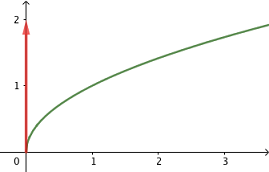
\includegraphics[scale=0.8]{01-06-02}
    \end{minipage}
\end{bdemo}

\section{Opérations sur les fonctions dérivées}
\subsection{Somme, produit, inverse, quotient de dérivées}
\begin{bexemple}
    Soit la fonction $f$ définie sur \R par  $f(x)=x+x^2$.\\
    Pour $h\neq0$:\\ 
    \begin{align*}
    	\frac{f(a+h)-f(a)}{h}&=\frac{a+h+(a+h)^2-a-a^2}{h}\\
    	&=\frac{a+h+a^2+2ah+h^2-a-a^2}{h}\\
    	&=\frac{h+2ah+h^2}{h}=1+2a+h\\
    	&=1+2a+h\\
    \end{align*}
    \[ \text{Donc }:\lim\limits_{h \rightarrow 0} \frac{f(a+h)-f(a)}{h} = \lim\limits_{h \rightarrow 0} 1+2a+h=1+2a\]
    \\
    Alors $f$ est dérivable sur \R et on a pour tout $x$ de \R, $f'(x)=1+2x$.\\
    \\
    On pose pour tout $x$ de \R, $u(x)=x$ et $v(x)=x^2$. On a ainsi : $f(x)=u(x)+v(x)$.\\
    Pour tout $x$ de \R, $u'(x)=1$ et $v'(x)=2x$.\\
    On constate sur cet exemple que : $f'(x)=u'(x)+v'(x)$. Soit encore : $(u+v)'(x)=u'(x)+v'(x)$.
\end{bexemple}
\subsubsection{Formules d'opération sur les fonctions dérivées}
u et v sont deux fonctions dérivables sur un intervalle I.
%\begin{center}
%    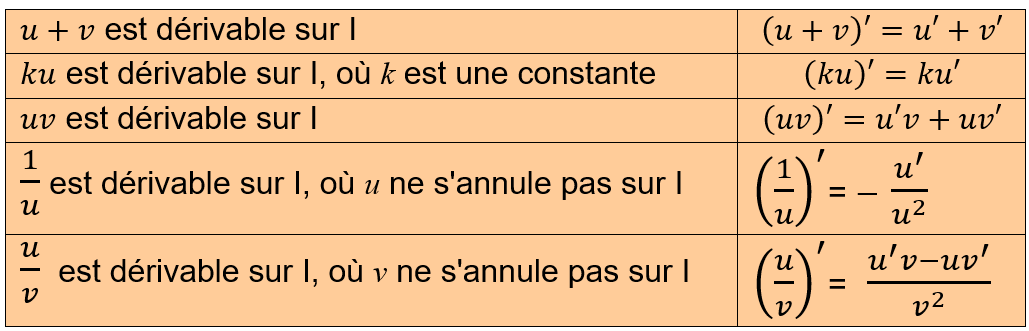
\includegraphics[scale=0.6]{01-06-03}
%\end{center}

\begin{center}
	%    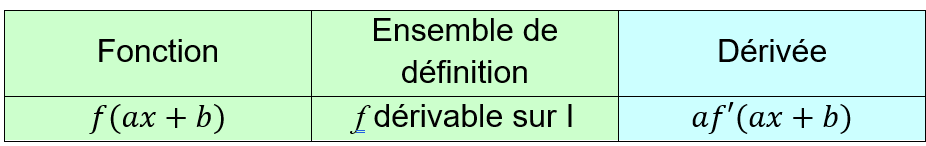
\includegraphics[scale=0.6]{01-06-04}
	\setlength{\arrayrulewidth}{1pt}
	\renewcommand{\arraystretch}{2.5}
	\begin{tabular}{| >{\columncolor{orange!25!white}}C{10cm} | >{\columncolor{orange!25!white}}C{5cm} | }
		\hline$u+v$ est dérivable sur I & $(u+v)'=u'+v'$ \\
		\hline$ku$ est dérivable sur I, où $k$ constante & $(ku)'=ku'$ \\
		\hline$uv$ est dérivable sur I & $(uv)'=u'v+uv'$ \\
		\hline$\dfrac{1}{u}$ est dérivable sur I, où $u$ ne s'annule pas sur I & $\left(\dfrac{1}{u}\right)'=-\dfrac{u'}{u^2}$ \\
		\hline$\dfrac{u}{v}$ est dérivable sur I, où $v$ ne s'annule pas sur I & $\left(\dfrac{u}{v}\right)'=\dfrac{u'v-uv'}{v^2}$ \\
		\hline
	\end{tabular}
\end{center}

\subsubsection{démonstration : Fonction dérivée d'un produit}
La démonstration sera faite en classe avec l'exercice 98 p 128.

\subsection{Calculer les dérivées de sommes, produits et quotients de fonctions}

\begin{bmethode}
Calculer les fonctions dérivées des fonctions suivantes :
\[\mBleu{1)}\ f_1(x)=5x^3\ \ \ \ \ \ \ \ \ \ \ \ \ \ \ \ \ \ \ \ \ \ \ \ \ \ \mBleu{2)} f_2(x)=3x^2+4\sqrt{x}\]
\[\mBleu{3)}\  f_3(x)=\dfrac{1}{2x^2+5x}\ \ \ \ \ \ \ \ \  \ \ \ \ \ \ \ \ \ \ \ \ \ \ \mBleu{4)}\ f_4 (x)=(3x^2+4x)(5x-1)\]

\begin{enumMet}
	\item  $f_1(x)=5u(x)$ avec $u(x)=x^3 \rightarrow u'(x)=3x^2$\\
	Donc : $f_1'(x)=5u'(x)=5\times 3x^2=15x^2$.\\
	\item $f_2(x)=u(x)+v(x)$ avec :\\
	$u(x)=3x^2 \rightarrow u'(x)=6x$\\
	$v(x)=4\sqrt{x} \rightarrow v'(x)=4\times \dfrac{1}{2\sqrt{x}}= \dfrac{2}{\sqrt{x}}$\\			
	$\text{Donc }: f_2'(x)=u'(x)+v'(x) = 6x + \dfrac{2}{\sqrt{x}}$\\
	\item $f_3(x)=\dfrac{1}{u(x)}$ avec $u(x)=2x^2+5x \rightarrow u'(x)=4x+5$\\
	Donc : $f_3'(x)= - \dfrac{u'(x)}{u(x)^2}= -\dfrac{4x+5}{(2x^2+5x)^2}$\\
	\item $f_4(x)=u(x)v(x)$ avec $u(x)=3x^2+4x \rightarrow u'(x)=6x+4$\\
	$v(x)=5x-1 \rightarrow v'(x)=5$\\			
	Donc : $f_4'(x)=u'(x)v(x)+u(x)v'(x) = (6x+4)(5x-1) + (3x^2+4x )\times 5$\\
	$=30x^2-6x+20x-4+15x^2+20x$\\
	$=45x^2+34x-4$\\
\end{enumMet}
\end{bmethode}


\subsection{Composée de dérivées}
\begin{center}
%    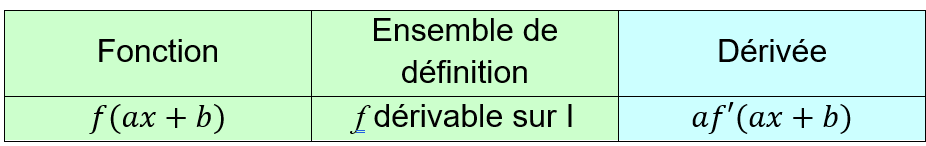
\includegraphics[scale=0.6]{01-06-04}
    \setlength{\arrayrulewidth}{1pt}
    \renewcommand{\arraystretch}{1.9}
    \begin{tabular}{| >{\columncolor{green!25!white}}C{4cm} | >{\columncolor{green!25!white}}C{4cm} | >{\columncolor{cyan!25!white}}C{4cm} | }
    	\hline Fonction & Ensemble de définition& Dérivée  \\
    	\hline$f(ax+b)$ & $f$ dérivable sur I & $af'(ax+b)$ \\
    	\hline
    \end{tabular}
\end{center}
\begin{bmethode}
    $f(x)=\sqrt{5x-4}$\\		
    Alors $f'(x)=5\dfrac{1}{2\sqrt{5x-4}}=\dfrac{5}{2\sqrt{5x-4}}$\\  	 
    En effet : $(5x-4)'=5$ et $(\sqrt{x})'= \dfrac{1}{2\sqrt{x}}$\\ 
\end{bmethode}


\chapter{Probabilités conditionnelles et indépendance}
\thispagestyle{fancy}

\section{Probabilité conditionnelle}

\begin{definition}
    Soit $A$ et $B$ deux événements avec $P(A)\neq 0$.\\
    On appelle probabilité conditionnelle de $B$ sachant $A$, la probabilité que l'événement $B$ se réalise sachant que l'événement $A$ est réalisé. Elle est notée $P_A (B)$  et est définie par : \\$P_A(B)= \dfrac{Card(A \cap B)}{Card(A)}$. 
\end{definition}

\begin{bexemples}
%    \begin{enumEx}
    
%        \item	On tire une carte au hasard dans un jeu de 32 cartes.\\
%        Soit $A$ l'événement \guillemets{Le résultat est un pique}.\\
%        Soit $B$ l'événement \guillemets{Le résultat est un roi}.\\
%        Donc $A \cap B$ est l'événement \guillemets{Le résultat est le roi de pique}.\\
%        
%        Alors : $P(A)= \dfrac{8}{32} = \dfrac{1}{4}$ et $P(A \cap B)= \dfrac{1}{32}$.\\
%        Donc la probabilité que le résultat soit un roi sachant qu'on a tiré un pique est :\\
%        $P_A(B)= \dfrac{Card(A \cap B)}{Card(A)}=\dfrac{\dfrac{1}{32}}{\dfrac{1}{4}}=\dfrac{1}{8}$.\\
%        \ \\
%        On peut retrouver intuitivement ce résultat. En effet, sachant que le résultat est un pique, on a une chance sur 8 d'obtenir le roi.\\
%        \\
%        \item 
        Un sac contient 50 boules, dont 20 boules rouges et 30 boules noires, où il est marqué soit \guillemets{Gagné} ou soit \guillemets{Perdu}.\\ 
        Sur 15 boules rouges, il est marqué Gagné.\\
        Sur 9 boules noires, il est marqué Gagné.\\
        On tire au hasard une boule dans le sac.\\
        Soit $R$ l'événement \guillemets{On tire une boule rouge}.\\
        Soit $G$ l'événement \guillemets{On tire une boule marquée Gagné}.\\
        Donc $R \cap G$ est l'événement \guillemets{On tire une boule rouge marquée Gagné}.\\
        \ \\
        Alors : $P(R)= \dfrac{20}{50} = \dfrac{2}{5}=0,4$ et $P(R \cap G)= \dfrac{15}{50}=\dfrac{3}{10}=0,3$.\\
        Donc la probabilité qu'on tire une boule marquée Gagné sachant qu'elle est rouge est :\\
        $P_R(G)= \dfrac{Card(R \cap G)}{Card(R)}=\dfrac{O,3}{0,4}=\dfrac{3}{4}=0,75$.\\
        \ \\
        On peut retrouver intuitivement ce résultat. En effet, sachant que le résultat est une boule rouge, on a 15 chances sur 20 qu'il soit marqué Gagné.
%    \end{enumEx}
\end{bexemples}

\begin{brmq}
	La probabilité conditionnelle suit les règles et lois de probabilités vues pour les probabilité simples. On a en particulier :
\end{brmq}

\begin{bprop}
    Soit A et B deux événements avec $P(A)\neq 0$.
    \begin{itemProp}
    	\item $0\leq P_A(B)\leq 1$
    	\item $P_A(\overline{B})=1-P_A(B)$
    	\item $P(A \cap B)=P(A)\times P_A (B)$
    \end{itemProp}
\end{bprop}

\section{Arbre pondéré}

\subsection{Exemple}

\begin{bexemple}
    On reprend l'exemple étudié au paragraphe I.
    L'expérience aléatoire peut être schématisée par un arbre pondéré (ou arbre de probabilité) :
%    \begin{center}
%    	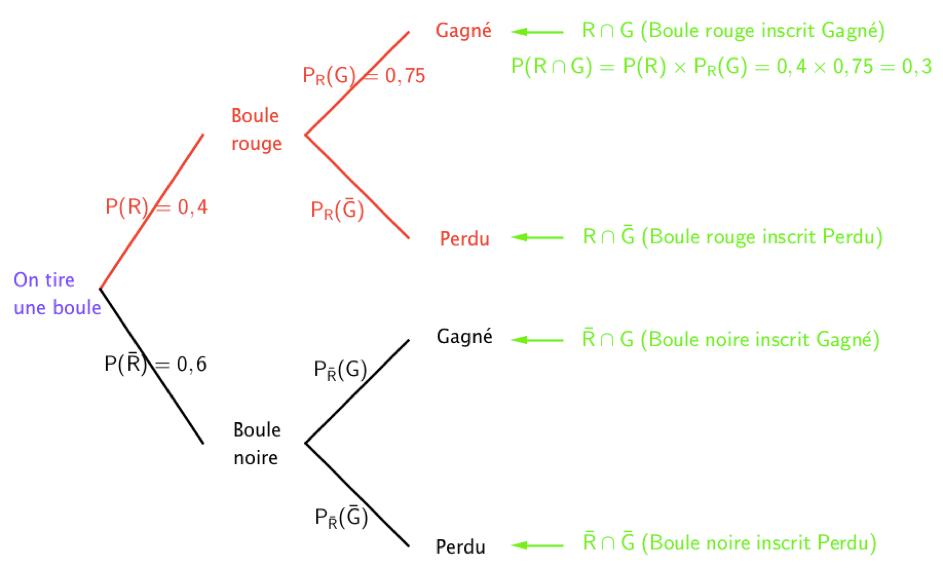
\includegraphics[scale=0.8]{01-09-01.png}
%    \end{center}
	\begin{center}
		%\includegraphics[scale=0.8]{TSTG.04.01.png}\\
		\begin{tikzpicture}[xscale=1,yscale=1]
			% Styles (MODIFIABLES)
			\tikzstyle{fleche}=[->,>=latex,thick]
			\tikzstyle{noeud}=[rectangle]
			\tikzstyle{feuille}=[rectangle]
			\tikzstyle{etiquette}=[midway,fill=white]
			% Dimensions (MODIFIABLES)
			\def\DistanceInterNiveaux{3.8}
			\def\DistanceInterFeuilles{2.5}
			% Dimensions calculées (NON MODIFIABLES)
			\def\NiveauA{(0)*\DistanceInterNiveaux}
			\def\NiveauB{(1.5)*\DistanceInterNiveaux}
			\def\NiveauC{(2.5)*\DistanceInterNiveaux}
			\def\InterFeuilles{(-1)*\DistanceInterFeuilles}
			% Noeuds (MODIFIABLES : Styles et Coefficients d'InterFeuilles)
			\node[noeud] (R) at ({\NiveauA},{(1.5)*\InterFeuilles}) {On tire une boule};
			\node[noeud] (Ra) at ({\NiveauB},{(0.5)*\InterFeuilles}) {Boule Rouge};
			\node[feuille] (Raa) at ({\NiveauC},{(0)*\InterFeuilles}) {Gagné };
			\node[feuille] (Rab) at ({\NiveauC},{(1)*\InterFeuilles}) {Perdu};
			\node[noeud] (Rb) at ({\NiveauB},{(2.5)*\InterFeuilles}) {Boule Noire};
			\node[feuille] (Rba) at ({\NiveauC},{(2)*\InterFeuilles}) {Gagné};
			\node[feuille] (Rbb) at ({\NiveauC},{(3)*\InterFeuilles}) {Perdu};
			% Arcs (MODIFIABLES : Styles)
			\draw[fleche] (R)--(Ra) node[etiquette] {\footnotesize{$P(R)=0,4$}};
			\draw[fleche] (Ra)--(Raa) node[etiquette] {\footnotesize{$P_R(G)=0,75$}};
			\draw[fleche] (Ra)--(Rab) node[etiquette] {\footnotesize{$P_R(\overline{G})$}};
			\draw[fleche] (R)--(Rb) node[etiquette] {\footnotesize{$P(\overline{R})=0,6$}};
			\draw[fleche] (Rb)--(Rba) node[etiquette] {\footnotesize{$P_{\overline{R}}(G)$}};
			\draw[fleche] (Rb)--(Rbb) node[etiquette] {\footnotesize{$P_{\overline{R}}(\overline{G})$}};
			\draw[ForestGreen,<-] (Raa)--($(Raa)+(1.5,0)$) node[right,font=\sffamily] {$R\cap G$ (boule rouge inscrit gagné)} ;
			\draw[white,<-] (Raa)--($(Raa)+(1.5,-0.5)$) node[right,font=\sffamily] {\textcolor{ForestGreen}{$P(R\cap G)=P(R)\times P(G)=0,3$}} ;
			\draw[ForestGreen,<-] (Rab)--($(Rab)+(1.5,0)$) node[right,font=\sffamily] {$R\cap \overline{G}$ (boule rouge inscrit perdu)} ;
			\draw[ForestGreen,<-] (Rba)--($(Rba)+(1.5,0)$) node[right,font=\sffamily] {$\overline{R}\cap G$ (boule noire inscrit gagné)} ;
			\draw[ForestGreen,<-] (Rbb)--($(Rbb)+(1.5,0)$) node[right,font=\sffamily] {$\overline{R}\cap \overline{G}$ (boule noire inscrit perdu)} ;
		\end{tikzpicture}
	\end{center}	
\end{bexemple}
\subsection{Règles}
\begin{bregle}
	La somme des probabilités des branches issues d'un même noeud est égale à 1.
\end{bregle}
\begin{bexemples}
    \begin{itemEx}
        \item A partir du noeud \guillemets{On tire une boule}, on a : $P(R)+P(\overline{R})=0,4+0,6=1$ 
        \item A partir du noeud \guillemets{Boule rouge}, on a : $P_R (\overline{G})=1-P_R(G)=1-0,75=0,25$.	
    \end{itemEx}
\end{bexemples}
Ces exemples font apparaître une formule donnée au paragraphe I.\\

\begin{bregle}
	La probabilité d'une \guillemets{feuille} (extrémité d'un chemin) est égale au produit des probabilités du chemin aboutissant à cette feuille.
\end{bregle}
\begin{bexemple}
	On considère la feuille $R \cap G$.
    On a :\\
     $P(R \cap G)=P(R)\times P_R (G)=0,4\times 0,75=0,3$ 
\end{bexemple}

\begin{bregle}
	\grasInProp{Formule des probabilités totales}\\
	La probabilité d'un événement associé à plusieurs "feuilles" est égale à la somme des probabilités de chacune de ces "feuilles".
\end{bregle}
\begin{bexemple}
    L'événement \guillemets{On tire une boule marquée Gagné} est associé aux feuilles $R \cap G$ et $\overline R \cap G$. On a :\\
    
    $P(R \cap G)=0,3$ et 
    $P(\overline R \cap G)= \dfrac{9}{50} = 0,18$\\ (Probabilité de tirer une boule noire marquée Gagné)\\
    Donc $P(G)=P(R \cap G)+P(\overline R \cap G)=0,3+0,18=0,48$.
\end{bexemple}

%\begin{bmethodet}{Calculer la probabilité d'un événement associé à plusieurs feuilles}
%    Lors d'une épidémie chez des bovins, on s'est aperçu que si la maladie est diagnostiquée suffisamment tôt chez un animal, on peut le guérir ; sinon la maladie est mortelle.\\ 
%    Un test est mis au point et essayé sur un échantillon d'animaux dont 2 \% est porteur de la maladie. On obtient les résultats suivants :\\
%    – si un animal est porteur de la maladie, le test est positif dans 85 \% des cas ;\\
%    – si un animal est sain, le test est négatif dans 95 \% des cas.\\
%    \ \\
%    On choisit de prendre ces fréquences observées comme probabilités pour toute la population et d'utiliser le test pour un dépistage préventif de la maladie.\\
%    \ \\
%    On note respectivement $M$ et $T$ les événements \guillemets{Être porteur de la maladie} et
%    \guillemets{Avoir un test positif}.
%    
%    1) Un animal est choisi au hasard. Quelle est la probabilité que son test soit positif ?\\
%    \emph{D'après BAC S, Antilles-Guyanne 2010}\\	
%    \ \\
%    2) Si le test du bovin est positif, quelle est la probabilité qu'il soit malade ?\\
%    \ \\
%    \ \\
%%    \begin{center}
%%    	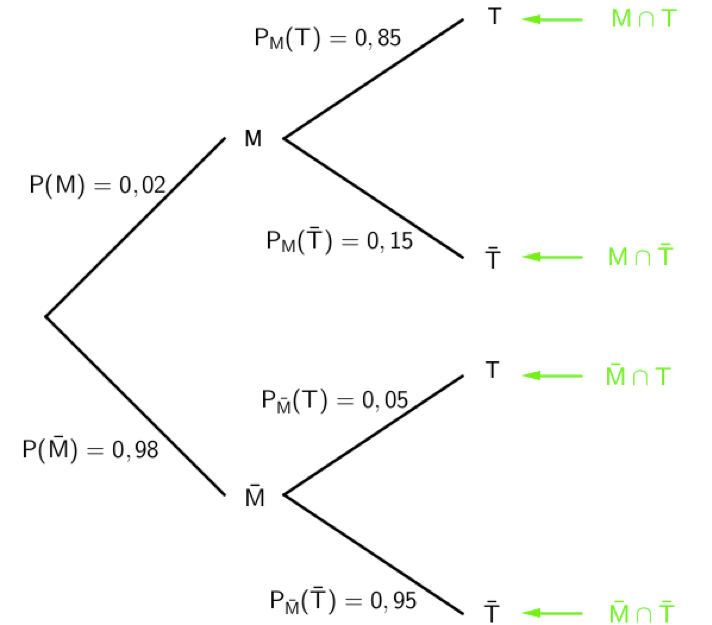
\includegraphics{01-09-02}
%%    \end{center}
%		    \begin{center}
%		%\includegraphics[scale=0.8]{TSTG.04.01.png}\\
%		\begin{tikzpicture}[xscale=1,yscale=1]
%			% Styles (MODIFIABLES)
%			\tikzstyle{fleche}=[->,>=latex,thick]
%			\tikzstyle{noeud}=[rectangle]
%			\tikzstyle{feuille}=[rectangle]
%			\tikzstyle{etiquette}=[midway,fill=white]
%			% Dimensions (MODIFIABLES)
%			\def\DistanceInterNiveaux{4.5}
%			\def\DistanceInterFeuilles{1.5}
%			% Dimensions calculées (NON MODIFIABLES)
%			\def\NiveauA{(0)*\DistanceInterNiveaux}
%			\def\NiveauB{(1.5)*\DistanceInterNiveaux}
%			\def\NiveauC{(2.5)*\DistanceInterNiveaux}
%			\def\InterFeuilles{(-1)*\DistanceInterFeuilles}
%			% Noeuds (MODIFIABLES : Styles et Coefficients d'InterFeuilles)
%			\node[noeud] (R) at ({\NiveauA},{(1.5)*\InterFeuilles}){};
%			\node[noeud] (Ra) at ({\NiveauB},{(0.5)*\InterFeuilles}) {$M$};
%			\node[feuille] (Raa) at ({\NiveauC},{(0)*\InterFeuilles}) {$T$};
%			\node[feuille] (Rab) at ({\NiveauC},{(1)*\InterFeuilles}) {$\overline{T}$};
%			\node[noeud] (Rb) at ({\NiveauB},{(2.5)*\InterFeuilles}) {$\overline{M}$};
%			\node[feuille] (Rba) at ({\NiveauC},{(2)*\InterFeuilles}) {$T$};
%			\node[feuille] (Rbb) at ({\NiveauC},{(3)*\InterFeuilles}) {$\overline{T}$};
%			% Arcs (MODIFIABLES : Styles)
%			\draw[fleche] (R)--(Ra) node[etiquette] {\footnotesize{$P(M)=0,02$}};
%			\draw[fleche] (Ra)--(Raa) node[etiquette] {\footnotesize{$P_M(T)=0,85$}};
%			\draw[fleche] (Ra)--(Rab) node[etiquette] {\footnotesize{$P_M(\overline{T})=0,15$}};
%			\draw[fleche] (R)--(Rb) node[etiquette] {\footnotesize{$P(\overline{M})=0,98$}};
%			\draw[fleche] (Rb)--(Rba) node[etiquette] {\footnotesize{$P_{\overline{M}}(T)=0,05$}};
%			\draw[fleche] (Rb)--(Rbb) node[etiquette] {\footnotesize{$P_{\overline{M}}(\overline{T})=0,95$}};
%			\draw[ForestGreen,<-] (Raa)--($(Raa)+(1.5,0)$) node[right,font=\sffamily] {$M\cap T$} ;
%			%\draw[white,<-] (Raa)--($(Raa)+(1.5,-0.5)$) node[right,font=\sffamily] {\textcolor{ForestGreen}{$P(R\cap G)=P(R)\times P(G)=0,3$}} ;
%			\draw[ForestGreen,<-] (Rab)--($(Rab)+(1.5,0)$) node[right,font=\sffamily] {$M\cap \overline{T}$} ;
%			\draw[ForestGreen,<-] (Rba)--($(Rba)+(1.5,0)$) node[right,font=\sffamily] {$\overline{M}\cap T$} ;
%			\draw[ForestGreen,<-] (Rbb)--($(Rbb)+(1.5,0)$) node[right,font=\sffamily] {$\overline{M}\cap \overline{T}$} ;
%		\end{tikzpicture}
%	\end{center}	
%    La probabilité que le test soit positif est associée aux deux feuilles $M\cap T$ et $\overline M\cap T$.\\
%    $P(T)=P(M\cap T)+P(\overline M\cap T )$ (Formule des probabilités totales)\\
%             $P(T)= 0,02 \times 0,85 + 0,98 \times 0,05 = 0,066$.
%    La probabilité que le test soit positif est égale à 6,6\%. \\
%    \ \\
%    2) $P_T (M)= \dfrac{P(T\cap M)}{P(T)}  = \dfrac{0,02\times 0,85}{0,066} \approx 0,26$.\\
%    La probabilité que le bovin soit malade sachant que le test est positif est d'environ 26\%.
%\end{bmethodet}

\section{Probabilités et indépendance}

\subsection{Indépendance de deux événements}

\begin{bdefi}
	On dit que deux évènements $A$ et $B$ de probabilité non nulle sont indépendants lorsque $P(A\cap B)=P(A)\times P(B)$.
\end{bdefi}

\begin{brmq}
	On a également :
$A$ et $B$ sont indépendants, si et seulement si, $P_A (B)=P(B)$ ou $P_B (A)=P(A)$.
\end{brmq}

\begin{bexemple}
	On tire une carte au hasard dans un jeu de 32 cartes.\\
    Soit $R$ l'événement \guillemets{On tire un roi}.\\
    Soit $T$ l'événement \guillemets{On tire un trèfle}.\\
    Alors $R\cap T$ est l'événement \guillemets{On tire le roi de trèfle}.\\
    \ \\
    On a :\\
    $P(R)  = \dfrac{4}{32} = \dfrac{1}{8}$ , $P(T)= \dfrac{8}{32} = \dfrac{1}{4}$ et $P(R\cap T)= \dfrac{1}{32}$\\ 
    Donc $P(R)\times P(T)  = \dfrac{1}{8} \times \dfrac{1}{4} = \dfrac{1}{32} = P(R\cap T)$\\
    Les événements $R$ et $T$ sont donc indépendants.
    Ainsi, par exemple, $P_T (R)=P(R)$. Ce qui se traduit par la probabilité de tirer un roi parmi les trèfles et égale à la probabilité de tirer un roi parmi toutes les cartes.\\
    \\
    \underline{Contre-exemple :}\\
    On reprend l'expérience précédente en ajoutant deux jokers au jeu de cartes.\\
    Ainsi :
    $P(R)  = \dfrac{4}{34} = \dfrac{2}{17}$, $P(T)= \dfrac{8}{34} = \dfrac{4}{17}$ et $P(R\cap T)= \dfrac{1}{34}$\\
    Donc $P(R)\times P(T)  = \dfrac{2}{17} \times \dfrac{4}{17} = \dfrac{8}{289} \neq P(R\cap T)$\\
    Les événements R et T ne sont donc pas indépendants.
\end{bexemple}

%\begin{bmethodet}{Utiliser l'indépendance de deux événements}
%    Dans une population, un individu est atteint par la maladie $m$ avec une probabilité égale à $0,005$ et par la maladie $n$ avec une probabilité égale à $0,01$.\\
%    On choisit au hasard un individu de cette population.\\
%    Soit $M$ l'événement \guillemets{L'individu a la maladie $m$}.\\
%    Soit $N$ l'événement \guillemets{L'individu a la maladie $n$}.\\
%    On suppose que les événements $M$ et $N$ sont indépendants.\\
%    Calculer la probabilité de l'événement $E$ \guillemets{L'individu a au moins une des deux maladies}.\\
%    \\
%    $P(E)=P(M\cup N)=P(M)+P(N)-P(M\cap N)$\\
%             $P(E)=P(M)+P(N)-P(M)\times P(N)$, car les événements $M$ et $N$ sont indépendants.\\
%             $P(E)= 0,005 + 0,01 – 0,005 \times 0,01 = 0,01495$\\
%    
%    La probabilité qu'un individu choisi au hasard ait au moins une des deux maladies est égale à $0,01495$.\\
%\end{bmethodet}

\begin{bprop}
	Si $A$ et $B$ sont indépendants alors $\overline{A}$ et $B$ sont indépendants.
\end{bprop}

%    \begin{bdemo}
%    $P(\overline{A}\cap B)=P(B\cap \overline{A})$\\
%    $P(\overline{A}\cap B)=P(B)\times P_B (\overline{A})$\\
%    $P(\overline{A}\cap B)=P(B)\times (1-P_B(A))$\\
%    $P(\overline{A}\cap B)=P(B)\times (1-P(A))$ car A et B sont indépendants\\
%    $P(\overline{A}\cap B)=P(B)\times P(\overline{A})$\\
%    \\
%    Donc $\overline{A}$ et $B$ sont indépendants.
%\end{bdemo}

\begin{bexemple}
    Lors d'un week-end prolongé, Bison futé annonce qu'il y a $42\%$ de risque de tomber dans un bouchon sur l'autoroute A6 et $63\%$ sur l'autoroute A7.\\
    Soit $A$ l'événement \guillemets{On tombe dans un bouchon sur l'autoroute A6.}\\
    Soit $B$ l'événement \guillemets{On tombe dans un bouchon sur l'autoroute A7.}\\
    On suppose que les événements $A$ et $B$ sont indépendants.\\
    \\
    Alors les événements $\overline{A}$ et $B$ sont également indépendants et on a :\\
    $P(\overline{A} \cap B)=P(\overline{A})\times P(B)=0,58\times 0,63=0,3654$\\
    \\
    On peut interpréter ce résultat : \\
    La probabilité de tomber dans un bouchon sur l'autoroute A7 mais pas sur l'autoroute A6 est égale à $36,54\%$.
\end{bexemple}

\subsection{Succession de deux épreuves indépendantes}

\begin{bexemples}
    \begin{itemEx}
        \item On lance un dé plusieurs fois de suite et on note à chaque fois le résultat. On répète ainsi la même expérience (lancer un dé) et les expériences sont indépendantes l'une de l'autre (un lancer n'influence pas le résultat d'un autre lancer).
        \item Une urne contient 2 boules blanches et 3 boules noires. On tire au hasard une boule et on la remet dans l'urne.\\
        On répète cette expérience 10 fois de suite. Ces expériences sont identiques et indépendantes.
    \end{itemEx}
\end{bexemples}

\begin{bdefi}
	Plusieurs expériences sont \grasInDef{identiques et indépendantes} si :
    \begin{itemDef}
        \item elles ont les mêmes issues,
        \item chaque issue possède la même probabilité.
    \end{itemDef} 
\end{bdefi}

\begin{bprop}
	On considère une expérience aléatoire à deux issues $A$ et $B$ avec les probabilités $P(A)$ et $P(B)$.\\
    Si on répète l'expérience deux fois de suite :\\
    \begin{itemDef}
        \item la probabilité d'obtenir l'issue $A$ suivie de l'issue $B$ est égale à $P(A) \times P(B)$,
        \item la probabilité d'obtenir l'issue $B$ suivie de l'issue $A$ est égale à $P(B) \times P(A)$,
        \item la probabilité d'obtenir deux fois l'issue $A$ est égale à $P(A)^2$,
        \item la probabilité d'obtenir deux fois l'issue $B$ est égale à $P(B)^2$.
    \end{itemDef}
\end{bprop}

%\begin{bmethodet}{Représenter la répétition d'expériences identiques et indépendantes dans un arbre}
%On considère l'expérience suivante :\\
%Une urne contient 3 boules blanches et 2 boules rouges. On tire au hasard une boule et on la remet dans l'urne. On répète l'expérience deux fois de suite.\\
%1) Représenter l'ensemble des issues de ces expériences dans un arbre.\\
%2) Déterminer la probabilité :\\
%\ \ \ \ \ \ a) d'obtenir deux boules blanches\\
%\ \ \ \ \ \ b) une boule blanche et une boule rouge\\
%\ \ \ \ \ \ c) au moins une boule blanche.\\
%\\
%1) On note $A$ l'issue "On tire une boule blanche" et $B$ l'issue "On tire une boule rouge".
%$P(A) = 3/5 = 0,6$ et $P(B) = 2/5 = 0,4$.\\
%On résume les issues de l'expérience dans un arbre de probabilité :\\
%%\begin{center}
%%	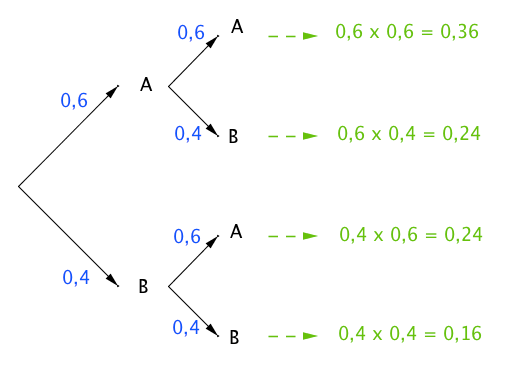
\includegraphics[scale=0.7]{01-09-03}
%%\end{center}
%		    \begin{center}
%	%\includegraphics[scale=0.8]{TSTG.04.01.png}\\
%	\begin{tikzpicture}[xscale=1,yscale=1]
%		% Styles (MODIFIABLES)
%		\tikzstyle{fleche}=[->,>=latex,thick]
%		\tikzstyle{noeud}=[rectangle]
%		\tikzstyle{feuille}=[rectangle]
%		\tikzstyle{etiquette}=[midway,fill=white]
%		% Dimensions (MODIFIABLES)
%		\def\DistanceInterNiveaux{3}
%		\def\DistanceInterFeuilles{1.5}
%		% Dimensions calculées (NON MODIFIABLES)
%		\def\NiveauA{(0)*\DistanceInterNiveaux}
%		\def\NiveauB{(1.5)*\DistanceInterNiveaux}
%		\def\NiveauC{(2.5)*\DistanceInterNiveaux}
%		\def\InterFeuilles{(-1)*\DistanceInterFeuilles}
%		% Noeuds (MODIFIABLES : Styles et Coefficients d'InterFeuilles)
%		\node[noeud] (R) at ({\NiveauA},{(1.5)*\InterFeuilles}){};
%		\node[noeud] (Ra) at ({\NiveauB},{(0.5)*\InterFeuilles}) {$A$};
%		\node[feuille] (Raa) at ({\NiveauC},{(0)*\InterFeuilles}) {$A$};
%		\node[feuille] (Rab) at ({\NiveauC},{(1)*\InterFeuilles}) {$B$};
%		\node[noeud] (Rb) at ({\NiveauB},{(2.5)*\InterFeuilles}) {$B$};
%		\node[feuille] (Rba) at ({\NiveauC},{(2)*\InterFeuilles}) {$A$};
%		\node[feuille] (Rbb) at ({\NiveauC},{(3)*\InterFeuilles}) {$B$};
%		% Arcs (MODIFIABLES : Styles)
%		\draw[fleche] (R)--(Ra) node[etiquette] {\footnotesize{$0,6$}};
%		\draw[fleche] (Ra)--(Raa) node[etiquette] {\footnotesize{$0,6$}};
%		\draw[fleche] (Ra)--(Rab) node[etiquette] {\footnotesize{$0,4$}};
%		\draw[fleche] (R)--(Rb) node[etiquette] {\footnotesize{$0,4$}};
%		\draw[fleche] (Rb)--(Rba) node[etiquette] {\footnotesize{$0,6$}};
%		\draw[fleche] (Rb)--(Rbb) node[etiquette] {\footnotesize{$0,4$}};
%		\draw[ForestGreen,<-] (Raa)--($(Raa)+(1.5,0)$) node[right,font=\sffamily] {$0,6\times 0,6=0,36$} ;
%		%\draw[white,<-] (Raa)--($(Raa)+(1.5,-0.5)$) node[right,font=\sffamily] {\textcolor{ForestGreen}{$P(R\cap G)=P(R)\times P(G)=0,3$}} ;
%		\draw[ForestGreen,<-] (Rab)--($(Rab)+(1.5,0)$) node[right,font=\sffamily] {$0,6\times 0,4=0,24$} ;
%		\draw[ForestGreen,<-] (Rba)--($(Rba)+(1.5,0)$) node[right,font=\sffamily] {$0,4\times 0,6=0,24$} ;
%		\draw[ForestGreen,<-] (Rbb)--($(Rbb)+(1.5,0)$) node[right,font=\sffamily] {$0,4\times 0,4=0,16$} ;
%	\end{tikzpicture}
%\end{center}	
%2)	a) Obtenir deux boules blanches correspond à l'issue $(A ; A)$ :\\
%	$P_1 =  0,36$ (d'après l'arbre).\\
%\\	
%	b) Obtenir une boule blanche et une boule rouge correspond aux issues 
%$(A ; B)$ et $(B ; A)$ :\\
%	$P_2 = 0,24 + 0,24 = 0,48$.\\
%\\
%	b) Obtenir au moins une boule blanche correspond aux issues 
%$(A ; B)$, $(A ; A)$ et $(B ; A)$ :\\
%	$P_3 = 0,24 + 0,36 + 0,24 = 0,84$.
%\end{bmethodet}

\begin{brmq}
    \begin{itemRem}
        \item Pour une expérience dont le nombre d'issues est supérieur à 2, le principe reste le même.
        \item Pour une expérience dont le nombre de répétition est supérieur à 2, le principe reste le même.
    \end{itemRem}
\end{brmq}

\begin{bexemple}
    On lance un dé à six faces 4 fois de suite.\\
    On considère les issues suivantes :\\
    A : On obtient un nombre pair.\\
    B : On obtient un 1.\\
    C : On obtient un 3 ou un 5.\\
    La probabilité d'obtenir la suite d'issues $(A ; B ; A ; C)$ est égale à :\\
    $\dfrac{1}{2}\times \dfrac{1}{6} \times \dfrac{1}{2} \times \dfrac{1}{3}=\dfrac{1}{72}$
\end{bexemple}

\chapter{Suites numériques}
\thispagestyle{fancy}

\begin{bhistoire}
	Dès l'Antiquité, Archimède de Syracuse (-287 ; -212), met en oeuvre une procédure itérative pour trouver une approximation du nombre $\pi$. Il encadre le cercle par des polygones inscrits et circonscrits possédant un nombre de côtés de plus en plus grand. Par ce procédé,
	Archimède donne naissance, sans le savoir, à la notion de suite numérique.\\
	Vers la fin du XVII$^\text{e}$ siècle, des méthodes semblables sont utilisées pour résoudre des équations de façon approchée pour des problèmes de longueurs, d'aires, ...\\
	Un formalisme plus rigoureux de la notion de suite n'apparaitra qu'au début du XIX$^\text{e}$ siècle avec le mathématicien français Augustin Louis Cauchy (1789 ;1857).
\end{bhistoire}


\section{généralités sur les suites numériques}

\subsection{Définition d'une suite numérique}

\begin{bexemplet}{Exemple d'introduction}
	On considère une liste de nombres formée par tous les nombres impairs rangés dans l'ordre croissant : $1,3,5,7, \ldots$\\
	On note $\left(u_{n}\right)$ l'ensemble des éléments de cette suite de nombres tel que :\\
	$u_{0}=1, u_{1}=3, u_{2}=5, u_{3}=7, \ldots$\\
	On a ainsi défini une suite numérique.\\
	On peut lui associer une fonction définie sur $\mathbb{N}$ par 
	$$u: \mathbb{N} \rightarrow \mathbb{R}$$
	$$\phantom{......................}n \mapsto u(n)=u_{n}$$
	
\end{bexemplet}

\begin{bdefi}
	\begin{itemDef}
		\item Une \grasInDef{suite numérique} $\left(u_{n}\right)$ est une liste ordonnée de nombres réels telle qu'à tout entier $n$ on associe un nombre réel noté $u_{n}$.
		\item $u_{n}$ est appelé \grasInDef{le terme de rang $\boldsymbol{n}$} de cette suite (ou d'indice $\left.n\right)$.
	\end{itemDef}
\end{bdefi}

\subsection{Suite définie par une formule explicite}

\begin{bexemples}
	\begin{itemEx}
		\item Pour tout $n$ de $\mathbb{N}$, on donne : $u_{n}=2 n$ qui définit la suite des nombres pairs. Les premiers termes de cette suite sont donc :\\
		$u_{0}=2 \times 0=0$\\
		$u_{1}=2 \times 1=2$\\
		$u_{2}=2 \times 2=4$\\
		$u_{3}=2 \times 3=6$
		\item Pour tout $n$ de $\mathbb{N}$, on donne $: v_{n}=3 n^{2}-1$ Les premiers termes de cette suite sont donc :\\
		$v_{0}=3 \times 0^{2}-1=-1$\\
		$v_{l}=3 \times 1^{2}-1=2$\\
		$v_{2}=3 \times 2^{2}-1=11$\\
		$v_{3}=3 \times 3^{2}-1=26$
	\end{itemEx}
\end{bexemples}
\begin{bdefi}
	Lorsqu'on génère une suite par une formule explicite, chaque terme de la suite est exprimé en fonction de $n$ et indépendamment des termes précédents.
\end{bdefi}

\subsection{Suite définie par une relation de récurrence}
\begin{bexemples}
	\begin{itemEx}
		\item On définit la suite $\left(u_{n}\right)$ par: $u_{0}=5$ et chaque terme de la suite est le triple de son précédent. Les premiers termes de cette suite sont donc :\\
		$u_{0}=5$\\
		$u_{1}=3 \times u_{0}=3 \times 5=15$\\
		$u_{2}=3 \times u_{1}=3 \times 15=45$\\
		De façon générale, on peut noter $: u_{n+1}=3 u_{n}$
		\item On définit la suite $\left(v_{n}\right)$ par : $v_{0}=3$ et pour tout $n$ de $\mathbb{N}, v_{n+1}=4 v_{n}-6$ Les premiers termes de cette suite sont donc :\\
		$v_{0}=3$\\
		$v_{1}=4 v_{0}-6=4 \times 3-6=6$\\
		$v_{2}=4 v_{1}-6=4 \times 6-6=18$\\
		$v_{3}=4 v_{2}-6=4 \times 18-6=66$\\
		Contrairement à une suite définie par une formule explicite, il n'est pas possible, dans l'état, de calculer par exemple $v_{13}$ sans connaître $v_{12}$.\\
		\ \\
		Cependant il est possible d'écrire un algorithme avec Python :
		\begin{center}
			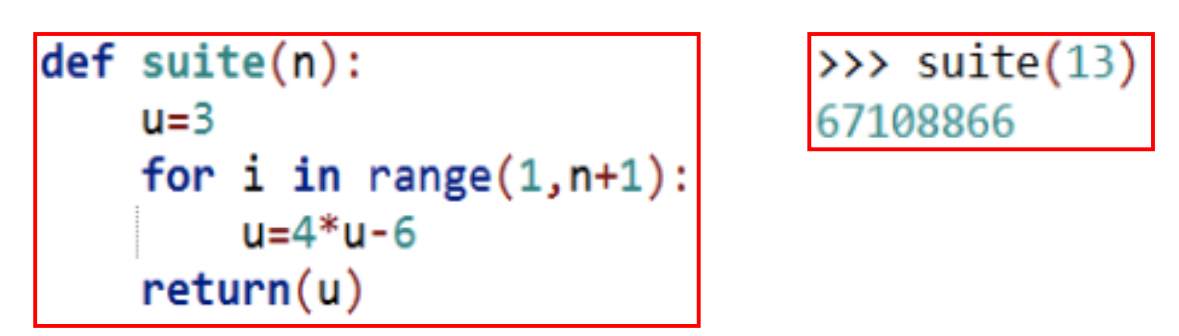
\includegraphics[scale=0.4]{1.08.00-Img01}
		\end{center}
		Ou sur une calculatrice : 
		\begin{center}
			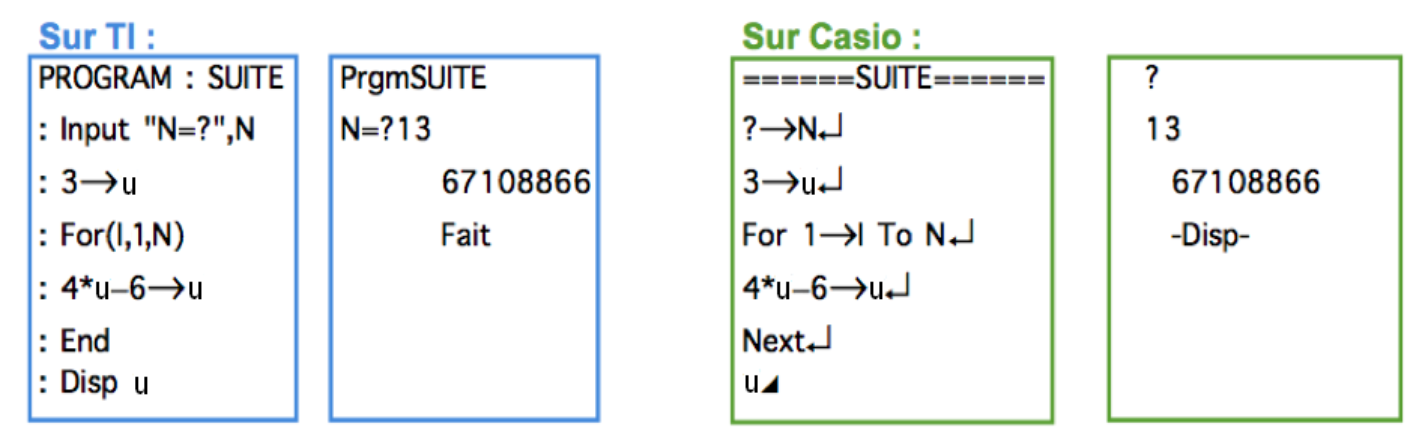
\includegraphics[scale=0.4]{1.08.00-Img02}
		\end{center}
	\end{itemEx}
\end{bexemples}
\begin{bdefi}
	Lorsqu'on génère une suite par une relation de récurrence, chaque terme de la suite s'obtient à partir de son terme précédent.Il faut connaître au moins un terme de la suite pour calculer les autres termes.
\end{bdefi}

\begin{brmq}
	Le mot \emph{récurrence} vient du latin \emph{recurrere} qui signifie "revenir en arrière".
\end{brmq}

\subsection{Représentation graphique d'une suite}

Dans un repère du plan, on représente une suite par un nuage de points de coordonnées $\left(n ; u_{n}\right) .$
\begin{bexemple}
	Pour tout $n$ de $\mathbb{N}$, on donne $: u_{n}=\dfrac{n^{2}}{2}-3$.\\
	On construit le tableau de valeurs avec les premiers termes de la suite :
	\begin{tabular}{|Xc|Xc|Xc|Xc|Xc|Xc|Xc|Xc|Xc|Xc|}
		\hline$n$ & 0 & 1 & 2 & 3 & 4 & 5 & 6 & 7 & 8 \\
		\hline$u_{n}$ & $-3$ & $-2,5$ & $-1$ & 1,5 & 5 & 9,5 & 15 & 21,5 & 29 \\
		\hline
	\end{tabular}\\
	Il est possible d'obtenir un nuage de points à l'aide d'un logiciel.
	\begin{center}
		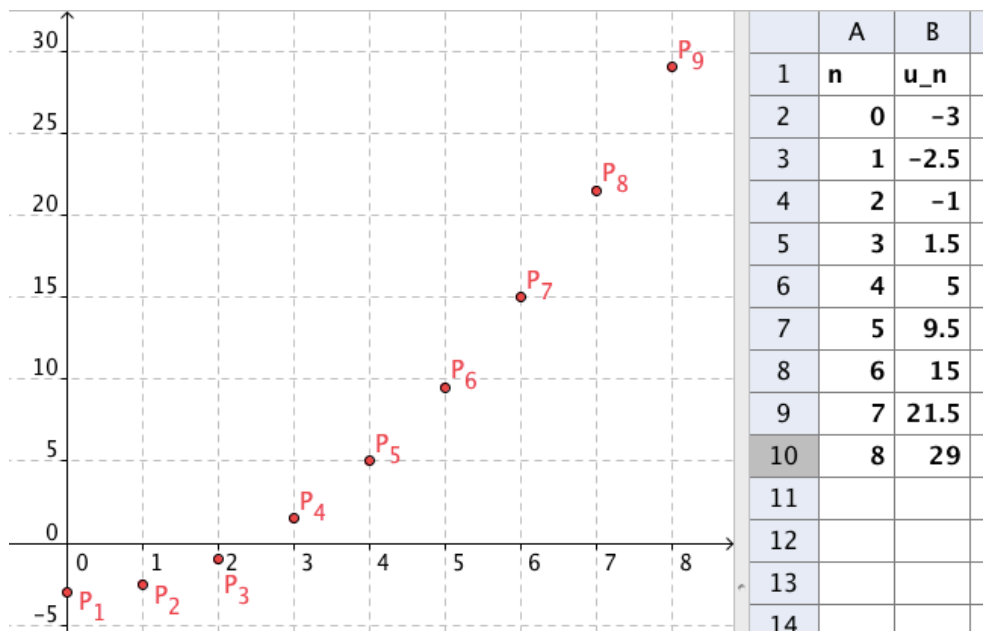
\includegraphics[scale=0.4]{1.08.00-Img03}
	\end{center}
	
\end{bexemple}


\section{Suites arithmétiques}

\subsection{Définition}

\begin{bexemple}
	Considérons une suite numérique $U_n$ où la différence entre un terme et son précédent reste constante et égale à 5.\\
	Si le premier terme est égal à 3, les premiers termes successifs sont :\\
	$U_0 = 3$,\\
	$U_1 = 8$,\\
	$U_2 = 13$,\\
	$U_3 = 18$.\\
	Une telle suite est appelée une suite arithmétique de raison 5 et de premier terme 3.
	La suite est donc définie par : $U_{n+1}=U_n+5$ et $U_0=3$.
\end{bexemple}

\begin{bdefi}
	Une suite $U_n$ est une \grasInDef{suite arithmétique} s'il existe un nombre r tel que pour tout entier $n$, on a : $U_{n+1}=U_n+r$.
	Le nombre $r$ est appelé \grasInDef{raison} de la suite.
\end{bdefi}
\ \\
\begin{bmethodet}{Démontrer si une suite est arithmétique}
	1) La suite $U_n$ définie par : $U_n=7-9n$ est-elle arithmétique ?\\
	2) La suite $V_n$ définie par : $V_n=n^2+3$ est-elle arithmétique ?\\
	\\
	1) $U_{n+1}-U_n=7-9(n+1)-7+9n=7-9n-9-7+9n=-9$.\\
	La différence entre un terme et son précédent reste constante et égale à –9.\\
	$U_n$ est une suite arithmétique de raison $–9$.\\
	
	2) $V_{n+1}-V_n=(n+1)^2+3-n^2-3=n^2+2n+1+3-n^2-3=2n+1$.\\
	La différence entre un terme et son précédent ne reste pas constante.\\
	$V_n$ n'est pas une suite arithmétique.
\end{bmethodet}

\begin{bprop}
	$U_n$ est une suite arithmétique de raison $r$ et de premier terme $U_0$.\\
	Pour tout entier naturel $n$, on a : $U_n=U_0+nr$.
\end{bprop}

\begin{bdemo}
	La suite arithmétique $U_n$ de raison $r$ et de premier terme $U_0$ vérifie la relation $U_{n+1}=U_n+r$.\\
	En calculant les premiers termes :\\
	$U_1=u_0+r$\\ 
	$U_2=u_1+r$\\
	$U_3=u_2+r$\\
	…\\
	$U_n=U_{n-1}+r$\\
	
	En additionnant membre à membre ces n égalités, on obtient :\\
	$U_1+U_2+U_3+...+U_n=U_0+U_1+U_2+...+U_{n-1}+n\times r$\\
	Soit, en retranchant aux deux membres les termes identiques :
	$U_n=U_0+nr$
\end{bdemo}

\begin{bmethodet}{Déterminer la raison et le premier terme d'une suite arithmétique}
	Considérons la suite arithmétique $U_n$ tel que $U_5=7$ et $U_9=19$.\\
	1) Déterminer la raison et le premier terme de la suite $U_n$.\\
	2) Exprimer $U_n$ en fonction de $n$.\\ 
	\\
	1) Les termes de la suite sont de la forme $U_n=U_0+nr$\\
	Ainsi 	$U_5=U_0+5r=7$  et $U_9=U_0+9r=19$.\\
	En soustrayant membre à membre, on obtient :\\ $U_0+5r-U_0-9r=7-19$\\
	Soit : $5r-9r=7-19$ donc $r=3$.
	
	Comme $U_0+5r=7$, on a : $U_0+5\times 3=7$ et donc : $U_0=-8$.\\
	\\
	2) $U_n=U_0+nr$  soit  $U_n=-8+n\times 3$ ou encore $U_n=3n-8$
\end{bmethodet}

\subsection{Représentation graphique}

Les points de la représentation graphique d'une suite arithmétique sont alignés.

\begin{bexemple}
	On a représenté ci-dessous la suite de raison $–0,5$ et de premier terme $4$.
	\begin{center}
		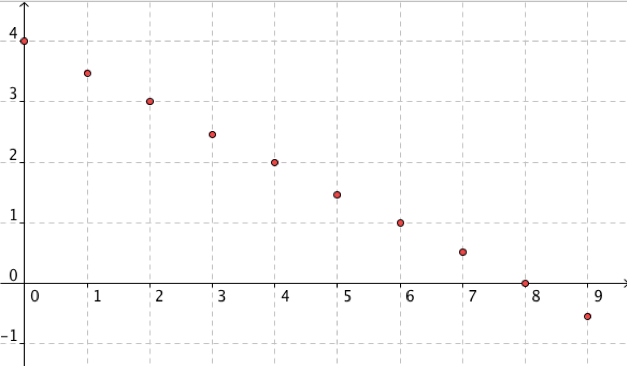
\includegraphics[scale=1]{01-07-01}
	\end{center}
\end{bexemple}

\section{Somme des termes consécutifs: suite arithmétique}

\begin{bprop}
	$n$ est un entier naturel non nul alors on a : $1+2+3+...+n= \dfrac{n(n+1)}{2}$
\end{bprop}

\begin{brmq}
	Il s'agit de la somme des $n$ premiers termes d'une suite arithmétique de raison $1$ et de premier terme $1$
\end{brmq}

\begin{bdemo}
	\begin{tabular}{ c c c c c c c c c c c c }			
		& 1 & + & 2 & + & 3 & + &... & + &n-1 & + & n \\
		+ & n & + & n-1 & + & n-2 & + & ...& + & 2 & + & 1 \\
		\hline
		& (n+1) & + & (n+1) & + & (n+1) & + & ... & + & (n+1) & + & (n+1)\\
	\end{tabular} \\
	\\
	Donc : $2\times (1+2+3+...+(n-1)+n)=n(n+1)$\\
	Et donc : $1+2+3+...+(n-1)+n=\dfrac{n(n+1)}{2}$
\end{bdemo}

\begin{bmethodet}{Calculer la somme des termes d'une suite arithmétique}
	Calculer les sommes $S_1$ et $S_2$ suivantes :\\ 
	$S_1=1+2+3+...+348$\ \ \ \ \ \ \ \ \ \ \ \ \ \ \ \ \ \ \ \ \ \ \ $S_2=33+36+39+...+267$
	\\
	\\
	$S_1=1+2+3+...+348=\dfrac{348\times 349}{2}=60726$\\
	\\
	\\
	$S_2=33+36+39+...+267=3\times(11+12+13+...+89)$\\
	$=3\times((1+2+3+...+89)-(1+2+3+...+10))$\\
	$=3\times \left(\dfrac{89\times 90}{2}-\dfrac{10\times11}{2}\right)=11\ 850$
\end{bmethodet}

\section{Suites géométriques}

\subsection{Définition}

\begin{bexemple}
	Considérons une suite numérique $U_n$ où le rapport entre un terme et son précédent reste constant et égale à 2.\\
	Si le premier terme est égal à 5, les premiers termes successifs sont :\\
	$U_0 = 5$,\ \ \ 
	$U_1 = 10$,\ \ \ 
	$U_2 = 20$,\ \ \ 
	$U_3 = 40$.\\
	Une telle suite est appelée une suite géométrique de raison $2$ et de premier terme $5$.\\
	La suite est donc définie par : $U_{n+1}=2\times U_n$ et $U_0=5$. 
\end{bexemple}

\begin{bdefi}
	Une suite $U_n$ est une \grasInDef{suite géométrique} s'il existe un nombre q tel que pour tout entier $n$, on a : $U_{n+1}=q\times U_n$.
	Le nombre $q$ est appelé \grasInDef{raison} de la suite.
\end{bdefi}

\begin{bmethodet}{Démontrer si une suite est géométrique}
	La suite $U_n$ définie par : $U_n=3\times 5^n$  est-elle géométrique ?
	\ \\
	$\dfrac{U_{n+1}}{U_n} =\dfrac{3\times 5^{n+1}}{3\times 5^n}=\dfrac{5^{n+1}}{5^n} =5^{n+1-n}=5$\\
	Le rapport entre un terme et son précédent reste constant et égale à $5$.\\
	$U_n$ est une suite géométrique de raison $5$ et de premier terme $U_0=3\times 5^0=3$.
\end{bmethodet}

\begin{bexemplet}{exemple concret}
	On place un capital de \EUR{500} sur un compte dont les intérêts annuels s'élèvent à $4\%$.
	Chaque année, le capital est multiplié par $1,04$.
	Ce capital suit une progression géométrique de raison $1,04$.\\
	
	On a ainsi :\\ 
	$U_1=1,04\times 500=520$\\		
	$U_2=1,04\times 520=540,80$\\
	$U_3=1,04\times 540,80=562,432$\\	
	De manière générale : $U_{n+1}=1,04\times U_n$ avec $U_0=500$\\ 
	On peut également exprimer $U_n$ en fonction de $n$ : $U_n= 500\times1,04^n$. 
\end{bexemplet}

\begin{propriete}
	$U_n$ est une suite géométrique de raison $q$ et de premier terme $U_0$.\\
	Pour tout entier naturel $n$, on a : $U_n= U_0\times q^n$.
\end{propriete}

\begin{bdemo}
	La suite géométrique $U_n$ de raison $q$ et de premier terme $U_0$ vérifie la relation
	$U_{n+1}=q\times U_n$.
	\begin{itemDem}
		\item Si $q$ ou $U_0$ est nul, alors tous les termes de la suite sont nuls. La démonstration est évidente dans ce cas.
		\item Dans la suite, on suppose donc que $q$ et $U_0$ sont non nuls. Dans ce cas, tous les termes de la suite sont non nuls.
	\end{itemDem}
	En calculant les premiers termes :\\ 
	$U_1=q\times U_0$\\
	$U_2=q\times U_1$\\
	$U_3=q\times U_2$\\
	…\\
	$U_n=q\times U_{n-1}$\\
	\\
	En multipliant membre à membre ces $n$ égalités, on obtient :
	$u_1\times U_2\times U_3\times …\times U_n=U_0\times U_1\times U_2\times …\times u_{n-1}\times q^n$.\\
	Comme les termes de la suite sont non nuls, on peut diviser aux deux membres les facteurs identiques : $U_n=U_0\times q^n$
\end{bdemo}

\begin{bmethodet}{Déterminer la raison et le premier terme d'une suite géométrique}
	Considérons la suite géométrique $U_n$ tel que $U_4=8$ et $U_7=512$.\\
	Déterminer la raison et le premier terme de la suite $U_n$.\\
	\\
	\ \\
	Les termes de la suite sont de la forme $U_n=U_0\times q^n$.\\
	Donc : $U_4=U_0\times q^4=8$ et $U_7=U_0\times q^7=512$.\\
	Ainsi : $\dfrac{U_7}{U_4}  = \dfrac{U_0\times q^7}{U_0\times q^4}  =q^3$ et $\dfrac{U_7}{U_4}=\dfrac{512}{8}=64$ donc $q^3=64$.\\
	On utilise la fonction racine troisième de la calculatrice pour trouver le nombre qui élevé au cube donne 64.\\
	Ainsi $q=^3\sqrt{64}=4$\\
	Comme $U_0 \times q^4=8$, on a : $U_0\times 4^4=8$ et donc : $U_0= \dfrac{1}{32}$.
\end{bmethodet}

\subsection{Représentation graphique}

\begin{bexemple}
	La suite géométrique $U_n$ définie par $U_n=-4\times2^n$ est décroissante car le premier terme est négatif et la raison est supérieure à 1
	\begin{center}
		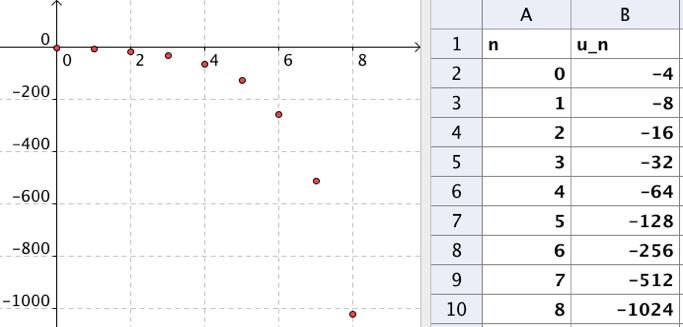
\includegraphics[scale=1]{01-07-03.png}
	\end{center}
	Remarque : Si la raison q est négative alors la suite géométrique n'est pas monotone.
\end{bexemple}
% \begin{center}
	%     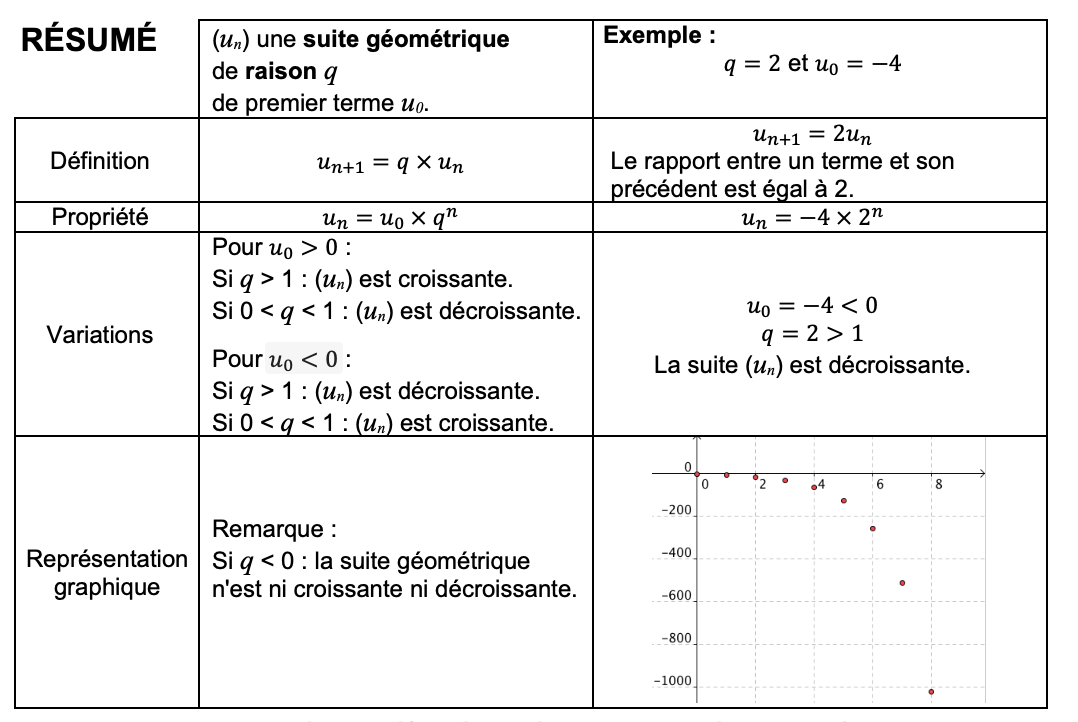
\includegraphics[scale=0.8]{01-07-04.png}
	% \end{center}

\section{Somme des termes consécutifs d'une suite géométrique}

\begin{bprop}
	$n$ est un entier naturel non nul et $q$ un réel différent de 1 alors on a :\\ 
	$1+q+q^2+q^3+...+q^n= \dfrac{1-q^{n+1}}{1-q}$
\end{bprop}

\begin{brmq}
	Il s'agit de la somme des $n+1$ premiers termes d'une suite géométrique de raison $q$ et de premier terme $1$.
\end{brmq}

\begin{bdemo}
	$S=1+q+q^2+q^3+...+q^n$\\
	$q\times S=q+q^2+q^3+q^4+...+q^(n+1)$\\
	\\
	Ainsi :\\
	$S-q\times S=(1+q+q^2+q^3+...+q^n )-(q+q^2+q^3+q^4+...+q^{n+1})$\\
	$S-q\times S=1-q^(n+1)$\\
	$S\times (1-q)=1-q^{n+1}$\\
	$S=\dfrac{1-q^(n+1)}{1-q}$
\end{bdemo}

\begin{bmethodet}{Calculer la somme des termes d'une suite arithmétique}
	Calculer la somme $S$ suivante : 
	$S=1+3+3^2+3^3+...+3^{13}$\\
	\\
	$S=1+3+3^2+3^3+...+3^{13}=\dfrac{1-3^{14}}{1-3}=2\  391\  484$
	
\end{bmethodet}





\chapter{Fonction exponentielle}
\thispagestyle{fancy}

\section{Définition de la fonction exponentielle}

    \begin{bdefi}
        Il existe une unique fonction $f$ dérivable sur \R telle que $f'=f$  et $f(0)=1$. Cette fonction s'appelle \grasInDef{fonction exponentielle} et se note \grasInDef{exp}.
    \end{bdefi}

    \begin{bcscq}
        $\exp(0)=1$
    \end{bcscq}
    
    Avec la calculatrice, il est possible d'observer l'allure de la courbe représentative de la fonction exponentielle :
    \begin{center}
        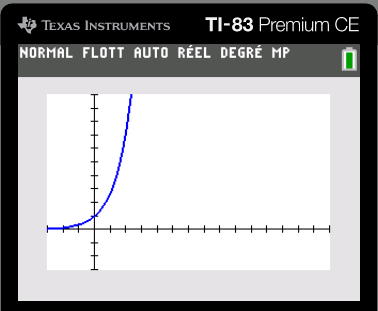
\includegraphics[scale=0.6]{01-12-01}
    \end{center}
    
    \begin{bprop}
        La fonction exponentielle est strictement positive sur \R.
    \end{bprop}
    
\section{Étude de la fonction exponentielle}

    \subsection{Dérivabilité}
    
        \begin{bprop}
            La fonction exponentielle est dérivable sur \R et $(\exp(x))'=\exp(x)$
        \end{bprop}
    \subsection{Variations}
        \begin{bprop}
            La fonction exponentielle est strictement croissante sur \R.
        \end{bprop}
        
        En effet, $(\exp(x))'>0$ car $(\exp(x))'=\exp(x)>0$.
        
    \subsection{Courbe représentative}
    
        On dresse le tableau de variations de la fonction exponentielle :
        
        \begin{multicols}{2}
            \begin{center}
                \begin{tikzpicture}
                    \tkzTabInit{$x$ / 0.8 , $(\exp(x))'$ / 0.8, $\exp(x)$ / 1.2}{$-\infty$, $+\infty$}
                    \tkzTabLine{, +,  }
                    \tkzTabVar{-/ $0$ ,  +/ $+\infty$}
                \end{tikzpicture}
            \end{center}
            
            \begin{center}
                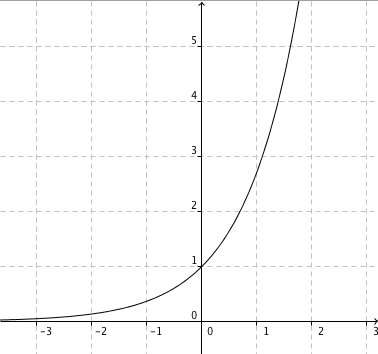
\includegraphics[scale=0.6]{01-12-02}
            \end{center}
        \end{multicols}
        
\section{Propriété de la fonction exponentielle}

    \subsection{relation fonctionnelle}
    
        \begin{bthm}
            Pour tous réels $x$ et $y$, on a : $\exp(x+y)=\exp(x)\times \exp(y)$
        \end{bthm}
        
        \begin{brmq}
            Cette formule permet de transformer une somme en produit et réciproquement.
        \end{brmq}
        
        \begin{bcor}
            Pour tous réels $x$ et $y$, on a :
            \begin{itemDef}
                \item $\exp(-x)=\dfrac{1}{\exp(x)}$ ou encore $\exp(x)\times\exp(-x)=1$
                \item $\exp(x-y)=\dfrac{\exp(x)}{\exp(y)}$
                \item $\exp(nx) = \exp(x)^n$ avec $n \in \N$
            \end{itemDef}
        \end{bcor}
        
        \begin{bdemot}{Démonstration du a et b}
            \begin{itemMet}
                \item $\exp(x)\times\exp(-x)=\exp(x-x)=\exp(0)=1$
                \item $\exp(x-y)=\exp(x+(-y))=\exp(x)\times\exp(-y)=\exp(x)\times\dfrac{1}{\exp(y)}=\dfrac{\exp(x)}{\exp(y)}$
            \end{itemMet}
        \end{bdemot}
        
    \subsection{Le nombre e}
    
        \begin{bdefi}
            L'image de $1$ par la fonction exponentielle est notée $\e$.\\
            On a ainsi $\exp(1) = \e$
        \end{bdefi}
        
        \begin{brmq}
            Avec la calculatrice, on peut obtenir une valeur approchée de $\e$.
            \begin{center}
                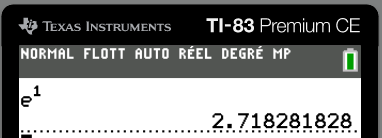
\includegraphics[scale=0.7]{01-12-03}
            \end{center}
        \end{brmq}
        
        \begin{bnota}
            $\exp(x)=\exp(1\times x)=(\exp(1))^x=\e^x$\\
            On note pour tout $x$ réel, $\exp(x)=\e^x$
        \end{bnota}
        
        Avec cette nouvelle notation, on peut ainsi résumer l'ensemble des propriétés de la fonction exponentielle :
        
        \begin{bprops}
            Pour tous réels $x$ et $y$, on a :
            \begin{enumDef}
                \item $\e^0=1$ et $\e^1=e$
                \item $\e^x>0$ et $(\e^x)'=\e^x$
                \item $\e^{x+y}=\e^x\times\e^y\ \ \ \ \ \ \ \ \ \ \ \ \e^{x-y}=\dfrac{\e^x}{\e^y}\ \ \ \ \ \ \ \ \ \ \ \ \e^{-x}=\dfrac{1}{\e^{x}}\ \ \ \ \ \ \ \ \ \ \ \ (\e^x)^n=\e^{nx}$, avec $n \in \N$
                \item $(\e^{ax+b})'=a\e^{ax+b}$
            \end{enumDef}
        \end{bprops}
        \begin{bmethodet}{Dériver une fonction exponentielle}
            \grasInMet{Enoncé :} Dériver les fonctions suivantes.
            \begin{enumMet}
                \begin{multicols}{2}
                    \item $f(x)=4x-3\e^x$
                    \item $g(x)=(x-1)\e^x$
                    \item $h(x)=\dfrac{e^x}{x}$
                    \item $j(x)=\e^{3x+2}$
                \end{multicols}
            \end{enumMet}
            \grasInMet{Réponse :}
            \begin{enumMet}
                \begin{multicols}{2}
                    \item $f'(x)=4-3\e^x$
                    \item $g'(x)=1\times \e^x + (x-1)\e^x=\e^x+x\e^x-\e^x=x\e^x$
                    \item $h'(x)=\dfrac{e^x\times x-\e^x\times 1}{x^2}=\dfrac{\e^x(x-1)}{x^2}$
                    \item $j'(x)=3\e^{3x+2}$
                \end{multicols}
            \end{enumMet}
        \end{bmethodet}
        \begin{bmethodet}{Simplifier les écritures}
            \grasInMet{Enoncé :} Simplifier l'écriture des nombres suivants.
            \begin{enumMet}
                \begin{multicols}{2}
                    \item $A=\dfrac{\e^7\times\e^{-4}}{\e^{-5}}$
                    \item $B=(\e^5)^{-6}\times \e^{-3}$
                    \item $C=\dfrac{1}{(\e^{-3})^2}+\dfrac{(\e^4)^{-1}}{\e^2\times\e^{-6}}$
                    \item $D=\dfrac{(\e^{2x})^3}{\e^{3x+1}\times \e^{-x-1}}$
                \end{multicols}
            \end{enumMet}
            \grasInMet{Réponse :}
            \begin{enumMet}
                \item $A=\dfrac{\e^7\times\e^{-4}}{\e^{-5}}=\dfrac{\e^{7-4}}{\e^{-5}}=\dfrac{\e^{3}}{\e^{-5}}=\e^{3-(-5)}=\e^8$
                \item $B=(\e^5)^{-6}\times \e^{-3}=\e^{5\times(-6)}\times \e^{-3}=\e^{-30}\times \e^{-3}=\e^{-30-3}=\e^{-33}$
                \item $C=\dfrac{1}{(\e^{-3})^2}+\dfrac{(\e^4)^{-1}}{\e^2\times\e^{-6}}=\dfrac{1}{\e^{-3\times2}}+\dfrac{\e^{4\times(-1)}}{\e^{2-6}}=\dfrac{1}{\e^{-6}}+\dfrac{\e^{-4}}{\e^{-4}}=\e^6+1$
                \item $D=\dfrac{(\e^{2x})^3}{\e^{3x+1}\times \e^{-x-1}}=\dfrac{\e^{2x \times 3}}{\e^{3x+1-x-1}}=\dfrac{\e^{6x}}{\e^{2x}}=\e^{6x-2x}=\e^{4x}$
            \end{enumMet}
        \end{bmethodet}
        \begin{bprops}
            Pour tous réels $a$ et $b$, on a :
            \begin{itemDef}
                \item $\e^a=\e^b \iff a=b$
                \item $\e^a<\e^b \iff a<b$
            \end{itemDef}
        \end{bprops}
        \begin{bmethodet}{Résoudre une équation ou une inéquation}
            \grasInMet{Enoncé :}
            \begin{enumMet}
                \item Résoudre dans \R l'équation $\e^{x^2-3}-\e^{-2x}=0$.
                \item Résoudre dans \R l'inéquation $\e^{4x-1}\ge 1$.
            \end{enumMet}
            \grasInMet{Réponse :}
            \begin{enumMet}
                \item $\e^{x^2-3}-\e^{-2x}=0 \iff \e^{x^2-3}=\e^{-2x} \iff x^2-3=-2x \iff x^2+2x-3=0$\\
                $\Delta=2^2-4\times1\times(-3)=16$\\
                Donc $x_1=\dfrac{-2-\sqrt{16}}{2\times1}=-3$ ou $x_2=\dfrac{-2+\sqrt{16}}{2\times1}=1$\\
                Les solutions sont $–3$ et $1$.
                \item $\e^{4x-1}\ge 1 \iff \e^{4x-1}\ge \e^0 \iff 4x-1\ge 0 \iff x\ge \dfrac{1}{4}$\\
                L'ensemble des solutions est l'intervalle $\intervFO{\dfrac{1}{4}}{+\infty}$.
            \end{enumMet}
        \end{bmethodet}
        \begin{bmethodet}{Étudier une fonction exponentielle}
            \grasInMet{Enoncé :} Soit $f$ la fonction définie sur \R par $f(x)=(x+1) \e^x$.
            \begin{enumMet}
                \item Calculer la dérivée de la fonction $f$.
                \item Dresser le tableau de variations de la fonction $f$.
                \item Déterminer une équation de la tangente à la courbe au point d'abscisse 0.
                \item Tracer la courbe représentative de la fonction $f$ en s'aidant de la calculatrice.
            \end{enumMet}
            \grasInMet{Réponse :}
            \begin{enumMet}
                \item $f'(x)=\e^x+(x+1)\e^x=(x+2)\e^x$\\
                \item Comme $e^x>0$, $f'(x)$ est du signe de $x+2$.\\
                $f$ est donc décroissante sur l'intervalle $\intervOF{-\infty}{-2}$ et croissante sur l'intervalle $\intervFO{-2}{+\infty}$.\\
                On dresse le tableau de variations :\\
                \begin{center}
                    \begin{tikzpicture}
                        \tkzTabInit{$x$ / 1 , $f'(x)$ / 1, $f(x)$ / 1.5}{$-\infty$, $-2$, $+\infty$}
                        \tkzTabLine{, -, z, +, }
                        \tkzTabVar{+/  , -/ $-e^{-2}$, +/ }
                    \end{tikzpicture}
                \end{center}
                \item $f(0)=1$  et $f'(0)=2$\\
                Une équation de la tangente à la courbe en 0 est donc : $y=f'(0)(x-0)+f(0)$, soit : $y=2x+1$
                \item \ \\
                \begin{center}
                    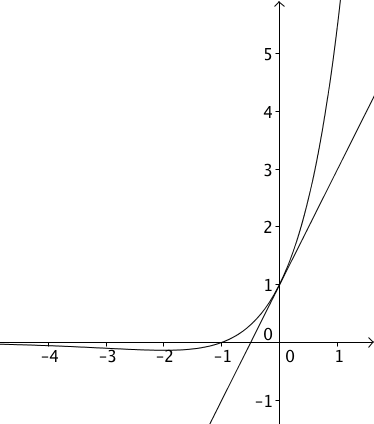
\includegraphics[scale=0.6]{01-12-04}
                \end{center}
            \end{enumMet}
        \end{bmethodet}
    % \section{Exponentielle et suite géométrique}
    %     On a vu que pour tout entier $n$, et tout réel $a$, on a : $e^{na}=(e^a )^n$, ainsi :
        
    %     \begin{propriete}
    %         La suite $(e^{na})$ est une suite géométrique de raison $e^a$.
    %     \end{propriete}

    %     On rappelle qu'une suite géométrique de raison $q$ et de premier terme $u_0$ a pour terme général : $u_n=u_0 q^n$. 
        
    %     \begin{methodeTitre}{Déterminer une suite géométrique comprenant une exponentielle}
    %         \grasInMet{Enoncé :} \\
    %         1) Dans chaque cas, déterminer la raison et le premier terme de la suite géométrique dont le terme général est :\\
    %         a) $u_n=e^{4n}$\hspace{2cm} b) $u_n=2e^{-3n}$\hspace{2cm} c) $u_n=-e^{\dfrac{n}{3}}$\hspace{2cm} d) $u_n=e^{2n-1}$\\
    %         \ \\
    %         2) Déterminer le terme général d'une suite géométrique de raison $\dfrac{1}{e}$ et de premier terme $3$.
    %         \grasInMet{Réponse :}
    %         1) a) $u_n=e^4n=1(e^4)^n$\\ 
    %         $(u_n )$ est une suite géométrique de raison $e^4$ et de premier terme $1$.\\
    %         \ \\
    %         b) $u_n=2e^{-3n}=2(e^{-3})^n$\\ 
    %         $(u_n )$ est une suite géométrique de raison $e^{-3}$ et de premier terme $2$.\\
    %         \ \\
    %         c) $u_n=-e^{\frac{n}{3}}=(-1)(e^{\frac{1}{3}})^n$\\
    %         $(u_n )$ est une suite géométrique de raison $e^{\frac{1}{3}}$ et de premier terme $–1$.\\
    %         \ \\
    %         d) $u_n=e^{2n-1}=e^{2n}\times e^{-1}=e^{-1}\times(e^2)^n= \dfrac{1}{e}\times(e^2)^n$\\
    %         $(u_n )$ est une suite géométrique de raison $e^2$ et de premier terme $\dfrac{1}{e}$.\\
    %         \ \\
    %         2) $(u_n )$ est suite géométrique de raison $\dfrac{1}{e}$ et de premier terme 3, donc :\\
    %         $u_n=3\times\dfrac{1}{e}^n=3(e^{-1})^n=3e^{-n}$.
    %     \end{methodeTitre}
        
    \section{Fonctions de la forme $t\mapsto e^{kt}$}
        \subsection{variations}
            \begin{bprop}
                La fonction $t\mapsto e^{kt}$ avec $k\in \R\textbackslash \{0 \}$, est dérivable sur \R. Sa dérivée est la fonction  $t\mapsto ke^{kt}$
            \end{bprop}
            
            \begin{bdemo}
                On rappelle que la dérivée d'une fonction composée $t\mapsto g(at+b)$ est $t\mapsto ag'(at+b)$
                En considérant $g(t)=e^t$, $a=k$ et $b=0$, on a : $(e^{kt})'=ke^{kt}$.
            \end{bdemo}
            
            \begin{bexemple}
                Soit $f(t)=e^{-4t}$ alors $f'(t)=-4e^{-4t}$.
            \end{bexemple}
            
            \begin{bprop}
                \begin{itemDef}
                    \item Si $k > 0$ : la fonction $t\mapsto e^{kt}$ est croissante.
                    \item Si $k < 0$ : la fonction $t\mapsto e^{kt}$ est décroissante.
                \end{itemDef}
            \end{bprop}
            
            \begin{bdemo}
                On a : $(e^{kt} )'=ke^{kt}$\\
                Or, $e^{kt}>0$ pour tout réel $t$ et tout entier relatif $k$ non nul.\\
                Donc le signe de la dérivée $t\mapsto ke^{kt}$dépend du signe de $k$.\\
                \begin{itemDem}
                \item Si $k > 0$ alors la dérivée est positive est donc la fonction $t\mapsto e^{kt}$ est croissante.
                \item Si $k < 0$ alors la dérivée est négative est donc la fonction $t\mapsto e^{kt}$ est décroissante.\\
                \end{itemDem}
            \end{bdemo}
            
        \subsection{Représentation graphique}
        
            \begin{center}
                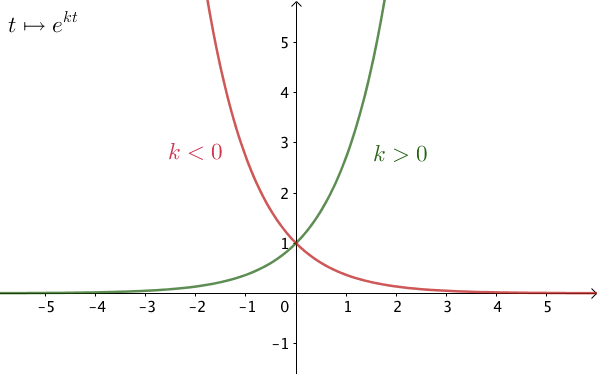
\includegraphics[scale=0.5]{01-12-05}
            \end{center}
            
            \begin{bmethodet}{Étudier une fonction $t\mapsto e^{kt}$ dans une situation concrète }
                \grasInMet{Enoncé :} \\
                Suite à une infection, le nombre de bactéries contenues dans un organisme en fonction du temps (en heures) peut être modélisé par la fonction $f$ définie sur $[0 ; 10]$ 
                et telle que $f'(t)=0,14f(t)$.
                \begin{enumMet}
                    \item Montrer que la fonction $f$ définie sur $[0 ; 10]$ par $f(t)=Ae^{0,14t}$ convient.
                    \item On suppose que $f(0)=50000$. Déterminer $A$.
                    \item Déterminer les variations de $f$ sur $[0 ; 10]$.
                    \item  \begin{enumMet}
                        \item À l'aide de la calculatrice, donner un arrondi au millier près du nombre de bactéries après 3h puis 5h30.
                        \item À l'aide de la calculatrice, déterminer au bout de combien de temps le nombre de bactéries a-t-il doublé. Arrondir à l'heure près.
                    \end{enumMet}
                \end{enumMet}
                \grasInMet{Réponse :}
                \begin{enumMet}
                    \item $f'(t)=A\times 0,14e^{0,14t}=0,14\times Ae^{0,14t}=0,14f(t)$.\\
                La fonction $f$ définie sur $[0 ; 10]$ par $f(t)=Ae^{0,14t}$ vérifie bien l'égalité
                $f'(t)=0,14f(t)$ donc elle convient.
                    \item $f(0)=Ae^{0,14\times0}=Ae^0=A$.\\
                Donc, si $f(0)=50000$, on a : $A=50000$.\\
                Une expression de la fonction $f$ est donc : $f(t)=50000e^{0,14t}$.
                    \item Comme $k=0,14>0$, on en déduit que la fonction $t\mapsto e^{0,14t}$ est strictement croissante sur $[0 ; 10]$. Il en est de même pour la fonction $f$.
                    \item  \begin{enumMet}
                        \item $f(3)=50000e^{0,14\times3}=50000e^{0,42}\approx 76000$\\
                        $f(5,5)=50000e^{0,14\times5,5}=50000e^{0,77}\approx 108000$\\
                        Après 3h, l'organisme contient environ 76 000 bactéries.\\
                        Après 5h30, l'organisme contient environ 108 000 bactéries.\\
                        \item Le nombre de bactéries a doublé à partir de 100 000 bactéries, soit au bout d'environ 5h.
                        \begin{center}
                            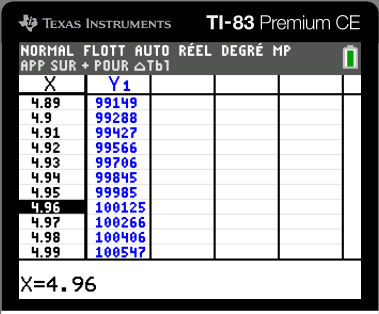
\includegraphics[scale=0.5]{01-12-06}
                        \end{center}
                    \end{enumMet}
                \end{enumMet}
            \end{bmethodet}



\graphicspath{{./1.11 - Application de la dérivation/img_cours/}}
\chapter{Application de la dérivation}
\thispagestyle{fancy}

%\vspace{-0.4cm}
\section{Étude des variations d'une fonction}

\begin{bthm}
	Soit une fonction $f$ définie et dérivable sur un intervalle I.
	\begin{itemProp}
		\item Si $f'(x)\leq 0$, alors $f$ est décroissante sur I.
		\item Si $f'(x)\geq 0$, alors $f$ est croissante sur I.
	\end{itemProp}
\end{bthm}

\subsection{Exemple d'une fonction du second degré}

\begin{bmethodet}{Étudier les variations d'une fonction polynôme du second degré}
\grasInMet{Enoncé :}
Soit la fonction f définie sur \R par $f(x)=2x^2-8x+1$.
\begin{enumMet}
	\item Calculer la fonction dérivée de $f$.
	\item Déterminer le signe de $f'$ en fonction de $x$.
	\item Dresser le tableau de variations de f.
\end{enumMet}
\ \\
%\newpage
\grasInMet{Réponse :}
\begin{enumMet}
\item Pour tout x réel, on a : $f'(x)=2\times 2x-8=4x-8$.
\item On commence par résoudre l'équation $f'(x)=0$.\\
Soit : $4x-8=0$\\
Donc $4x=8$  et $x= \dfrac{8}{4}=2$.\\
La fonction $f'$ est une fonction affine représentée par une droite dont le coefficient directeur 4 est positif.\\
Elle est donc d'abord négative (avant $x=2$) puis ensuite positive (après $x=2$).\\
%\newpage
\item On dresse alors le tableau de variations en appliquant le théorème :\\

\begin{center}
    \begin{tikzpicture}
        \tkzTabInit{$x$ / 0.8 , $f'(x)$ / 0.8, $f(x)$ / 1.4}{$-\infty$, $2$ ,$+\infty$}
        \tkzTabLine{, -,z , +,  }
        \tkzTabVar{+/  ,-/$-7$ ,  +/ }
    \end{tikzpicture}
	%\includegraphics[scale=1]{01-08-01.png}
\end{center}
\newpage
En effet : $f(2)=2\times 2^2-8\times 2+1=-7$.\\
La fonction f admet un minimum égal à $-7$ en $x=2$.\\
\end{enumMet}
\end{bmethodet}

\subsection{Exemple d'une fonction du troisième degré}

\begin{bmethodet}{Dresser le tableau de variations d'une fonction polynôme du 3e degré}
	Soit la fonction $f$ définie sur \R par $f(x)=x^3+\dfrac{9}{2} x^2-12x+5$.
	\begin{enumMet}
		\item Étudier les variations de $f$ et dresser le tableau de variation.
		\item Dans repère, représenter graphiquement la fonction f.
	\end{enumMet}
\ \\
\ \\
\begin{enumMet}
\item Pour tout $x$ réel, on a : $f'(x)=3x^2+9x-12$.\\
Commençons par résoudre l'équation $f'(x)=0$ :\\
Le discriminant du trinôme $3x^2+9x-12$ est égal à $\Delta = 92 - 4 \times 3 \times (–12) = 225$\\
L'équation possède deux solutions : $x_1= \dfrac{-9-\sqrt{225}}{2\times 3} = -4$ et $x_2= \dfrac{-9+\sqrt{225}}{2\times 3} = 1$\\
\\
On en déduit le tableau de variations de f :\\
\begin{center}
    \begin{tikzpicture}
        \tkzTabInit{$x$ / 0.8 , $f'(x)$ / 0.8, $f(x)$ / 2}{$-\infty$, $-4$,$1$ ,$+\infty$}
        \tkzTabLine{, +,z , -, z, +,  }
        \tkzTabVar{-/  ,+/$61$ ,  -/$-\dfrac{3}{2}$, +/ }
    \end{tikzpicture}
	%\includegraphics[scale=0.8]{01-08-02.png}
\end{center}
\item \ \\
\begin{center}
	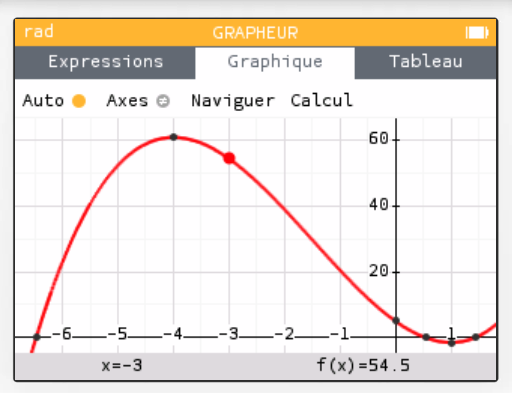
\includegraphics[scale=0.8]{Img_01}
\end{center}
\end{enumMet}
\end{bmethodet}

\section{Extremum d'une fonction}

\begin{bthm}
	Soit une fonction $f$ définie et dérivable sur un intervalle ouvert I.
    Si la dérivée $f'$ de $f$ s'annule et change de signe en un réel $c$ de I alors $f$ admet un extremum en $x = c$.
\end{bthm}

\begin{bmethodet}{Rechercher un extremum}
\grasInMet{Enoncé :}\\
	La fonction f définie sur \R par $f(x)=5x^2-3x+4$ admet-elle un extremum sur \R ?\\
	\ \\
\grasInMet{Réponse :}\\
Pour tout x réel, on a : $f'(x)=10x-3$ \\
Et : $f'(x)=0$ pour $x=\dfrac{3}{10}$.\\
\\
On dresse alors le tableau de variations :\\
\begin{center}
    \begin{tikzpicture}
        \tkzTabInit{$x$ / 1 , $f'(x)$ / 0.8, $f(x)$ / 2}{$-\infty$, $\dfrac{3}{10}$ ,$+\infty$}
        \tkzTabLine{, -,z , +,  }
        \tkzTabVar{+/  ,-/$\dfrac{71}{20}$ ,  +/ }
    \end{tikzpicture}
	%\includegraphics[scale=1]{01-08-04.png}
\end{center}
En effet : $f\left(\dfrac{3}{10}\right)=\dfrac{71}{20}$\\
La fonction $f$ admet donc un minimum égal à $\dfrac{71}{20}$ en $x= \dfrac{3}{10}$.\\
\end{bmethodet}

\section{Position relative de deux courbes}
\begin{bmethodet}{Position relative de deux courbes}
    \grasInMet{Enoncé :}\\
    Soit $f$ et $g$ deux fonctions définies sur $[2 ; +\infty [$ par : $f(x)=x^3$ et $g(x)=-5x+18$.\\
    Étudier la position relative des courbes représentatives $C_f$ et $C_g$.\\
    \ \\
    \grasInMet{Réponse :}\\
    On va étudier le signe de la différence $f(x)-g(x)$ :\\
    On pose : $h(x)=f(x)-g(x)=x^3+5x-18$.\\
     \\
    Pour tout $x$ de $[2 ; +\infty [$, on a : \\
    $h'(x)=3x^2+5$\\
    Donc  $h'(x)>0$.
    On en déduit que la fonction f est strictement croissante sur $[2 ; +\infty [$.
    
    On construit le tableau de variations :\\
    \begin{center}
    \begin{tikzpicture}
        \tkzTabInit{$x$ / 0.8 , $h'(x)$ / 0.8, $h(x)$ / 1.6}{$2$ ,$+\infty$}
        \tkzTabLine{, +,  }
        \tkzTabVar{-/$0$ ,  +/ }
    \end{tikzpicture}
	%\includegraphics[scale=0.8]{01-08-05.png}
    \end{center}
    
    $h(2)=2^3+5\times 2-18=0$\\
    D'après le tableau de variations, on a $h(x)\geq 0$.\\
    Soit : $f(x)-g(x)\geq 0$ et donc  $f(x)\geq g(x)$.\\ 
    On en déduit que la courbe $C_f$ est au-dessus de la courbe $C_g$ sur l'intervalle $[2 ; +\infty [$.
\end{bmethodet}
\graphicspath{{images/}}
\chapter{Variables aléatoires}
\thispagestyle{fancy}

\section{Variable aléatoire et loi de probabilité}

\subsection{Variable aléatoire}

\begin{bexemple}
Soit l'expérience aléatoire : \guillemets{On lance un dé à six faces et on regarde le résultat.} \\
L'ensemble de toutes les issues possibles $E = \{1 ; 2 ; 3 ; 4 ; 5 ; 6\}$ s'appelle l'univers des possibles. Il se note $\Omega$.\\
On considère le jeu suivant :\\
\begin{itemEx}
\item Si le résultat est pair, on gagne \EUR{2}.
\item Si le résultat est 1, on gagne \EUR{3}.
\item Si le résultat est 3 ou 5, on perd \EUR{4}.
\end{itemEx}
On peut définir ainsi une variable aléatoire $X$ sur $E = \{1 ; 2 ; 3 ; 4 ; 5 ; 6\}$ qui peut prendre les valeurs $2$, $3$ ou $-4$.

Pour les issues $2$, $4$ ou $6$, on a : $X = 2$
Pour l'issue $1$, on a : $X = 3$
Pour les issues $3$ et $5$, on a : $X = -4$.
\end{bexemple}

\begin{bdefi}
Une \grasInDef{variable aléatoire X} associe un nombre réel à chaque issue de l'univers $\Omega$.\\
\end{bdefi}

\subsection{Loi de probabilité}

\begin{bdefi}
    La \grasInDef{probabilité de l’événement} $\{X=x_i\}$ est la somme des probabilités des issues de $X$ auxquelles on associe le réel $x_i$.
\end{bdefi}

\begin{bdefi}
    Soit $X$ une variable aléatoire définie sur $\Omega$. \grasInDef{Définir la loi de probabilité} de la variable aléatoire $X$, c’est associer à chaque valeur $x_i$ prise par $X$ la probabilité de l’événement $\{X=x_i\}$.\\
    On présente souvent la loi de probabilité de X sous la forme d’un tableau.\\
    
    \begin{tabular}{ | Xc | Xc | Xc | Xc | Xc |}
     \hline			
       $x_i$  & $x_1$ & $x_2$ & ... & $x_n$ \\ \hline
       $P(X=x_i)$ & $p_1$ & $p_2$ & ... & $p_n$ \\
     \hline  
    \end{tabular}
    
\end{bdefi}

\begin{bexemple}
    On considère la variable aléatoire $X$ définie dans l'exemple précédent.\\
    Chaque issue du lancer de dé est équiprobable et égale à $\dfrac{1}{6}$.
    La probabilité que la variable aléatoire prenne la valeur $2$ est égale à $\dfrac{1}{6} + \dfrac{1}{6} + \dfrac{1}{6} = \dfrac{1}{2}$.\\
    On note : $P(X = 2) = \dfrac{1}{2}$.\\
    De même : $P(X = 3) = \dfrac{1}{6}$ et $P(X = -4) = \dfrac{1}{6} + \dfrac{1}{6} = \dfrac{1}{3}$.
    \\
    On peut résumer les résultats dans un tableau :\\
    \ \\
    \begin{tabular}{ | Xc | Xc | Xc | Xc | }
     \hline			
       $x_i$  & $-4$ & $2$ & $3$ \\ \hline
       $P(X=x_i)$ & $\dfrac{1}{3}$ & $\dfrac{1}{2}$ & $\dfrac{1}{6}$ \\
     \hline  
    \end{tabular}\\
    \ \\
    Ce tableau résume la loi de probabilité de la variable aléatoire X.
\end{bexemple}


\begin{brmqs}
    \begin{itemRem}
        \item $P(X = x_i)$ peut se noter $p_i$.
        \item $p_1 + p_2 + ... + p_n = 1$
    \end{itemRem}
\end{brmqs}

\begin{bexemple}
    Dans l'exemple traité plus haut : $p_1 + p_2 + p_3 = \dfrac{1}{3} + \dfrac{1}{2} + \dfrac{1}{6} = 1$.
\end{bexemple}

\begin{bmethodet}{Déterminer une loi de probabilité}
    Soit l'expérience aléatoire : \guillemets{On tire une carte dans un jeu de $32$ cartes.}\\
    On considère le jeu suivant :
    \begin{itemMet}
        \item Si on tire un cœur, on gagne \EUR{2}.
        \item Si on tire un roi, on gagne \EUR{5}.
        \item Si on tire une autre carte, on perd \EUR{1}.
    \end{itemMet}
    On appelle $X$ la variable aléatoire qui, à une carte tirée, associe un gain ou une perte.\\
    1) Déterminer la loi de probabilité de $X$.\\
    2) Calculer $P(X \geq 5)$ et interpréter le résultat.\\
    \\
    \\
    1) La variable aléatoire $X$ peut prendre les valeurs $2$, $5$, $-1$ mais aussi $7$.\\
    En effet, si on tire le roi de cœur, on gagne $5$(roi) + $2$(cœur) = \EUR{7}.\\
    \begin{itemMet}
        \item Si la carte tirée est un cœur (autre que le roi de cœur), $X = 2$.\\
        $P(X = 2) = \dfrac{7}{32}$.
        \item Si la carte tirée est un roi (autre que le roi de cœur), $X = 5$.\\
        $P(X = 5) = \dfrac{3}{32}$.
        \item Si la carte tirée est le roi de cœur, $X = 7$.\\
        $P(X = 7) = \dfrac{1}{32}$.
        \item Si la carte tirée n'est ni un cœur, ni un roi, $X = -1$.\\
        $P(X = -1) = \dfrac{21}{32}$.
    \end{itemMet}
    La loi de probabilité de X est :\\
    \begin{tabular}{ | Xc | Xc | Xc | Xc | Xc |}
         \hline			
           $x_i$  & $-1$ & $2$ & $5$ & $7$ \\ \hline
           $p_i$ & $\dfrac{21}{32}$ & $\dfrac{7}{32}$ & $\dfrac{3}{32}$ & $\dfrac{1}{32}$ \\
         \hline  
    \end{tabular}
    \ \\
    \ \\
    On constate que : $p_1 + p_2 + p_3 + p_4  = \dfrac{21}{32} + \dfrac{7}{32} + \dfrac{3}{32} + \dfrac{1}{32} = 1$\\
    \ \\
    2) $P(X \geq 5) = P(X = 5) + P(X = 7) = \dfrac{3}{32} + \dfrac{1}{32} = \dfrac{4}{32} = \dfrac{1}{8}$\\
    La probabilité de gagner plus de \EUR{5} est égale à $\dfrac{1}{8}$.
\end{bmethodet}

\section{Espérance, variance et écart-type}

\subsection{Espérance}

\begin{bdefi}
L'espérance mathématique de la loi de probabilité de $X$ est le nombre réel, noté $E(X)$, défini par :\\
        $$E(X) = \sum_{i=1}^{n} p_ix_i = p_1x_1 + p_2x_2 + ... + p_nx_n$$
\end{bdefi}

\begin{bmethodet}{Déterminer une loi de probabilité}
    Dans le jeu de la \guillemets{Méthode} du paragraphe précédent, calculer l'espérance de la loi de probabilité de X et interpréter le résultat.\\
    \ \\
    	$E(X) = \dfrac{21}{32} \times (-1)+ \dfrac{7}{32} \times 2+ \dfrac{3}{32} \times 5+\dfrac{1}{32} \times 7=\dfrac{15}{32}$\\
    L'espérance est égale à $\dfrac{15}{32}\approx 0,5$ signifie qu'en jouant un grand nombre de fois, on peut espérer gagner environ \EUR{0,50} par partie.
\end{bmethodet}

\begin{brmq}
    L'espérance est donc le gain moyen par partie que l'on peut espérer si l'on répète l'expérience un grand nombre de fois. Dans tous les jeux au casino l'espérance est négative. Sur un grand nombre de parties, c'est le casino qui est gagnant.
\end{brmq}

\subsection{Variance et écart-type}

\begin{bdefis}

    \begin{itemDef}
        \item La variance de $X$ est le nombre réel, noté $Var(X)$, défini par :\\
        $$Var(x) = \sum_{i=1}^{n} p_i(x_i-E(X))^2 = p_1(x_1-E(X))^2 + p_2(x_2-E(X))^2 + ... + p_n(x_n-E(X))^2$$
        \item L'écart-type de $X$ est le nombre réel, noté $\sigma(X)$, défini par, $\sigma(X)=\sqrt{Var(X)}$\\
    \end{itemDef}
\end{bdefis}

\begin{bmethodet}{Déterminer une variance et un écart-type}
    Dans le jeu de la \guillemets{Méthode} précédente, calculer la variance et l'écart-type.\\
    On rappelle que $E(X) =\dfrac{15}{32}$\\
    $Var(X) = \dfrac{21}{32} \times (-1-\dfrac{15}{32})^2+ \dfrac{7}{32} \times (2-\dfrac{15}{32})^2+ \dfrac{3}{32} \times (5-\dfrac{15}{32})^2+\dfrac{1}{32} \times (7-\dfrac{15}{32})^2=\dfrac{5311}{1024}\approx 5,19$\\
	$\sigma(X)=\sqrt{Var(X)}=\sqrt{\dfrac{5311}{1024}}\approx 2,28$\\
    L'écart-type est d'environ $2,28$. Plus l'écart-type est petit, plus les résultats des parties seront proches de l'espérance. Un grand écart-type signifie donc que vous pouvez avoir des résultats très différents que ce qui est prévu (en positif comme en négatif).
\end{bmethodet}
\chapter{Variations de suites}
\thispagestyle{fancy}


\section{Sens de variation d'une suite numérique}

\begin{bexemple}
On a représenté ci-dessous le nuage de points des premiers termes d'une suite $\left(u_{n}\right)$ :
\begin{center}
    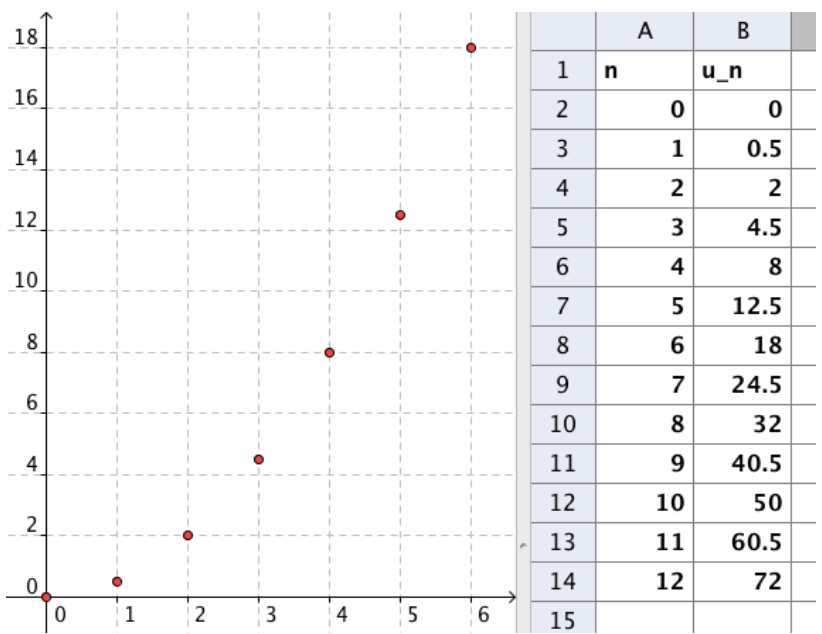
\includegraphics[scale=0.4]{1.08.00-Img04}
\end{center}
On peut conjecturer que cette suite est croissante. On constate par exemple que $u_{1}<u_{2}$ ou encore $u_{4}<u_{5}$. De manière générale, on peut écrire : $u_{n}<u_{n+1}$
\end{bexemple}

\begin{bdefis}
Soit une suite numérique $\left(u_{n}\right)$.
\begin{itemDef}
\item La \grasInDef{suite $\left(u_{n}\right)$ est croissante} signifie que pour tout entier $n$, on a $u_{n+1} \geqslant u_{n}$.
\item La \grasInDef{suite $\left(u_{n}\right)$ est décroissante} signifie que pour tout entier $n$, on a $u_{n+1} \leqslant u_{n}$.
\end{itemDef}
\end{bdefis}

\begin{bmethodet}{Étudier les variations d'une suite}
\grasInMet{Énoncé:}
\begin{enumMet}
\item Pour tout $n$ de $\mathbb{N}$, on donne la suite $\left(u_{n}\right)$ définie par : $u_{n+1}=u_{n}+2$.\\
Démontrer que la suite $\left(u_{n}\right)$ est croissante.
\item Pour tout $n$ de $\mathbb{N}$, on donne la suite $\left(v_{n}\right)$ définie par : $v_{n}=4 n+4$.\\
Démontrer que la suite $\left(v_{n}\right)$ est croissante.
\end{enumMet}
\grasInMet{Réponse:}
\begin{enumMet}
\item $u_{n+1}-u_{n}=2>0$\\
On en déduit que $\left(u_{n}\right)$ est croissante.
\item On commence par calculer la différence $v_{n+1}-v_{n}$ :\\
On a $: v_{n}=4 n+4$ donc $v_{\mVert{n+1}}=4\mVert{(n+1)}+4=4 n+4+4=4 n+8$
\begin{align*}
v_{n+1}-v_{n}&=4 n+8-(4 n+4) \\
&=4 n+8-4 n-4 \\
&=4
\end{align*}
On étudie ensuite le signe de $v_{n+1}-v_{n}$ :\\
Pour tout $n$ entier $v_{n+1}-v_{n}=4>0$.\\
On en déduit que la suite $\left(v_{n}\right)$ est croissante.
\end{enumMet}
\end{bmethodet}


\section{variation d'une suite arithmétique}

\begin{bprop}
    $U_n$ est une suite arithmétique de raison $r$.
    \begin{itemDef}
    	\item Si $r > 0$ alors la suite $U_n$ est croissante.
    	\item Si $r < 0$ alors la suite $U_n$ est décroissante.
    \end{itemDef}
\end{bprop}

\begin{bdemo}
    $U_{n+1}-U_n=U_n+r-U_n=r$.
    \begin{itemDem}
    	\item Si $r > 0$ alors $U_{n+1}-U_n>0$  et la suite $U_n$ est croissante.
    	\item Si $r < 0$ alors $U_{n+1}-U_n<0$ et la suite $U_n$ est décroissante.
    \end{itemDem}
\end{bdemo}
\begin{bexemple}
    La suite arithmétique $U_n$ définie par $U_n=8-3n$ est décroissante car de raison négative et égale à $-3$.
\end{bexemple}


\section{variation d'une suite géométrique}

\begin{bprop}
    $U_n$ est une suite géométrique de raison $q$ et de premier terme non nul $U_0$.\\
    Pour $U_0>0$ :
    \begin{itemProp}
    	\item Si $q > 1$ alors la suite $U_n$ est croissante.
    	\item Si $0 < q < 1$ alors la suite $U_n$ est décroissante.
    \end{itemProp}
    Pour $U_0<0$ :
    \begin{itemDef}
    	\item Si $q > 1$ alors la suite $U_n$ est décroissante.
    	\item Si $0 < q < 1$ alors la suite $U_n$ est croissante.
    \end{itemDef}
\end{bprop}

\begin{bdemot}{cas où $U_0 > 0$ }
    $U_{n+1}-U_n=U_0\times q^{n+1}-U_0\times q^n=U_0\times q^n\times (q-1)$.
    \begin{itemDem}
    	\item Si $q > 1$ alors $U_{n+1}-U_n>0$ et la suite $U_n$ est croissante.
    	\item Si $0 < q < 1$ alors $U_{n+1}-U_n<0$ et la suite $U_n$ est décroissante.
    \end{itemDem}
\end{bdemot}





\chapter{Application du produit scalaire}
\thispagestyle{fancy}

    \section{Produit scalaire et norme}
    
    \subsection{Propriétés}

    % Soit un vecteur $\vv{u},$ on a :
    % $\vv{u} \cdot \vv{u}=\|\vv{u}\| \times\|\vv{u}\| \times \cos (\vv{u} ; \vv{u})=\|\vv{u}\|^{2} \times \cos 0=\|\vv{u}\|^{2}$\\
    % et\\
    % $\vv{u}\cdot \vv{u}=\vv{u}^{2}$\\
    % On a ainsi $: \vv{u}^{2}=\vv{u} \cdot \vv{u}=\|\vv{u}\|^{2}$
    
    \begin{bprop}
        Propriété : Soit $\vv{u}$ et $\vv{v}$ deux vecteurs. On a :
        \begin{itemDef}
            \item $\vv{u} \cdot \vv{v}=\dfrac{1}{2}\left(\|\vv{u}\|^{2}+\|\vv{v}\|^{2}-\|\vv{u}-\vv{v}\|^{2}\right)$
            \item $\vv{u} \cdot \vv{v}=\dfrac{1}{2}\left(\|\vv{u}+\vv{v}\|^{2}-\|\vv{u}\|^{2}-\|\vv{v}\|^{2}\right)$
            \item $\vv{u} \cdot \vv{v}=\dfrac{1}{4}\left(\|\vv{u}+\vv{v}\|^{2}-\|\vv{u}-\vv{v}\|^{2}\right)$
        \end{itemDef}
    \end{bprop}
    
    \begin{bdemot}{Démonstration de la première formule}
        \begin{align*}
            \|\vv{u}-\vv{v}\|^{2}&=(\vv{u}-\vv{v})^{2} \\
            &=\vv{u}^{2}-2 \vv{u} \cdot \vv{v}+\vv{v}^{2} \\
            &=\|\vv{u}\|^{2}-2 \vv{u} \cdot \vv{v}+\|\vv{v}\|^{2}
        \end{align*}
        Donc $\vv{u} \cdot \vv{v}=\dfrac{1}{2}\left(\|\vv{u}\|^{2}+\|\vv{u}\|^{2}-\|\vv{u}-\vv{v}\|^{2}\right)$
    \end{bdemot}

    \begin{bprop}
        Soit $A, B$ et $C$ trois points du plan. On a :
        $\vv{A B} \cdot \vv{A C}=\dfrac{1}{2}\left(A B^{2}+A C^{2}-B C^{2}\right)$
    \end{bprop}
    
    \begin{bdemo}
        \begin{align*}
            \vv{A B} \cdot \vv{A C}&=\dfrac{1}{2}\left(\|\vv{A B}\|^{2}+\|\vv{A C}\|^{2}-\|\vv{A B}-\vv{A C}\|^{2}\right) \\
            &=\dfrac{1}{2}\left(A B^{2}+A C^{2}-\|\vv{C B}\|^{2}\right) \\
            &=\dfrac{1}{2}\left(A B^{2}+A C^{2}-B C^{2}\right)
        \end{align*}
    \end{bdemo}
    
    \begin{bexemple}
        Si $\mathrm{AB}=6, \mathrm{AC}=5$ et $\mathrm{CB}=4$ alors:
        $$
        \vv{A B} \cdot \vv{A C}=\frac{1}{2}\left(A B^{2}+A C^{2}-C B^{2}\right)=\frac{1}{2}\left(6^{2}+5^{2}-4^{2}\right)=\frac{1}{2}(36+25-16)=\frac{45}{2}
        $$
    \end{bexemple}
    
    \begin{bmethodet}{Calculer un produit scalaire à l'aide des normes}
        \grasInMet{Enoncé :}\\
        On considère la figure ci-dessous, calculer le produit scalaire $\vv{C G} \cdot \vv{C F}$
        \begin{center}
            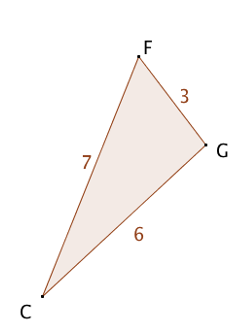
\includegraphics[scale=0.8]{1.04.IMG-02}
        \end{center}
        \ \\
        \grasInMet{Réponse :}\\
        $\vv{C G} \cdot \vv{C F}=\frac{1}{2}\left(C G^{2}+C F^{2}-G F^{2}\right)$\\
        $=\dfrac{1}{2}\left(6^{2}+7^{2}-3^{2}\right)$\\
        $=38$
    \end{bmethodet}
    
    \subsection{Théorème d'Al Kashi}
    
    \begin{bthm}
        Dans un triangle $\mathrm{ABC},$ on a, avec les notations de la figure :
        $$
        a^{2}=b^{2}+c^{2}-2 b c \cos \hat{A}
        $$
        \begin{center}
            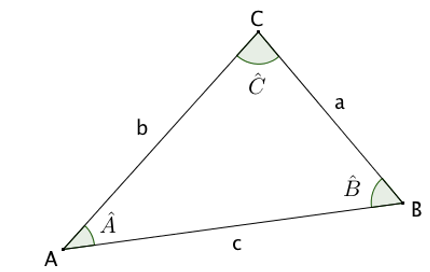
\includegraphics[scale=0.8]{1.04.IMG-03}
        \end{center}
    \end{bthm}
    
    \begin{bdemo}
        $\vv{A B} \cdot \vv{A C}=A B \times A C \times \cos \hat{A}=b c \cos \hat{A}$\\
        et\\
        $\vv{A B} \cdot \vv{A C}=\frac{1}{2}\left(A B^{2}+A C^{2}-B C^{2}\right)=\frac{1}{2}\left(b^{2}+c^{2}-a^{2}\right)$\\
        Donc $: \frac{1}{2}\left(b^{2}+c^{2}-a^{2}\right)=b c \cos \hat{A}$\\
        Soit $: b^{2}+c^{2}-a^{2}=2 b c \cos \hat{A}$\\
        Soit encore $: a^{2}=b^{2}+c^{2}-2 b c \cos \hat{A}$\\
    \end{bdemo}
    
    \begin{bmethodet}{Calculer un angle à l'aide des normes}
        \grasInMet{Enoncé :}\\
        On considère la figure ci-dessous, calculer la mesure de l'angle $\widehat{B A C}$ au degré près.
        \begin{center}
            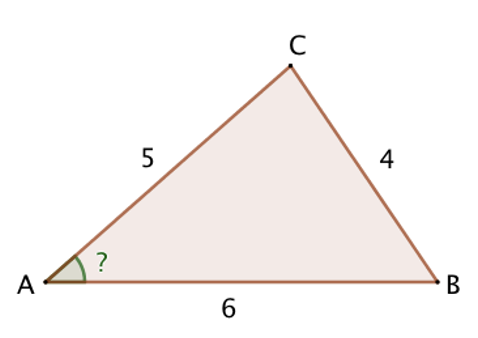
\includegraphics[scale=0.8]{1.04.IMG-05}
        \end{center}
        \ \\
        \grasInMet{Réponse :}\\
        D'après le théorème d'Al Kashi, on a :\\
        $C B^{2}=A B^{2}+A C^{2}-2 \times A B \times A C \times \cos \widehat{B A C}$\\
        $4^{2}=6^{2}+5^{2}-2 \times 6 \times 5 \times \cos \widehat{B A C}$\\
        $16=36+25-60 \cos \widehat{B A C}$\\
        $60 \cos \widehat{B A C}=36+25-16$\\
        $60 \cos \widehat{B A C}=45$\\
        $\cos \widehat{B A C}=\dfrac{45}{60}$\\
        $\cos \widehat{B A C}=\dfrac{3}{4}$\\
        $\widehat{B A C} \approx 41^{\circ}$
    \end{bmethodet}
    
    \section{Vecteur Normal}
    
    \subsection{définition et propriétés}
    
    \begin{bdefi}
        Un \grasInDef{vecteur normal} à une droite $d$ quelconque du plan est un vecteur non nul et orthogonal à un vecteur directeur de $d$.
    \end{bdefi}
    
    \begin{bprop}
        Deux droites du plan sont perpendiculaires si et seulement si un vecteur normal de l'une est orthogonal à un vecteur normal de l'autre.
    \end{bprop}
    
    \begin{bdemo}
        On suppose que $d$ et $d^{\prime}$ sont perpendiculaires. Si $\vv{u}$ est un vecteur directeur de $d$ et $\vv{v}$ de $d^{\prime},$ alors $\vv{u}$ et $\vv{v}$ sont orthogonaux. $\vv{v}$ étant normal à $d$ et $\vv{u}$ à $d^{\prime},$ la propriété est vérifiée.\\
        Réciproquement, si $\vv{u},$ vecteur normal à $d,$ est orthogonal à $\vv{v},$ vecteur normal à $d^{\prime},$ alors $\vv{v}$ est un vecteur directeur de $d$ et $\vv{u}$ de $d^{\prime} .$ Ayant des vecteurs directeurs orthogonaux, d et $d^{\prime}$ sont perpendiculaires.
    \end{bdemo}
    
    \begin{bmethode}
        \grasInMet{Enoncé:}\\
        Soit $d$ une droite de vecteur directeur $\Coord{u}{3}{5}$.
        \begin{enumMet}
            \item Déterminer une condition sur les coordonnées d'un vecteur $\vv{n}$ non nul pour qu'il soit normal à $d$.
            \item Le vecteur $\Coord{v}{-10}{6}$ est-il un vecteur normal à $d$?
        \end{enumMet}
        
        \grasInMet{Réponse:}\\
        \begin{enumMet}
            \item Si $\Coord{n}{x}{y}$ est un vecteur normal à $d$, alors il est orthogonal à $\vv{u}$.\\
            Donc $\vv{u} \cdot \vv{n}=3 x+5 y=0$ soit $y=-\dfrac{3}{5} x$.\\
            Les coordonnées de $\vv{n}$ sont donc de la forme $\CoordSV{x}{-\dfrac{3}{5}x}$ avec $x \in \R$.
            \item On calcule le produit scalaire $\vv{u}\cdot\vv{v}$\\
            $\vv{u}\cdot\vv{v}=3\times(-10)+5\times6=-30+30=0$\\
            le vecteur $\vv{v}$ est orthogonal au vecteur directeur $\vv{u}$ de la droite $d$, donc $\vv{v}$ est un vecteur normal à $d$. 
        \end{enumMet}
    \end{bmethode}
    
    \subsection{Équations cartésiennes et vecteur normal}
    
    \begin{brappel}
        Toute droite $D$ admet une équation de la forme $a x+b y+c=0$ avec $(a ; b) \neq(0 ; 0) .$ Un \grasInDef{vecteur directeur} de $D$ est $\Coord{u}{-b}{a}$ \\
        Cette équation est appelée \grasInDef{équation cartésienne} de la droite $D$.
    \end{brappel}
        
    \begin{bprop}
        Soient $a, b$ et $c$ trois réels tels que $a$ et $b$ ne sont pas simultanément nuls.\\
        La droite d'équation cartésienne $a x+b y+c=0$ admet pour \grasInDef{vecteur normal} le vecteur $\Coord{n}{a}{b}$.\\
        \ \\
        Réciproquement, toute droite ayant pour \grasInDef{vecteur normal} le vecteur non nul $\Coord{n}{a}{b}$ admet une équation cartésienne de la forme $a x+b y+c=0$.
    \end{bprop}
        
    \begin{bexemple}
        La droite d'équation cartésienne $3 x-4 y+5=0$ admet pour vecteur normal le vecteur $\Coord{n}{3}{-4}$  et pour vecteur directeur le vecteur $\Coord{u}{4}{3}$.\\
        On a bien $\vv{n} \cdot \vv{u}=0$
    \end{bexemple}
    
    \begin{bmethode}
        \grasInMet{Enoncé:}\\
        Dans un repère orthonormé, déterminer, de deux façons différentes, une équation cartésienne de la droite $d$ passant par le point $\mathrm{A}(5 ;-1)$ et de vecteur normal $\Coord{n}{2}{-3}$.
        
        \grasInMet{Réponse:}\\
        \begin{enumMet}
            \item 1. On lit sur le vecteur normal que $a=2$ et $b=-3$.
            Donc une équation de $d$ est de la forme $2 x-3 y+c=0$. $\mathrm{A}(5 ;-1) \in d$ donc $2 \times 5-3 \times(-1)+c=0$ et donc $c=-13$.\\
            Ainsi, une équation de la droite $d$ est $2 x-3 y-13=0$.
            \item Soit $\mathrm{M}(x ;y)$ appartenant à $d .$ Alors $\vv{\mathrm{AM}}$ est un vecteur directeur de $d$ et est orthogonal au vecteur $\vv{n}$.\\
            $\vv{\mathrm{AM}} \cdot \vv{n}=0 \iff \CoordSV{x-5}{y+1} \cdot \CoordSV{2}{-3}=0 \iff 2(x-5)-3(y+1)=0 \iff 2 x-3 y-13=0$\\
            Donc une équation de la droite $d$ est $2 x-3 y-13=0$
        \end{enumMet}
    \end{bmethode}




\end{document}